After-pulsing and cross-talk comparison for KETEK PM1125NS-SB0, Hamamatsu S10362-11-100C and Hamamatsu S13360-3050CS.

\section{Abstract}
Silicon photomultipliers (SiPM) have become widespread recently.
They exceed photomultipliers on quantum efficiency, size and resistance to the magnetic field.
However, due to the features of the structure they have a greater value of dark noise, as well as have additional sources of noise: cross-talk and after-pulsing.
In addition, these parameters may have a temperature dependence.

In this article one study dark noise, probabilities of cross-talk and after-pulsing at different voltages and temperatures for two modern SiPM: Hamamatsu S13360-3050CS and KETEK PM1125NS-SB0 and Hamamatsu S10362-11-100C SiPM from previous generation.
An offline signal processing was performed by a pulse approximation with reconstruction of amplitudes
and start times to find these parameters.
As a result, we found that in achieved measurement accuracy dark noise has a temperature and voltage dependence, but cross-talk and after-pulsing probabilities have only the latter.

The measured cross-talk probabilities for KETEK PM1125NS-SB0 and Hamamatsu S13360-3050CS at their operating voltage is about 6\%
which is two times smaller than that for Hamamatsu S10362-11-100C.
The total after-pulsing probability (fast component) for KETEK PM1125NS-SB0 and Hamamatsu S13360-3050CS is about 12\%, which is also almost 2 times smaller than that for Hamamatsu S10362-11-100C (fast and slow component).
Dark noise rate for Hamamatsu S13360-3050CS at $ 20 \; ^{\circ}C $ is only $ 30 \; kHz / mm ^ 2 $ in comparison with $ 80 \; kHz / mm ^ 2 $ for KETEK PM1125NS-SB0.

\section{Introduction}
BINP many years engaged in the development of X-ray inspection systems \cite{SiPM based photon counting detector for scanning digital radiography}.
These installations can be used in various fields: inspection at airports, subways or at workplaces.
Multistrip ionization chamber filled with pure Xe at 15 bar have been used as X-ray detector until now.
However, this detector has a serious disadvantage - it works in the integrating mode, so at low input flow of particles electronic noise seriously degrades quality of images.
Another disadvantage is the insufficiently high detection efficiency of high-energy photons.
In this regard, it was decided to choose a new detector based on SiPM and a scintillator which may have a detection efficiency > 90 \% and operate in the mode of direct photon counting.

The main purpose of this work is to measure after-pulsing and cross-talk probabilities for two SiPM: KETEK PM1125NS-SB0 and Hamamatsu S13360-3050CS and compare them with characteristics of Hamamatsu S10362-11-100C - the device from previous generation.
\section{Measurement of breakdown voltage}
One of important characteristics of any SiPM is a breakdown voltage.
A breakdown voltage $ V_ {BD} $ is a voltage at which a gain equals to zero.

In many works are shown that various SiPMs gain is a linear function of both a temperature and a voltage.
Thus, the expression for a gain $ G (V, T) $ is written as follows: \cite{Silicon Photomultiplier's Gain Stabilization, Temperature and Bias Voltage Dependence, Characterization of SiPM: temperature dependencies, Characterisation of a silicon photomultiplier device}:
\begin{eqnarray}\label{eq:G(V, T)}
G(V, T) = a \cdot V + b \cdot T + c
\end{eqnarray}

It is easy to find a breakdown voltage equating the gain from Eq.(\ref{eq:G(V, T)}) to zero :
\begin{eqnarray}\label{eq:V_bd(T)}
V_{BD}(T) = \frac{-(b \cdot T + c)}{a} = \frac{dV}{dT} \cdot T + const
\end{eqnarray}

The following installation was assembled for measurement of a breakdown voltage and a gain (Fig.~\ref{image:install_V_bd}).
The light source based on fast LED (CAEN SP5601) sends a flash through an optical fiber to SiPM.
At the same time, the light source sends a trigger signal to the CAEN DT5720A ADC.
The signal from the SiPM passes through the amplifier to the CAEN DT5720A, which integrates the signal in the presence of the trigger signal.
The resulting charge is transmitted to computer in on-line mode.
SiPM is mounted on a thermoelectric cooler and the temperature stabilization is ensured by TRM 101 PID - controller.
The deviation from the set temperature does not exceed 1K.
\begin{figure}[h]
\center{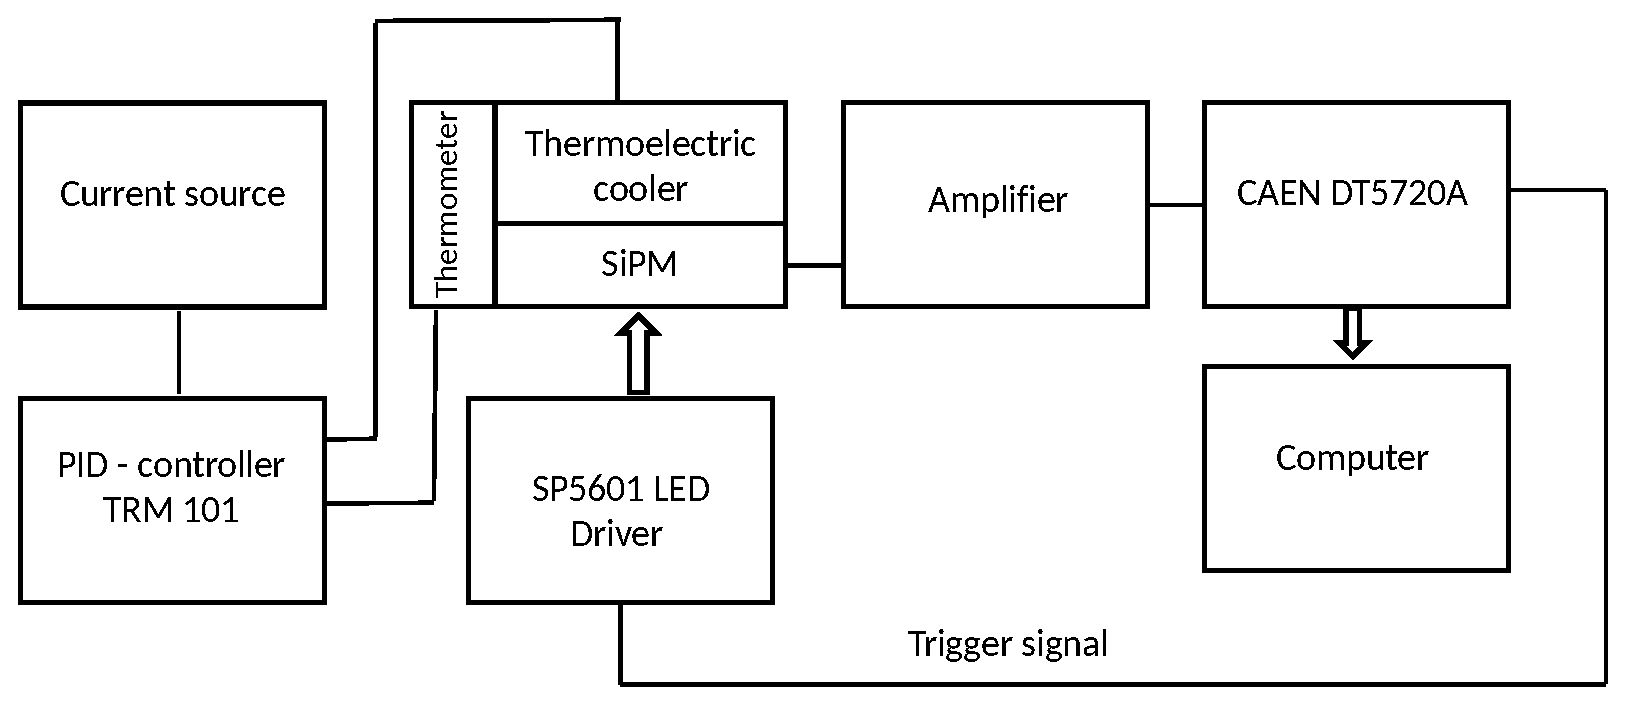
\includegraphics[width=8cm]{install_V_bd_11}}
\caption{The Installation scheme for measurement the SiPM breakdown voltage.}
\label{image:install_V_bd}
\end{figure}

The calculation of the breakdown voltage had several stages.
The intensity of the light source was set so that there were not SiPM triggering or single photon was registered in generally.
The signal was integrated into the gate with 200 ns duration ($\approx 5 \cdot \tau$).
Then the tops of the noise peak and the peak from the registration of single photons waere approximated by a Gaussian function.
We calculated the distance $\Delta$ between the 0th and the 1st peak.
Distances between the first and the second, the second and the third etc. peaks were not considered.
The main reason was that as the number of peak increased the greater became the discrepancy between the true and measured peak position because of after-pulses.
An example of charge spectrum is shown in Fig.~\ref{image:sipm_spectrum}.
In measurements an voltage error $\Delta V$ was estimated at 0.01 V, and a temperature error $\Delta T$ was estimated as the minimum temperature step 1 K divided by $\sqrt{12}$.

\begin{figure}[h]
\center{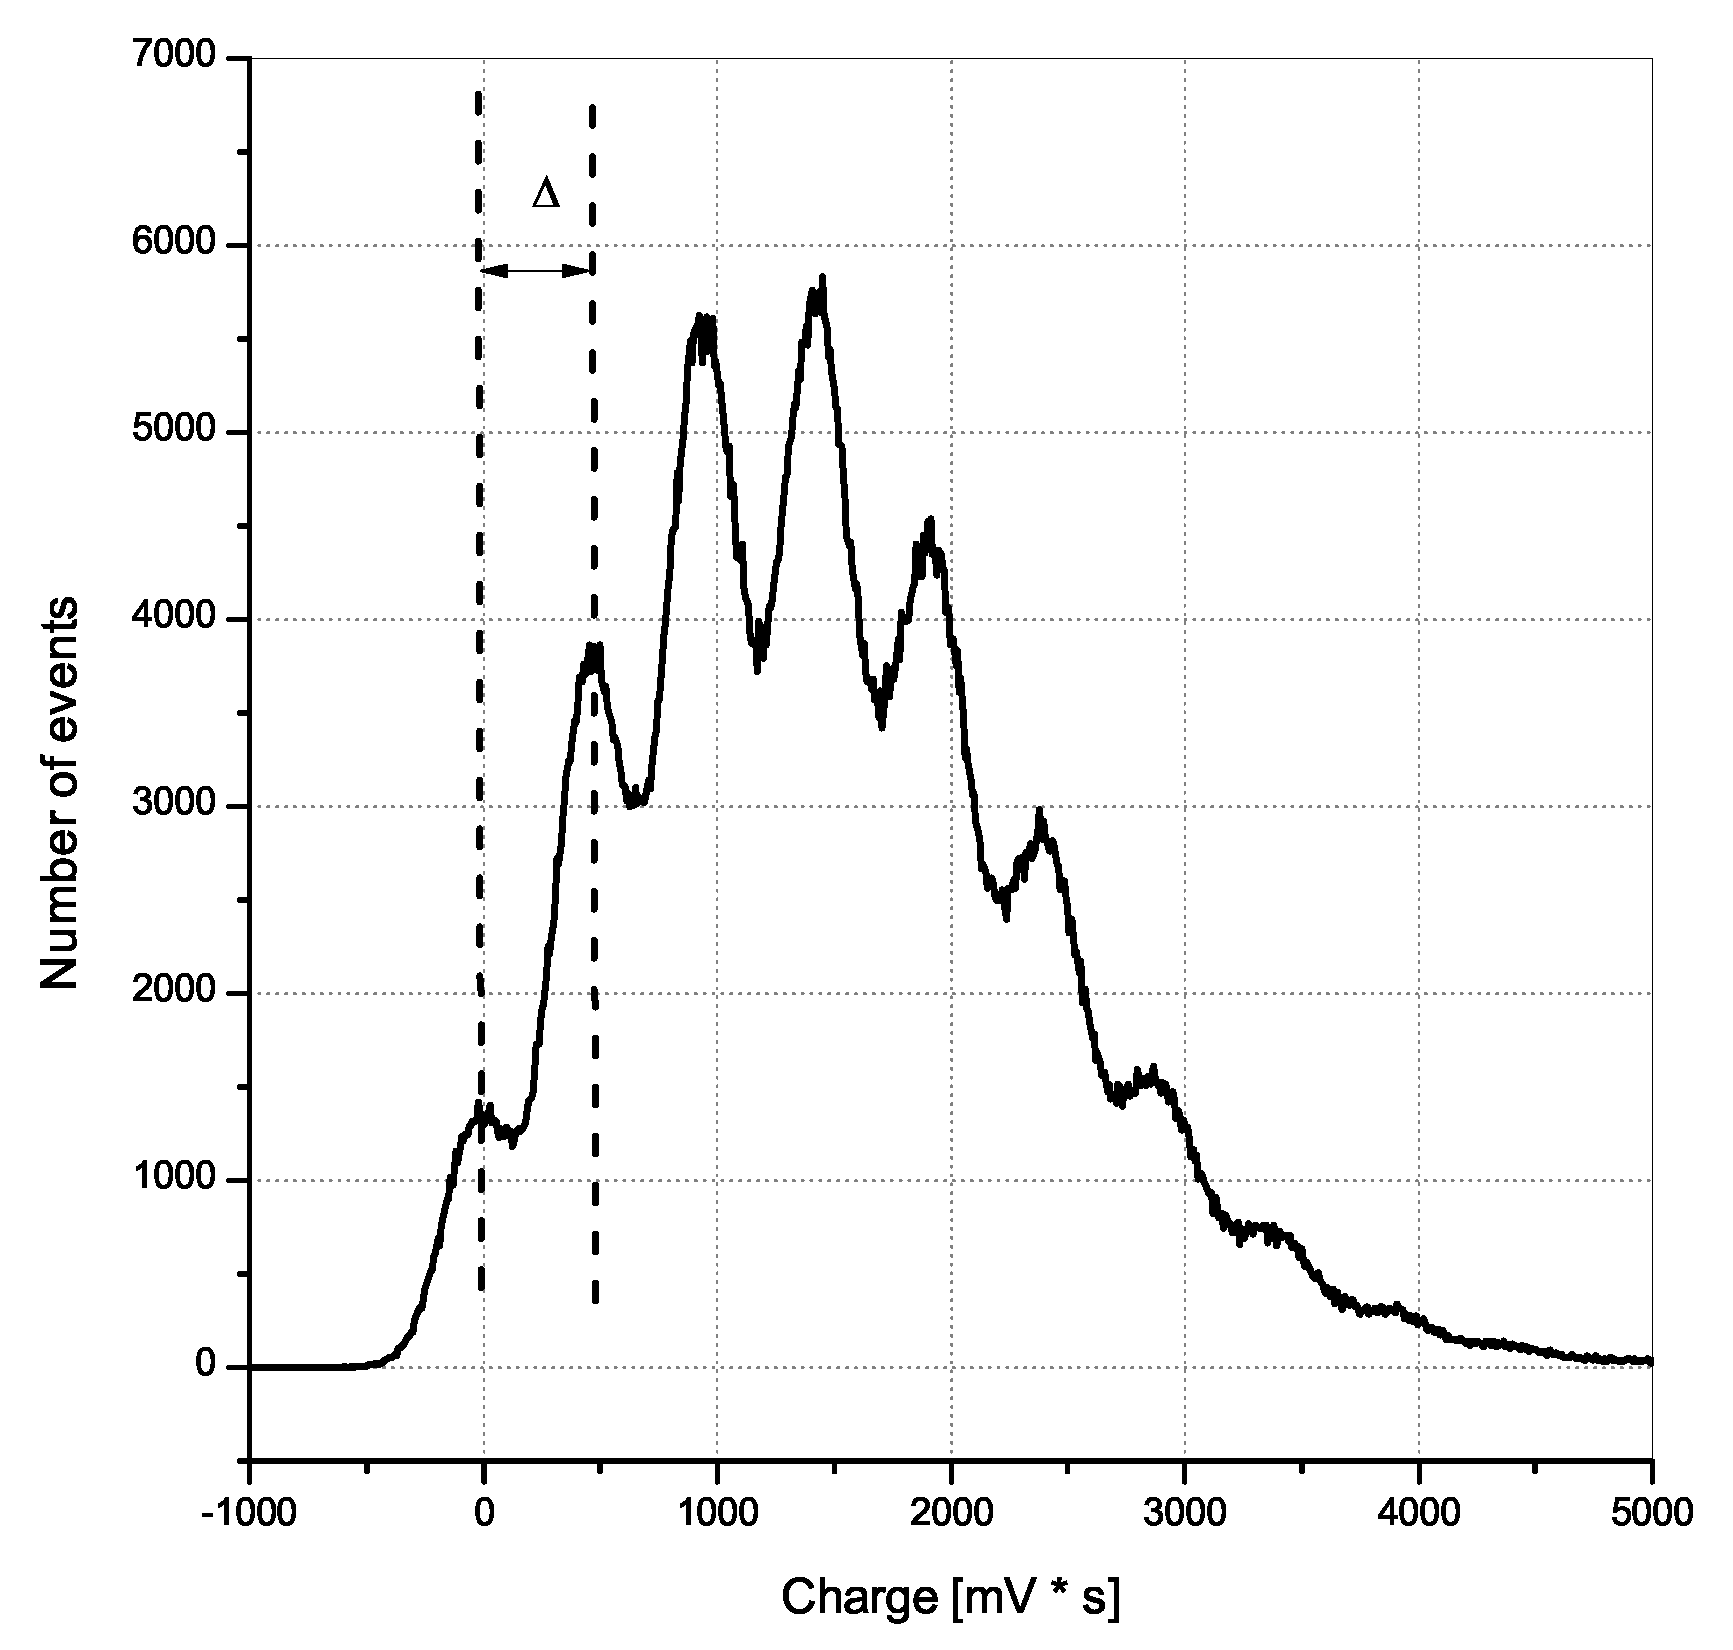
\includegraphics[width=8cm]{sipm_spectrum_eng}}
\caption{Spectrum from Hamamatsu S13360-3050CS at 71 V voltage and 270 K temperature under irradiation by LED.
The integration time is 300 ns.}
\label{image:sipm_spectrum}
\end{figure}

The value $\Delta$ associated with a gain as follows:
$$G = \Delta \cdot ADC_{\text{conversion rate}} / \text{charge of electron},$$
where $ADC_{\text{conversion rate}} [C  / (mV \cdot s)] $ - a conversion coefficient.
To determine the conversion coefficient a rectangular pulse from generator was sent to the test input of the amplifier through the capacitance $C = 1 pF$.
After tract calibration all measurements $G(V, T)$ were approximated by Eq.(\ref{eq:G(V, T)}) to find $a$, $b$, $c$ parameters.
Then using Eq.(\ref{eq:V_bd(T)}) we found the dependence of a breakdown voltage on a temperature.

\section{�ross-talk and after-pulsing probabilities finding algorithm}
\subsection{Theory}
There are several algorithms for finding cross-talk probabilities.
One of them is described in \cite{Characterisation Studies of Silicon Photomultipliers}.
The idea is to measure dark noise rate at different thresholds.
A cross-talk probability can be defined as the ratio of the rates with 1.5 photoelectrons(phe) and 0.5 photoelectrons threshold:
\begin{eqnarray}\label{eq:X_talk}
P_{X-talk} = \nu_{1.5 phe} / \nu_{0.5 phe}
\end{eqnarray}
However, this method has a significant disadvantage: after-pulses are indistinguishable from cross-talk if the former above a threshold.
Furthermore, this algorithm does not use information about a signal form, which makes the frequency dependence of the threshold more blurred and
complicates the finding of the $ \nu_{1.5 pe}$ value.

An advanced algorithm should use the information about a waveform.
There are two approaches to signal processing: inverse convolution \cite{Modeling crosstalk in silicon photomultipliers} and an approximation of the original signal \cite{Characterization and Simulation of the Response, After-pulsingandcross-talkinmulti-pixelphotoncounters, Using MPPCs for T2K Fine Grain Detector}.
In this article we decided to use the method of signal approximation, because it is described in more detail in the above works.

In the process of approximation we obtain amplitudes and start times of signals.
Using this information we recover the time constants and probabilities for after-pulses.

After-pulsing is repeated triggering of a cell, which occurs in some time moment after it is triggering.
The reason of after-pulsing is a capture of electrons into traps during an avalanche and their subsequent release after a time interval from a few nanoseconds to several microseconds \cite{Characterisation Studies of Silicon Photomultipliers}.
After triggering of the primary signal a voltage in a cell decreases to a breakdown voltage and then will recover to its original value exponentially:
\begin{eqnarray}\label{eq:V_current}
V(\Delta t) = V_{BD} + \Delta V \cdot (1 - \exp \left( -\Delta t / \tau_{rec} \right)),
\end{eqnarray}
where $V_{BD}$ - a SiPM breakdown voltage, $\Delta V$ - an overvoltage ,$\tau_{rec}$ - a recovery time of a cell.

There are several processes, which may cause of a cell retriggering.
First of all, it is after-pulsing.
Because of different physical mechanisms of electron traps, there are two types of after-pulses:
fast and slow \cite{After-pulsingandcross-talkinmulti-pixelphotoncounters, Using MPPCs for T2K Fine Grain Detector, Characterization and Simulation of the Response}.
Secondly, dark noise may cause of a cell retriggering.
Each of the two processes has exponential time distribution with its own time constant $\tau$:
\begin{eqnarray}\label{eq:f(dt)_afterpulsing}
f(\Delta t) = \frac{1}{\tau} \cdot \exp(-\Delta t / \tau),
\end{eqnarray}
where $\tau$ - an average time elapsing between two pulses when considering only one of the above effects.
Measuring distances between signals we build pulse interval spectrum.
Then we approximate the probability density of the pulse interval by an analytic function.
Function parameters characterize time constants and probabilities of processes leading to the triggering.

Since we are interested in the pulse interval density, it is necessary to know the probability $P(t)$ that on the interval from $0$ to $t$ pulses can't exist and
on the interval from $t$ to $t + \delta t$ must occur one pulse.
If we consider only one exponential process, this probability is $P_{exp}(t) =  \nu \cdot e^{- t \cdot \nu} \cdot \delta t$ ($t = 1 / \nu$).

We deduce the pulse interval density, if dark pulses or after-pulses can occur in a cell.
For a start, consider the case when there are after-pulses only one type, occurring with a $p$ probability and a $\nu$ frequency.
Dark pulses, as well as after-pulses have an exponential distribution (\ref{eq:f(dt)_afterpulsing}).
Since dark pulses are independent of after-pulses the required probability $P(t)$ can be written as follows:

\begin{eqnarray}\label{eq:probability_dt_simple}
P(t) = P\{ \text{there are not after-pulses from $0$ to $t + \delta t$} \}
\cdot P\{ \text{there is dark pulse from $t$ to $t + \delta t$} \} +  \\ \nonumber
P\{ \text{there is after-pulse from $t$ to $t + \delta t$} \}
\cdot P\{\text{there are not dark pulses from $0$ to $t + \delta t$} \}
\end{eqnarray}

The contribution of each process is as follows:
\begin{eqnarray}\label{eq:probability_dt_simple_parts}
P\{ \text{there are not after-pulses from $0$ to $t + \delta t$} \} = (1 - p) + p \cdot e^{- \nu \cdot t} \\ \nonumber
P\{ \text{there is dark pulse from $t$ to $t + \delta t$} \} = (\nu_{dc} \cdot e^{- \nu_{dc} \cdot t}) \cdot \delta t \\ \nonumber
P\{ \text{there is after-pulse from $t$ to $t + \delta t$} \} = p \cdot ( \nu \cdot e^{- \nu \cdot t} ) \cdot \delta t  \\ \nonumber
P\{\text{there are not dark pulses from $0$ to $t + \delta t$} \} = e^{- \nu_{dc} \cdot t} \\ \nonumber
\end{eqnarray}

Thus, substituting probabilities in Eq.(\ref{eq:probability_dt_simple}) from Eq.(\ref{eq:probability_dt_simple_parts}) and reducing the resulting expression on $\delta t$ we obtain the probability density of pulse intervals:
\begin{eqnarray}\label{eq:probability_dt_fast}
f(t) = p \cdot (\nu + \nu_{dc}) \cdot e^{-(\nu + \nu_{dc}) \cdot t} + (1 - p) \cdot \nu_{dc} \cdot e^{-\nu_{dc} \cdot t}
\end{eqnarray}
It is worth noting that a similar formula is given in \cite{Using MPPCs for T2K Fine Grain Detector}, but with a typo in the sign between the terms.

As a result, taking into account the fast and slow component of after-pulses and dark noise the probability density distribution of pulse intervals can be written as follows:
\begin{eqnarray}\label{eq:dt_probability_fast_slow}
f(t) = p_{s} \cdot p_{f} \cdot (\nu_{s} + \nu_{f} + \nu_{dc} ) \cdot e^{- (\nu_{s} + \nu_{f} + \nu_{dc}) \cdot t} + \\ \nonumber
p_{s} \cdot (1 - p_{f}) \cdot (\nu_{s} + \nu_{dc}) \cdot e^{- (\nu_{s} + \nu_{dc}) \cdot t} + \\ \nonumber
p_{f} \cdot (1 - p_{s}) \cdot (\nu_{f} + \nu_{dc}) \cdot e^{- (\nu_{f} + \nu_{dc}) \cdot t} + \\ \nonumber
(1 - p_{s}) \cdot (1 - p_{f}) \cdot \nu_{dc} \cdot e^{- \nu_{dc} \cdot t}
\end{eqnarray}

Eq.(\ref{eq:dt_probability_fast_slow}) is valid if the measured distance between the signals caused by the triggering of a single cell.
Signals caused by the simultaneous triggering of two or more cells (because of cross-talk) should not be considered in obtaining the probability density of pulse intervals.

In the article \cite{After-pulsingandcross-talkinmulti-pixelphotoncounters} shown another result for the probability density of pulse intervals which differ from that obtained in this work.
This is due to the consideration of one more process - delayed crosstalk.
However, in practice the probability of delayed crosstalk is much lower than the probability of direct cross-talk, and in our experiments we did not observe it.
The information about other processes that are responsible for a cell triggering can be found in \cite{Modeling crosstalk and afterpulsing in siliconphoto multipliers}.

\subsection{Signal finder}

An installation scheme for recording SiPM signals is shown in Fig.\ref{image:install_V_bd_22}.

\begin{figure}[h]
\center{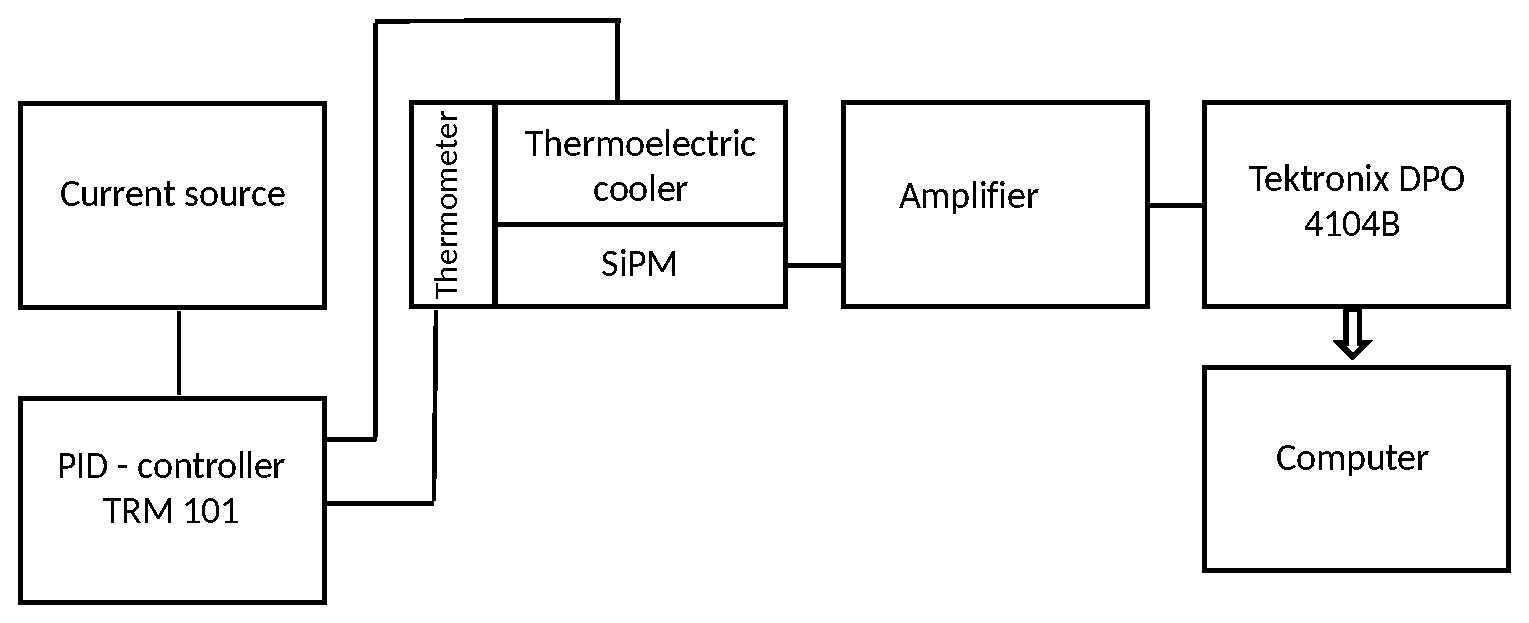
\includegraphics[width=8cm]{install_V_bd_22}}
\caption{The installation scheme for recording SiPM signals.}
\label{image:install_V_bd_22}
\end{figure}


Data in raw format were recorded on a computer using the oscilloscope Tektronix DPO 4104B.
The trigger was disabled during the recording.
The continuous recording length was 5MSamples at a digitizing frequency equal to 5GHz.
For each voltage and temperature on SiPM were recorded 1000 files, i.e. one second of a signal.

The signal from the SiMP can be presented as the sum of single-electron pulses $Signal_{1e}(t - t_{i})$ with a random amplitude $A_{i}$ and a start time $t_{i}$:
\begin{eqnarray}\label{eq:parsing}
V(t) = \sum \limits_{i = 0}^{N} A_{i} \cdot Signal_{1e}(t - t_{i}) + V_{0}
\end{eqnarray}

The waveform of the single-electron pulse was found from the analysis of the recorded signal and was approximated by an analytical function.
The recorded signal was processed by a special algorithm that found single-electron pulses without after-pulses impurities and averaged them.
Signals with after-pulses were thrown out in order to find the correct waveform.
The waveform of the single-electron pulse for different SiPM is shown in Fig.\ref{image:signal_form_comparison}.
The waveform was measured at different overvoltages and temperatures (from -8 to 27 $^{\circ}C$), but one remained practically unchanged.

\begin{figure}[h]
\center{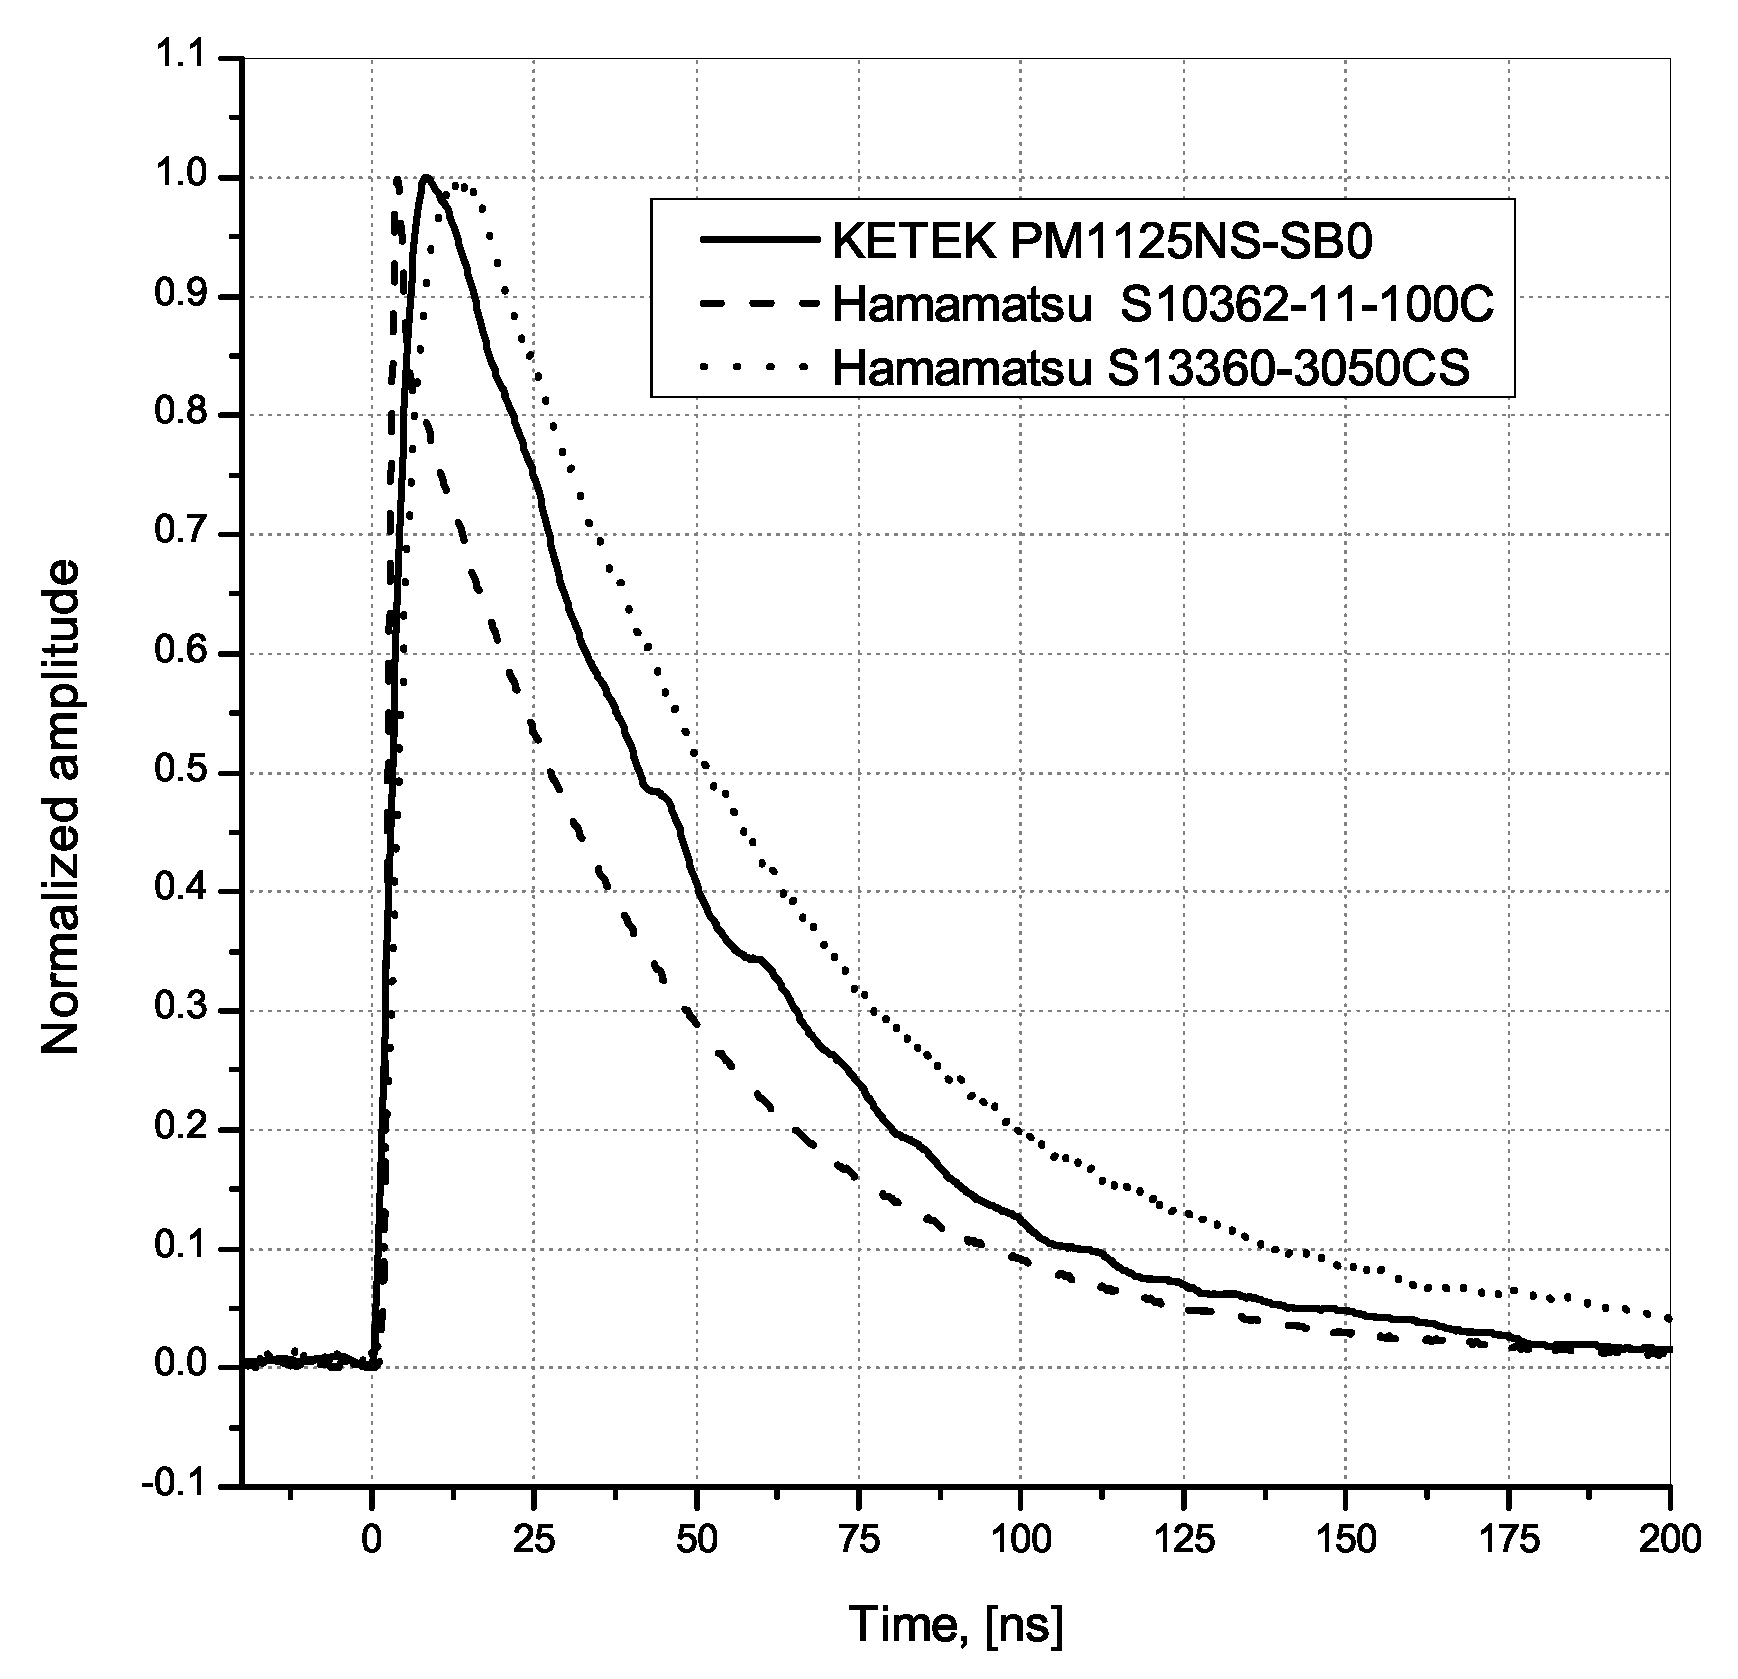
\includegraphics[width=8cm]{signal_form_comparison}}
\caption{The waveform of the single-electron pulse from different SiPMs.}
\label{image:signal_form_comparison}
\end{figure}

Further, single-electron pulses were approximated by function obtained from the convolution of Eq.(\ref{eq:V(t)_base}) with a Gauss distribution describing the contribution of the limited operating speed of electronics.
The Result of a convolution is shown in Eq.(\ref{eq:V(t)_conv}), where $\sigma$ is the standard deviation of the Gauss distribution.

\begin{eqnarray}\label{eq:V(t)_base}
V(t) = A \cdot \exp \left[- \frac{t - t_0}{\tau_{rec}} \right] \cdot \left( 1 - \exp \left[ -\frac{t - t_0}{\tau_{rise}} \right] \right) \cdot \theta(t - t_0) + V_0,
\end{eqnarray}
where $A$ - a pulse amplitude, $t_0$ - a time delay, $\tau_{rec}$ - a recovery time of a cell,
$\tau_{rise}$ - a rise time of a rising edge, $V_0$ - a voltage shift, $\theta(t - t_0)$ - the Heaviside step function.

\begin{eqnarray}\label{eq:V(t)_conv}
V(t) = V_0 + \frac{A}{2} \cdot \Bigg( \left\{ F(\sigma, \tau_{rec}) - F(\sigma, \tau_{total}) \right\} \Bigg), \text{ where} \\ \nonumber
F(\sigma, \tau) = \exp\left[ \frac{\sigma^2 - 2 t \cdot \tau}{2 \tau^2 } \right] \cdot \left( 1 + Erf \left[ \frac{t - \sigma^2 / \tau}{ \sigma \sqrt{2} } \right] \right), \\ \nonumber
\tau_{total} = \frac{\tau_{rec} \cdot \tau_{rise}}{\tau_{rec} + \tau_{rise}}
\end{eqnarray}

A further task was to find $A_{i}$, $t_{i}$ parameters as well as the $N$ parameter.
The $N$ parameter characterizes the number of signals are represented in a data fragment.
A file can be divided into multiple independent parts, each of which describes a signal according to the Eq.(\ref{eq:parsing}) at different $N$ parameters.
A C ++ program was written to process raw data.

The main problem with processing is the presence of noise.
There are a lot of digital filters that can smooth a signal, but their use will lead to loss of the information about after-pulses.
After-pulses are exponentially distributed in time and with a high probability they occur at short times, when a cell voltage has not yet recovered.

However, an accuracy of signals location can be improved if we transmit into the approximation algorithm initial parameters close to true ones.
For this purpose a signal derivative was calculated with the simultaneous smoothing (The Savitsky-Golay third-order filter with the number of points equal to 51 (10.2 ns) )
Thus, the information about the derivative was also involved in the processing.

To split a recorded file into multiple independent signals, we used the following algorithm: \\
1) The first derivative was calculated using the Savitsky-Golay filter. \\
2) If the derivative and an amplitude was higher of threshold values $th_{der}$ and $th_{amp}^{start}$ then the time 20 ns before this event was taken as the time of the start signal.
This condition was necessary for the proper calculation of a basic line of a signal.
Otherwise, a falling edge from a previous signal distort the baseline. \\
3) If after the previous step passed more than 5 ns and the signal level was below the threshold amplitude $th_{amp}^{stop}$ and
ahead on 20 ns the derivative was below the threshold $th_{der}$, then this time was the end time of the signal.
The amplitude threshold $th_{amp}^{stop}$ was chosen as the intersection of the signal with the baseline.

To determine $th_{amp}^{start}$ we drew the dependence of events number from the threshold at different values of the dead time $\tau_{amp}^{dead}$.
An example is shown in Fig.~\ref{image:Hamamatsu_S10362-11-100C_295K_1OV_amp_th} for Hamamatsu S10362-11-100C at $T = 295K$ and $\Delta V = 1 V$.
The threshold for triggering by amplitude $th_{amp}^{start}$ was chosen at half amplitude of the single-electron signal and corresponded approximately to $0.02V$
The thresholds was practically independent of the selected dead time $\tau_{amp}^{dead}$.

A similar graph can be drawn for the derivative (Fig.~\ref{image:Hamamatsu_S10362-11-100C_295K_1OV_der_th}).
We selected only those signals that exceed the amplitude threshold $th_{amp}^{stop} = 0.002V$.
Without this condition the graph would be significantly distorted because noise can have a derivative is comparable to a signal derivative.
Above the threshold $4 \cdot 10^{-4} V / s$  the contribution of noise is significantly suppressed.
This value is selected as $th_{der}$.
However, thresholds $th_{der}$ and $th_{amp}^{start}$ are other for other overvoltages.

\begin{figure}[h]
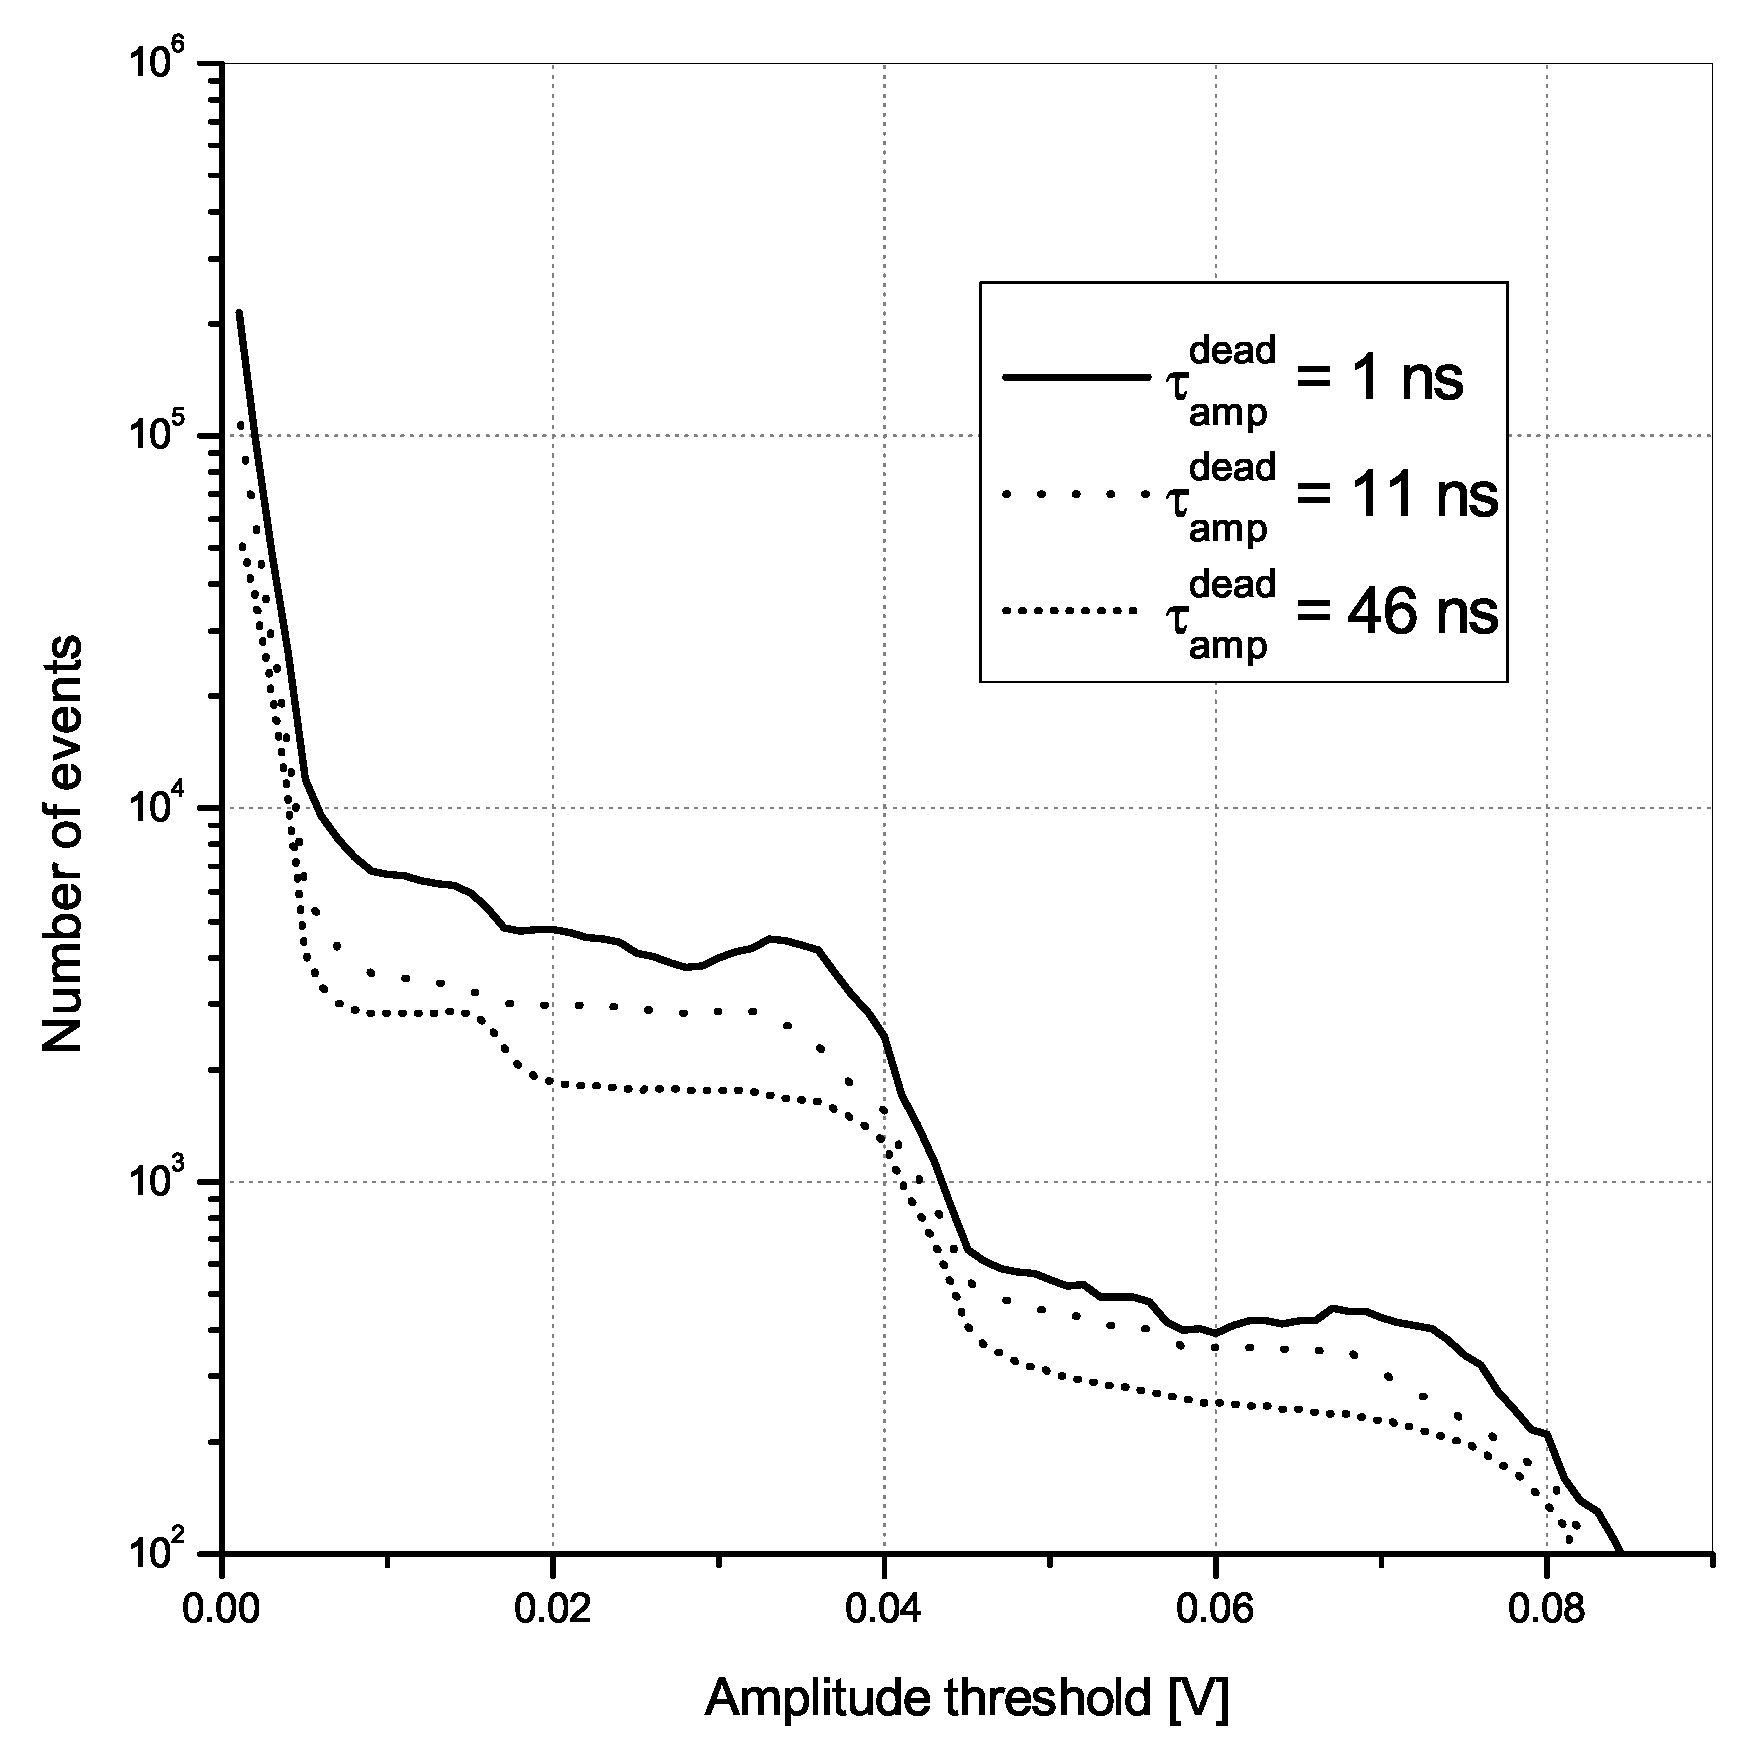
\includegraphics[width=0.47\textwidth]{Hamamatsu_S10362-11-100C_295K_1OV_amp_th_eng}
\hfill
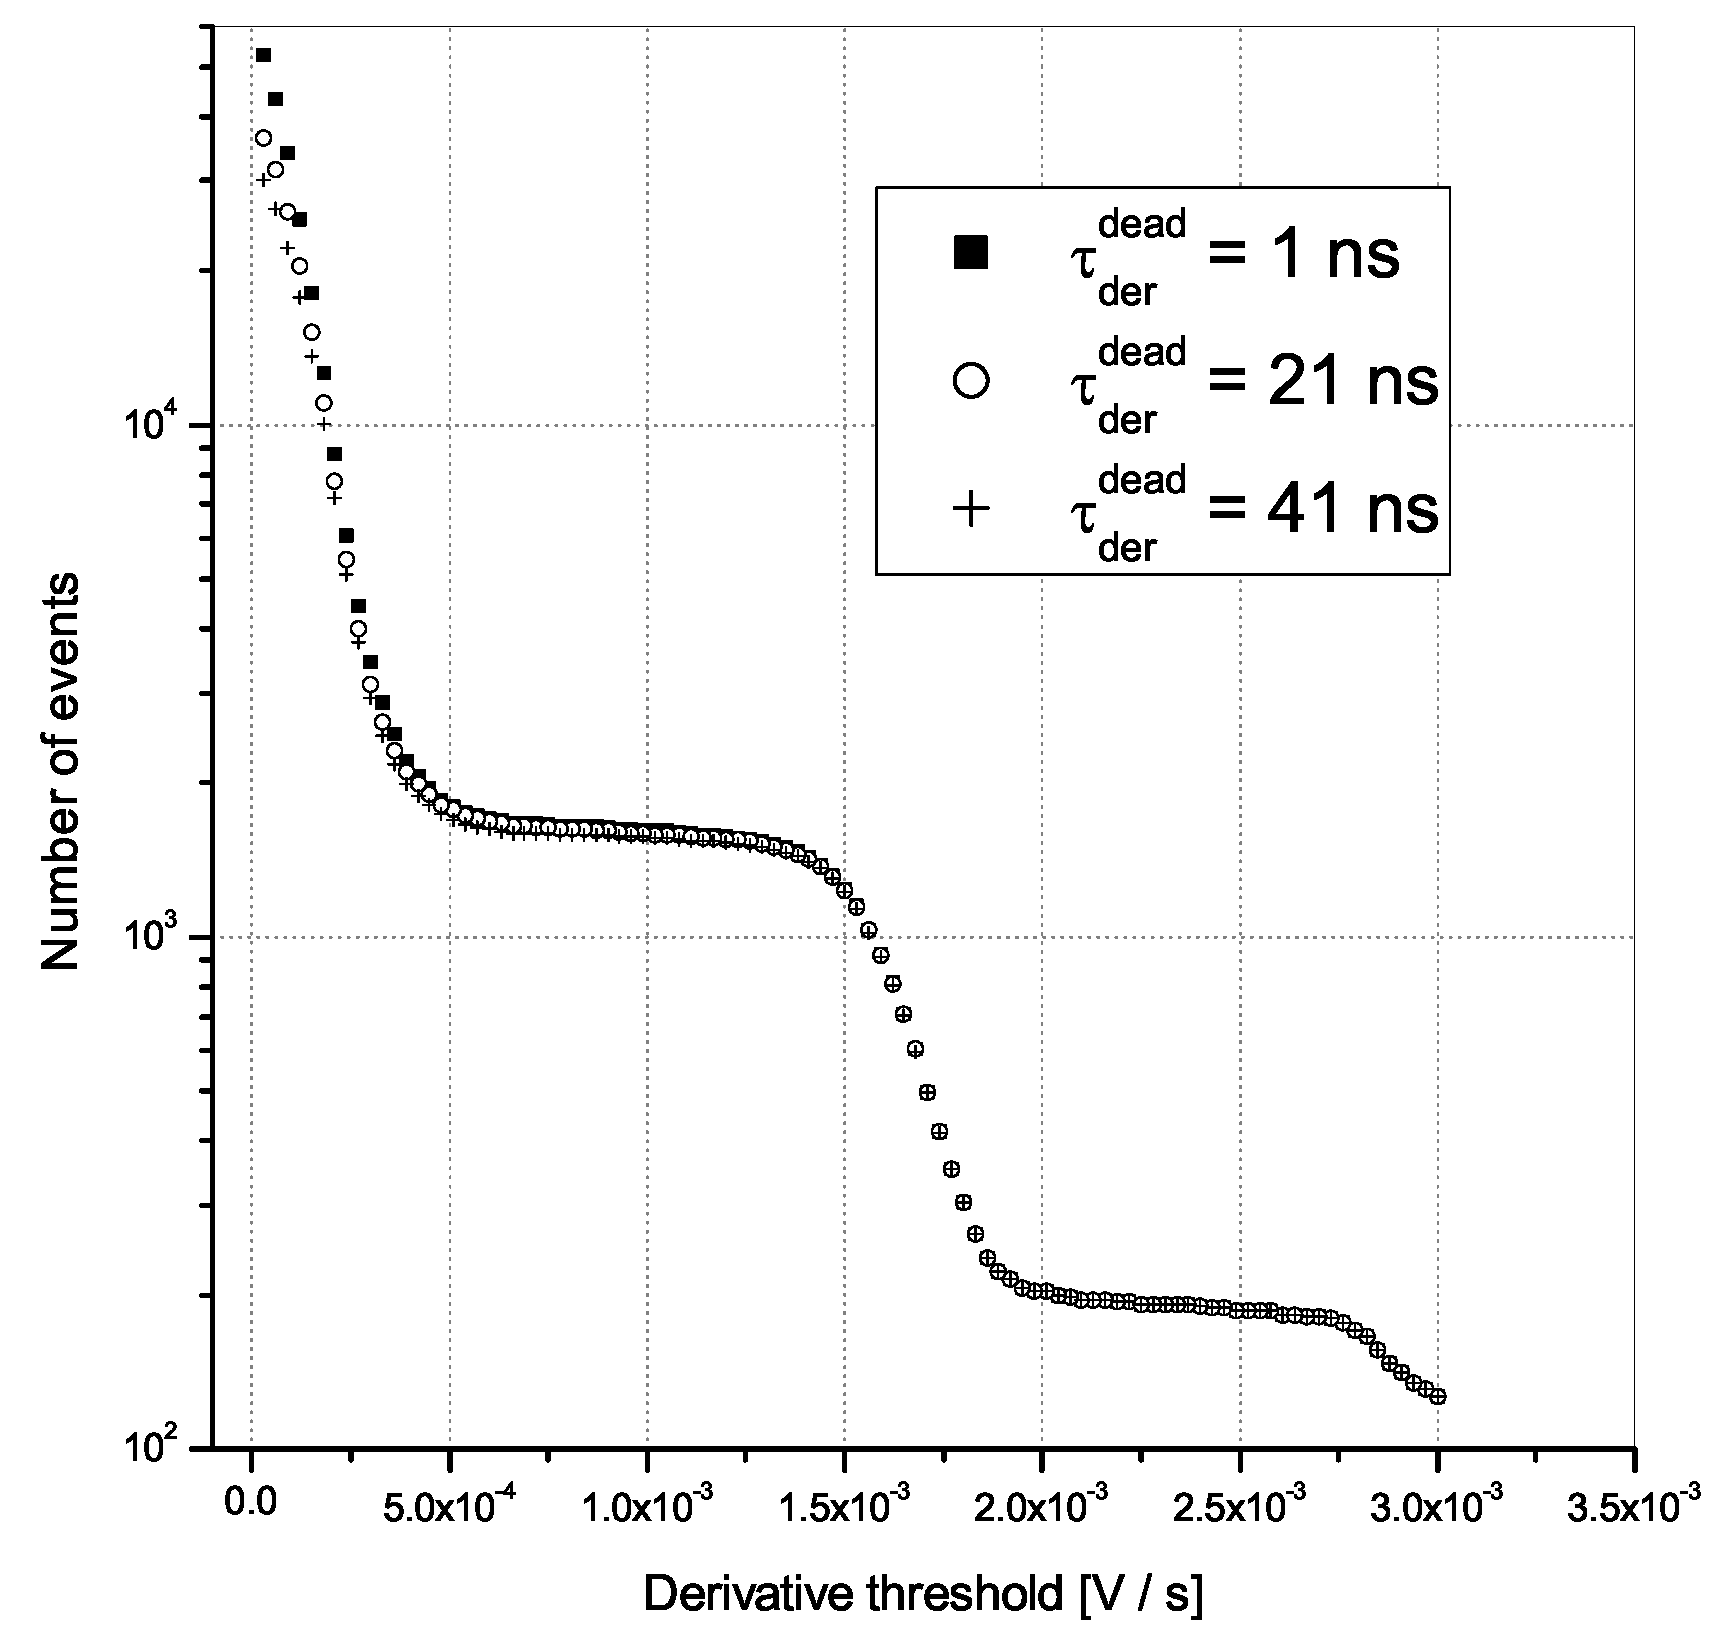
\includegraphics[width=0.47\textwidth]{Hamamatsu_S10362-11-100C_295K_1OV_der_th_eng}
\\
\parbox[t]{0.47\textwidth}{\caption{The dependence of the number of found signals from the amplitude threshold and the dead time $\tau_{amp}^{dead}$ for
Hamamatsu S10362-11-100C at 1V overvoltage and 295K temperature.}
\label{image:Hamamatsu_S10362-11-100C_295K_1OV_amp_th}}
\hfill
\parbox[t]{0.47\textwidth}{\caption{The dependence of the number of found signals from the derivative threshold and the dead time $\tau_{der}^{dead}$ for
Hamamatsu S10362-11-100C at 1V overvoltage and 295K temperature. Only signals exceeding the threshold $th_{amp}^{stop} = 0.002 V /s$ were selected.}
\label{image:Hamamatsu_S10362-11-100C_295K_1OV_der_th}}
\end{figure}

As a result of this algorithm data files were divided into multiple independent parts.
At each part can be either one pulse or many pulses.
\subsection{Correlation analysis}

To find parameters $A_{i}$ and $t_{i}$ each part have to be approximated by Eq.(\ref{eq:parsing}).
This function internally nonlinear on the $t_{i}$ parameter therefore it is necessary to set the initial parameter of the start time of a signal.
To do this, we used the following algorithm:\\
1) If the first derivative was above the threshold, then we were looking for a derivative maximum from a current time to a current time plus 5 ns.
The time at which the first derivative reached the maximum used as the initial value of the $t_{i}$ parameter.\\
2) If the first derivative was below the threshold value and passed more than 5 ns then was allowed to search for the next threshold exceeding.\\

Further, an each independent part was approximated by Eq.(\ref{eq:parsing}) at $N = 1$.
Consider the correlation between the amplitude and $\chi^2 / Dof$ (Fig.~\ref{image:Hamamatsu_S10362-11-100C_295K_1V_Chi2_amp 1}).
One can notice a few outlying clusters: $A_{1}$, $B_{1}$, $C_{1}$ etc.
The cluster $A_{1}$ corresponds to single-electron signals.
Clusters $B_{1}$, $C_{1}$ etc. corresponds to events when simultaneously triggered two, three or more cells (cross-talk), and these signals was located away from other signals.
Because of this they have the low $\chi^2 / Dof$ value at the approximation of a single-component function.
Other events with the $\chi^2 / Dof > 4$ value (we denote them as $Z_{1}$ cluster ) correspond to several signals, located at a relatively short distance distance from other.

In the next step the events from the $Z_{1}$ cluster were approximated by Eq.(\ref{eq:parsing}) at $N = 2$.
In that case, each event is characterized by four parameters: $\chi^2 / Dof $, $amp_{1}$ and $amp_{2}$ - amplitudes of the first and the second signals, $\Delta t$ - a distance between the signals.
Draw a correlation between the total amplitude $amp_{1} + amp_{2}$ and a $\chi^2 / Dof $ value (Fig.~\ref{image:Hamamatsu_S10362-11-100C_295K_1_OV_Chi2_amp1_amp2}).

\begin{figure}[h]
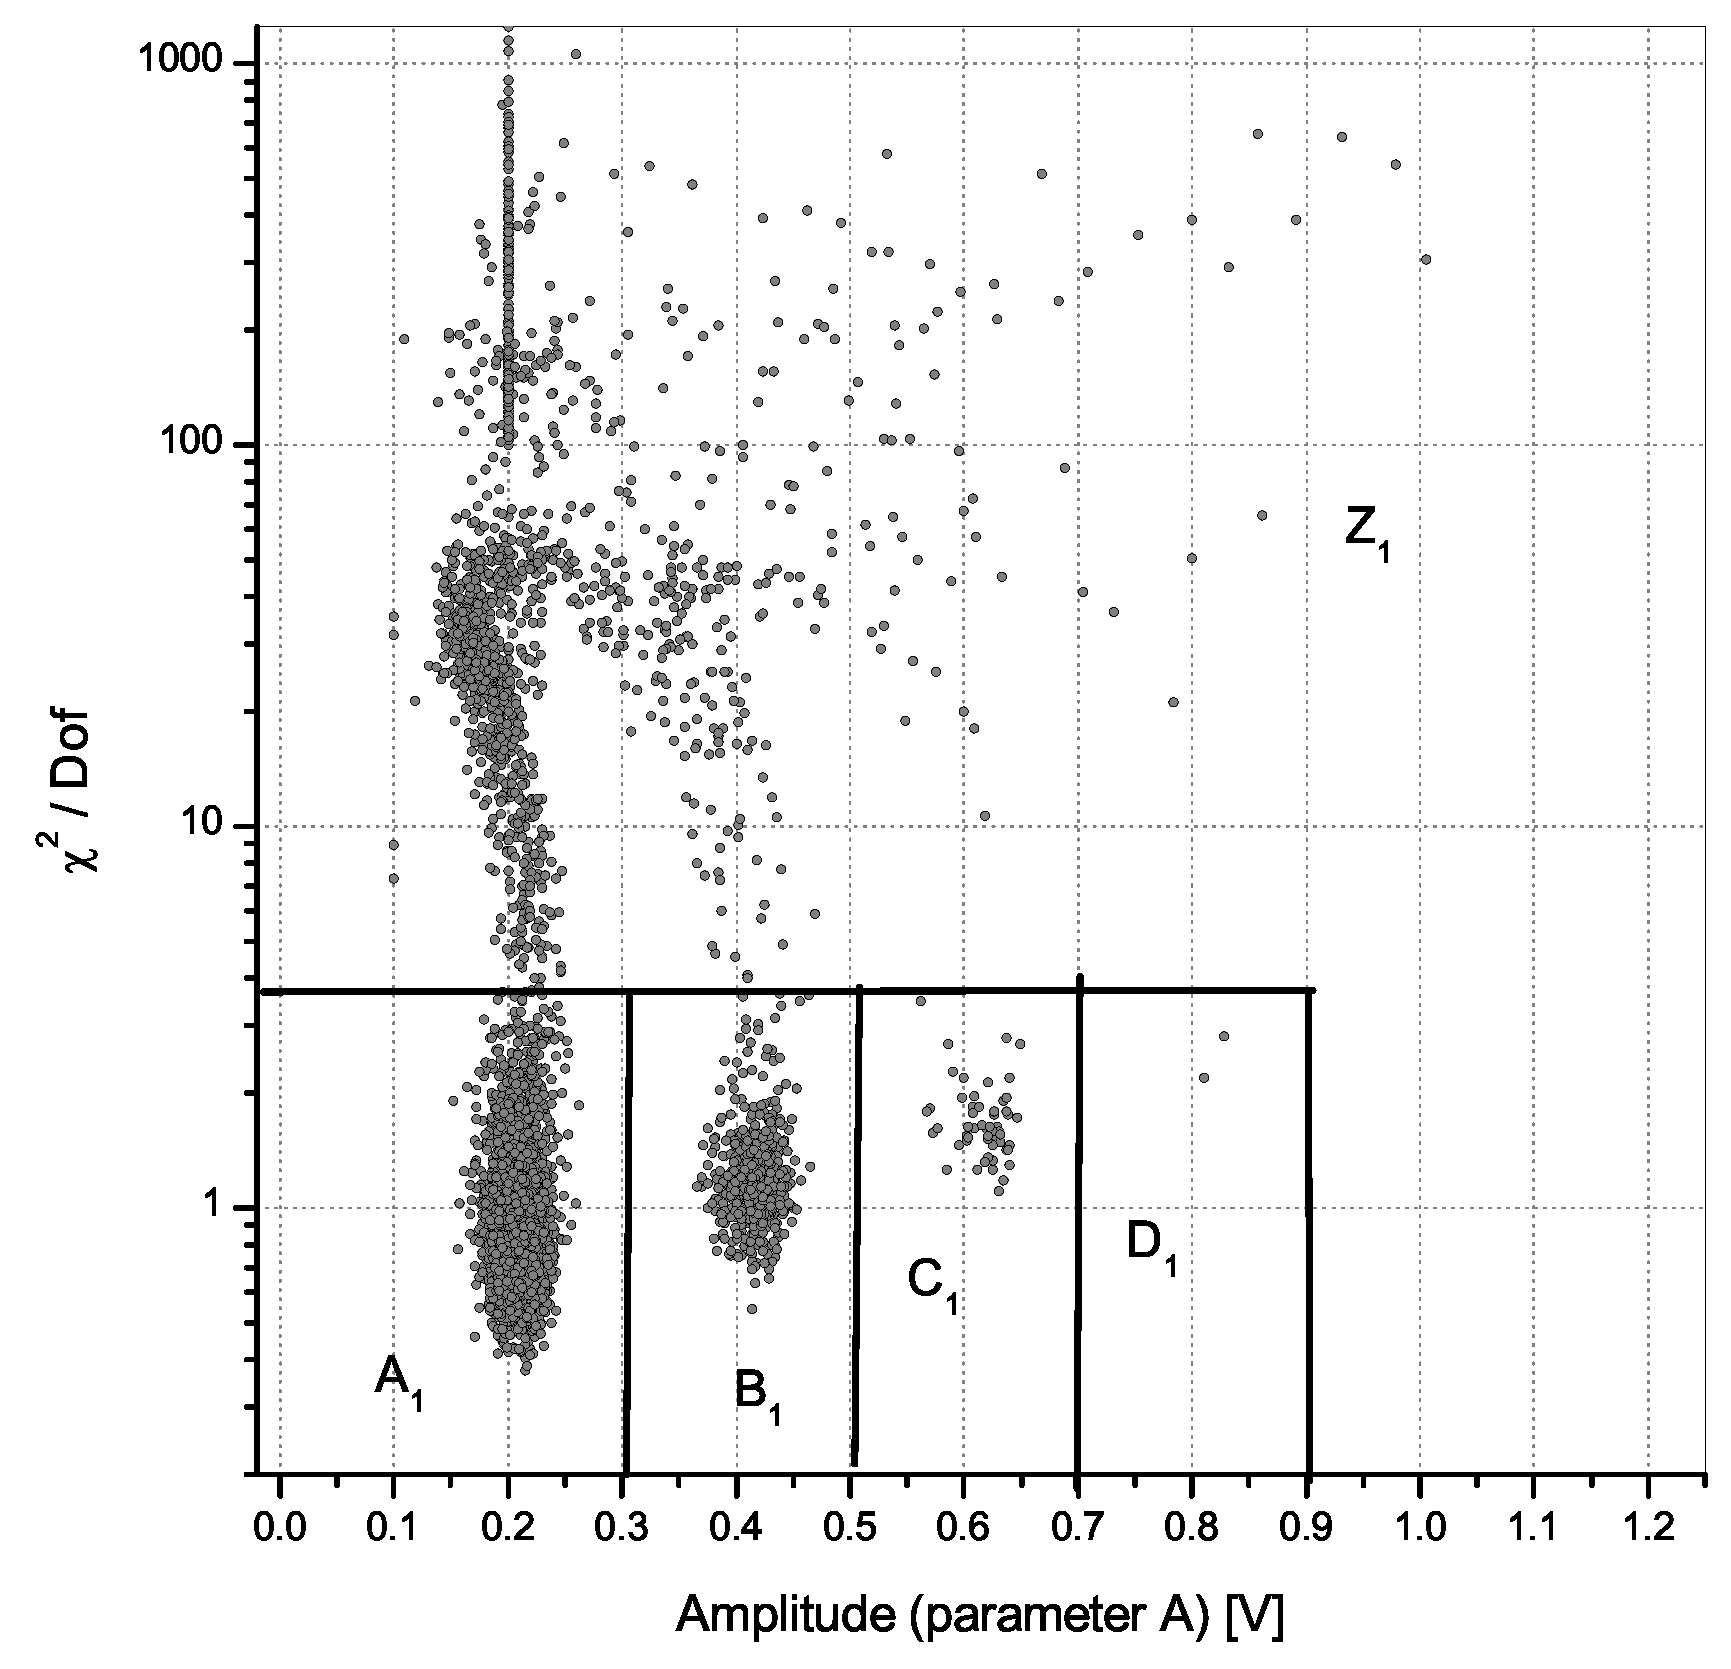
\includegraphics[width=0.47\textwidth]{Hamamatsu_S10362-11-100C_295K_1V_Chi2_amp_1}
\hfill
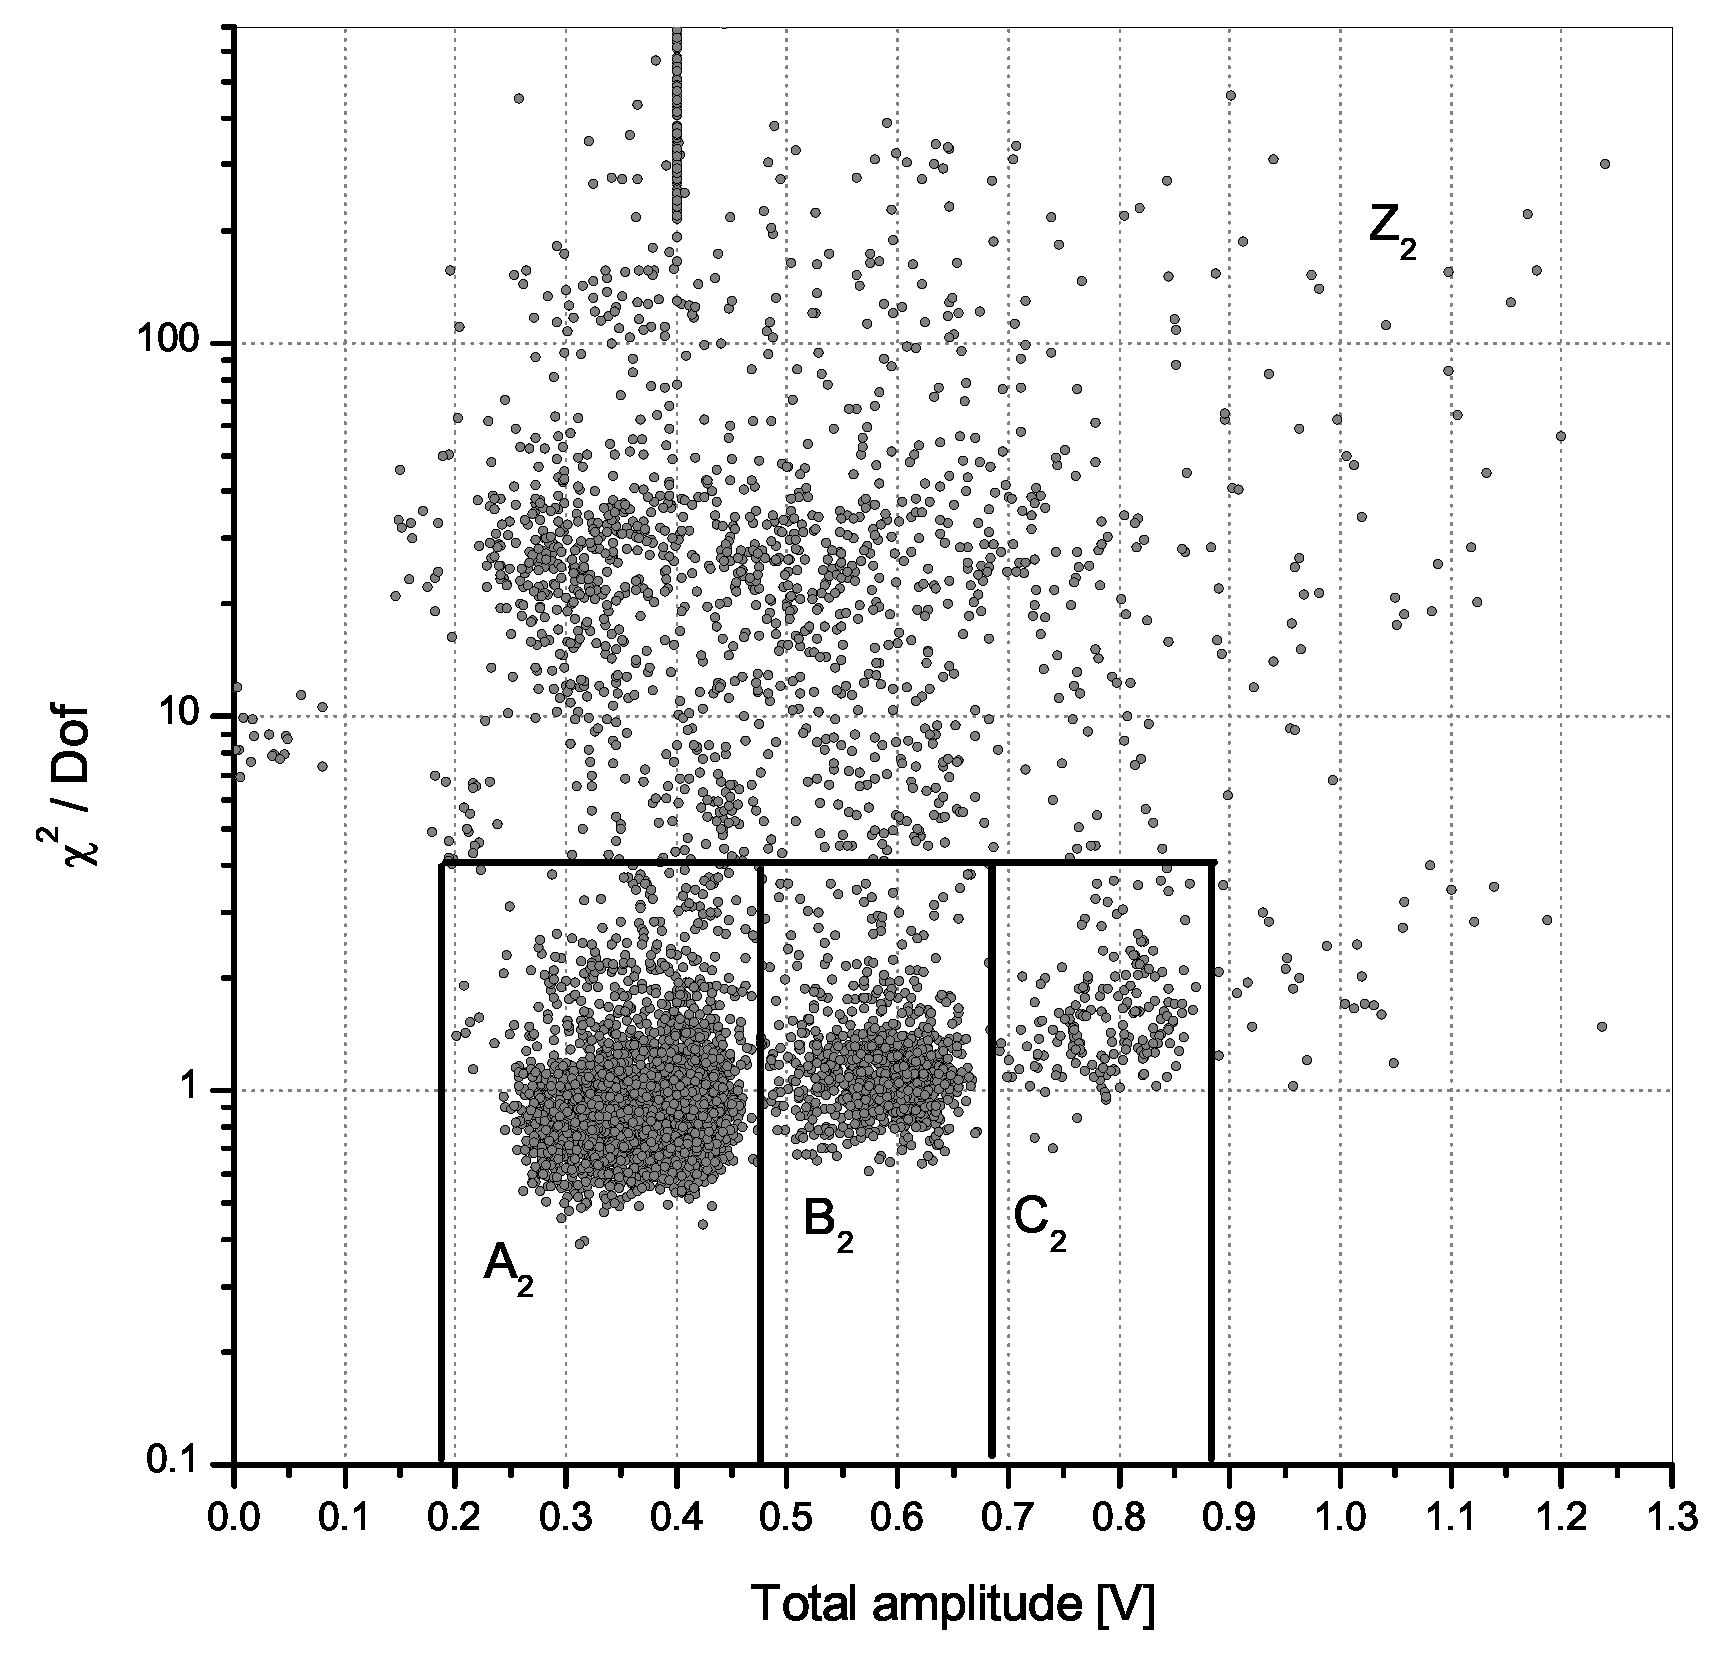
\includegraphics[width=0.47\textwidth]{Hamamatsu_S10362-11-100C_295K_1_OV_Chi2_amp1_amp2_eng}
\\
\parbox[t]{0.47\textwidth}{\caption{The correlation between the total amplitude $amp_{1} + amp_{2}$ and $\chi^2 / Dof$ when approximating all pulses by one-component function.
The signal was obtained from Hamamatsu S10362-11-100C at 1V overvoltage and 295K temperature.}
\label{image:Hamamatsu_S10362-11-100C_295K_1V_Chi2_amp 1}}
\hfill
\parbox[t]{0.47\textwidth}{\caption{The correlation between the total amplitude $amp_{1} + amp_{2}$ and $\chi^2 / Dof$ when approximating the $Z_{1}$ cluster (see Fig.~\ref{image:Hamamatsu_S10362-11-100C_295K_1V_Chi2_amp 1}) by two-component function.
The signal was obtained from Hamamatsu S10362-11-100C at 1V overvoltage and 295K temperature.}
\label{image:Hamamatsu_S10362-11-100C_295K_1_OV_Chi2_amp1_amp2}}
\end{figure}

In this case also there are several typical clusters: $A_{2}$, $B_{2}$, $C_{2}$ etc.
A more clear idea about the signals forming these clusters can be obtained from the correlation of $amp_{1} + amp_{2}$ and $\Delta t$ constructed for a particular cluster (Fig.~\ref{image:Hamamatsu_S10362-11-100C_295K_1_OV_amp1_amp2_dt_A2} and Fig.~\ref{image:Hamamatsu_S10362-11-100C_295K_1_OV_amp1_amp2_dt_B2}).

\begin{figure}[h]
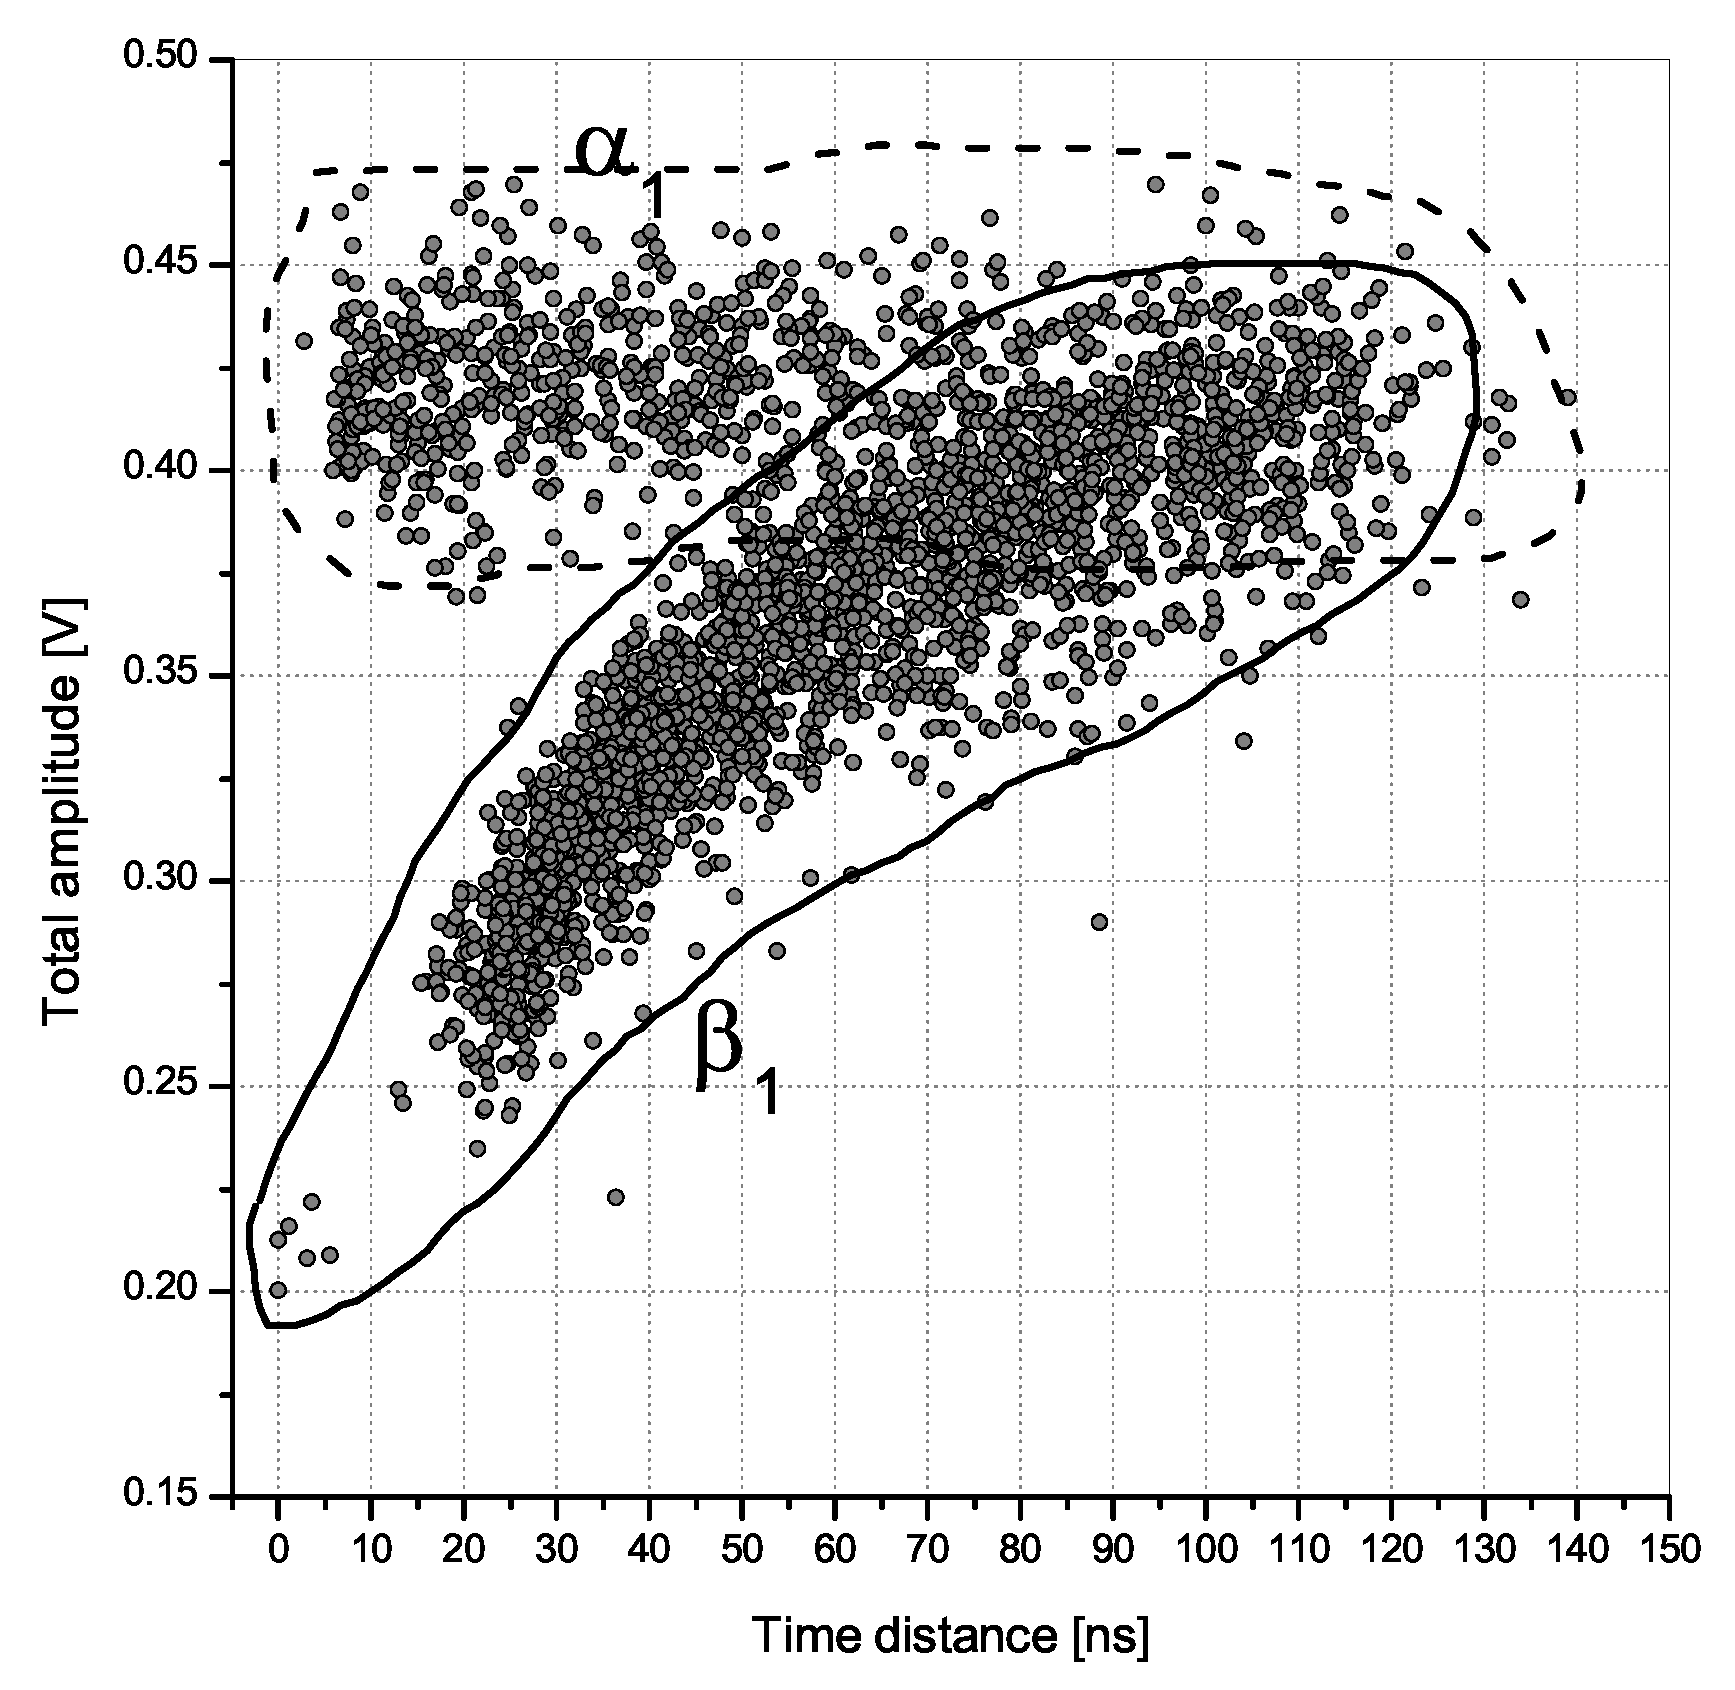
\includegraphics[width=0.47\textwidth]{Hamamatsu_S10362-11-100C_295K_1_OV_amp1_amp2_dt_A2_eng}
\hfill
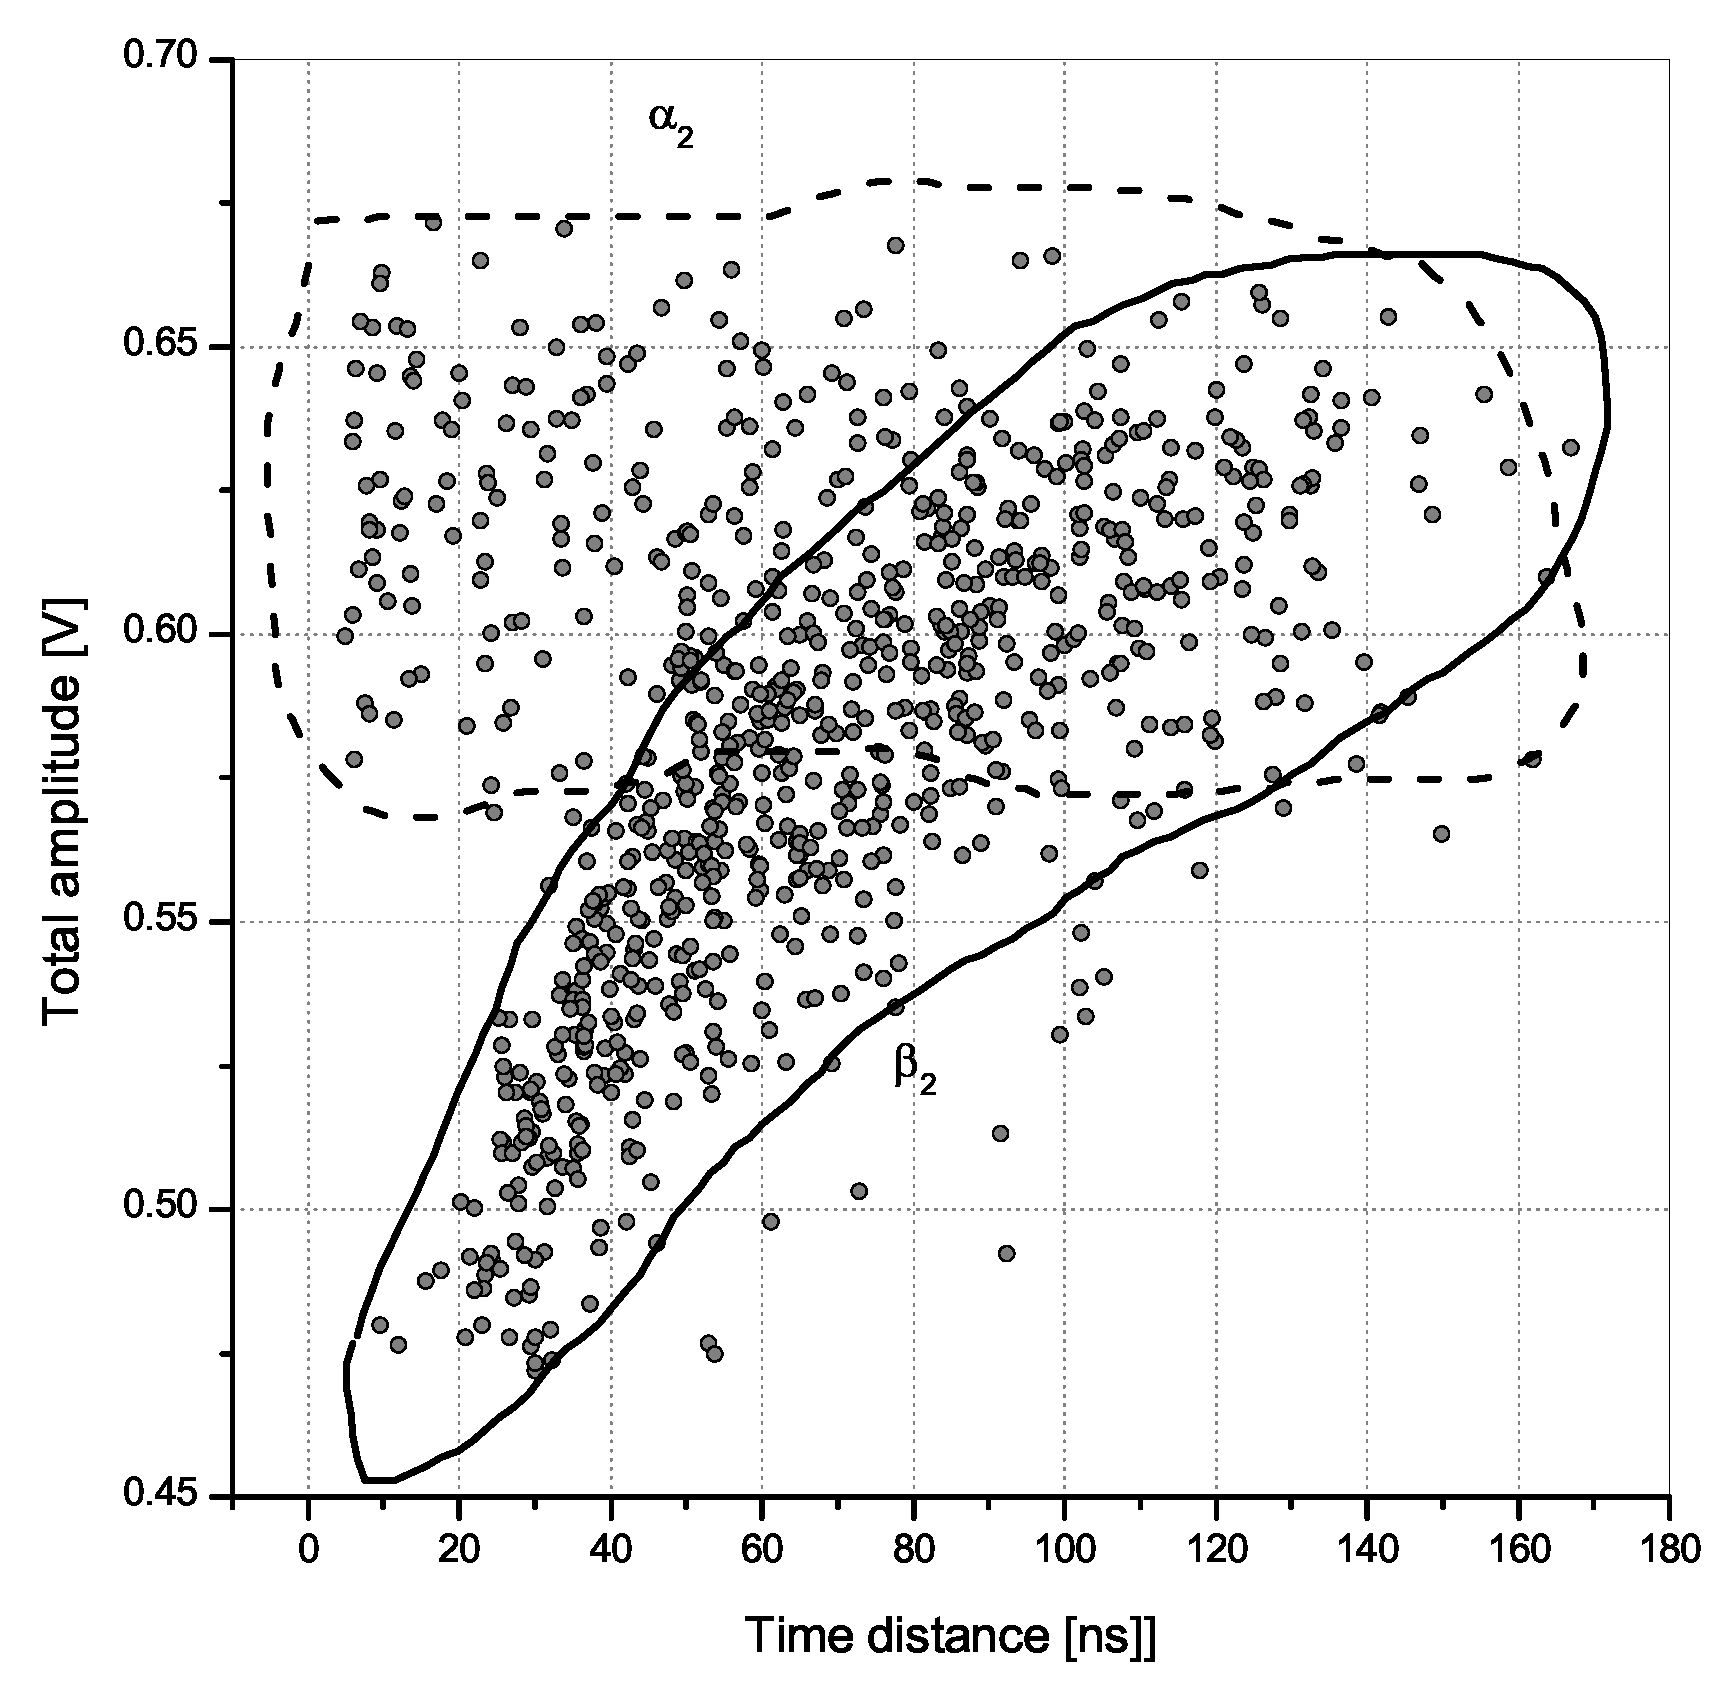
\includegraphics[width=0.47\textwidth]{Hamamatsu_S10362-11-100C_295K_1_OV_amp1_amp2_dt_B2_eng}
\\
\parbox[t]{0.47\textwidth}{\caption{The correlation between the pulse interval and the total amplitude when approximating the $A_{2}$ cluster
(see Fig.~\ref{image:Hamamatsu_S10362-11-100C_295K_1_OV_Chi2_amp1_amp2}) by two-component function.
The signal was obtained from Hamamatsu S10362-11-100C at 1V overvoltage and 295K temperature.}
\label{image:Hamamatsu_S10362-11-100C_295K_1_OV_amp1_amp2_dt_A2}}
\hfill
\parbox[t]{0.47\textwidth}{\caption{The correlation between the pulse interval and the total amplitude when approximating the $B_{2}$ cluster
(see Fig.~\ref{image:Hamamatsu_S10362-11-100C_295K_1_OV_Chi2_amp1_amp2}) by two-component function.
The signal was obtained from Hamamatsu S10362-11-100C at 1V overvoltage and 295K temperature.}
\label{image:Hamamatsu_S10362-11-100C_295K_1_OV_amp1_amp2_dt_B2}}
\end{figure}

The $A{2}$ cluster consists of signals that are conventionally divided into two sets: $\alpha_{1}$ �  $\beta_{1}$.
The set $\alpha_{1}$ corresponds to two closely spaced signals and their total amplitude equal to double amplitude of the single-electron pulse.
This means that these signals were caused by triggering of various cells and they are dark noise.
At the same time signals from the set $\beta_{1}$ have an amplitude that depends on the distance between signals.
This means that the first signal was a single-electron signal and the subsequent signal was an after-pulse.
The similar correlation can be constructed for the $B_{2}$ set (Fig.~\ref{image:Hamamatsu_S10362-11-100C_295K_1_OV_amp1_amp2_dt_B2}).
In this case, the set $\alpha_{2}$ consists of two closely spaced signals one of which has a single-electron amplitude.
Another signal has the double amplitude caused by the simultaneous triggering of two cells due to cross-talk.

The set $\beta_{2}$ contains signals that can be divided into two groups.
The first group was formed by signals in which two cells triggered simultaneously and then one of cells generated an after-pulse.
The second group was formed by signals in which one cell triggered and then after-pulse occurred which caused cross-talk.
The sets similar to $A_{2}$ and $A_{2}$ with a large total amplitude correspond to the events with a greater number of simultaneously triggered cells.

Then we built pulse interval spectrum.
We took into account only the signals without cross-talk, i.e. we measured the distance only between those signals that belong to the $A_{1}$ or $A_{2}$ clusters.
In the first approximation we can neglect events in the $A_{3}$, $A_{4}$ etc. clusters due to their small number relative to events in the $A_{1}$ or $A_{2}$ clusters.

As a result, we obtained the pulse interval spectrum shown in Fig.~\ref{image:Hamamatsu_S10362-11-100C_295K_1_OV_dt_spectrum}.
By approximating the spectrum by Eq.(\ref{eq:dt_probability_fast_slow}) we found $p_{s}$, $p_f$, $\nu_{s}$, $\nu_{f}$, $\nu_{DC}$ parameters.
For the approximation RooFit package and unbinned fit were used.

As you can see there is a change in the spectrum monotony when the pulse interval equals approximately 25 ns.
If the after-pulse occurs with the pulse interval less than 25 ns after the previous pulse, its amplitude is small and this pulse cannot be distinguished from noise.
Because of this the signal is recognized as a single component and it does not contribute to the short times.
This distorts the spectrum.
For the correct approximation we took into account only pulse intervals exceed a certain "threshold" value.
To clarify this value approximation was performed at different threshold values.
The dependence of the $\tau_{f}$ parameter from the pulse interval threshold is shown in Fig.~\ref{image:Hamamatsu_S10362-11-100C 295K_1_OV_dt_spectrum_timecut}.
For this type of SiMP at 295K temperature and 1V overvoltage 25 ns threshold was chosen.
When reducing the overvoltage the pulse interval threshold increases.

\begin{figure}[h]
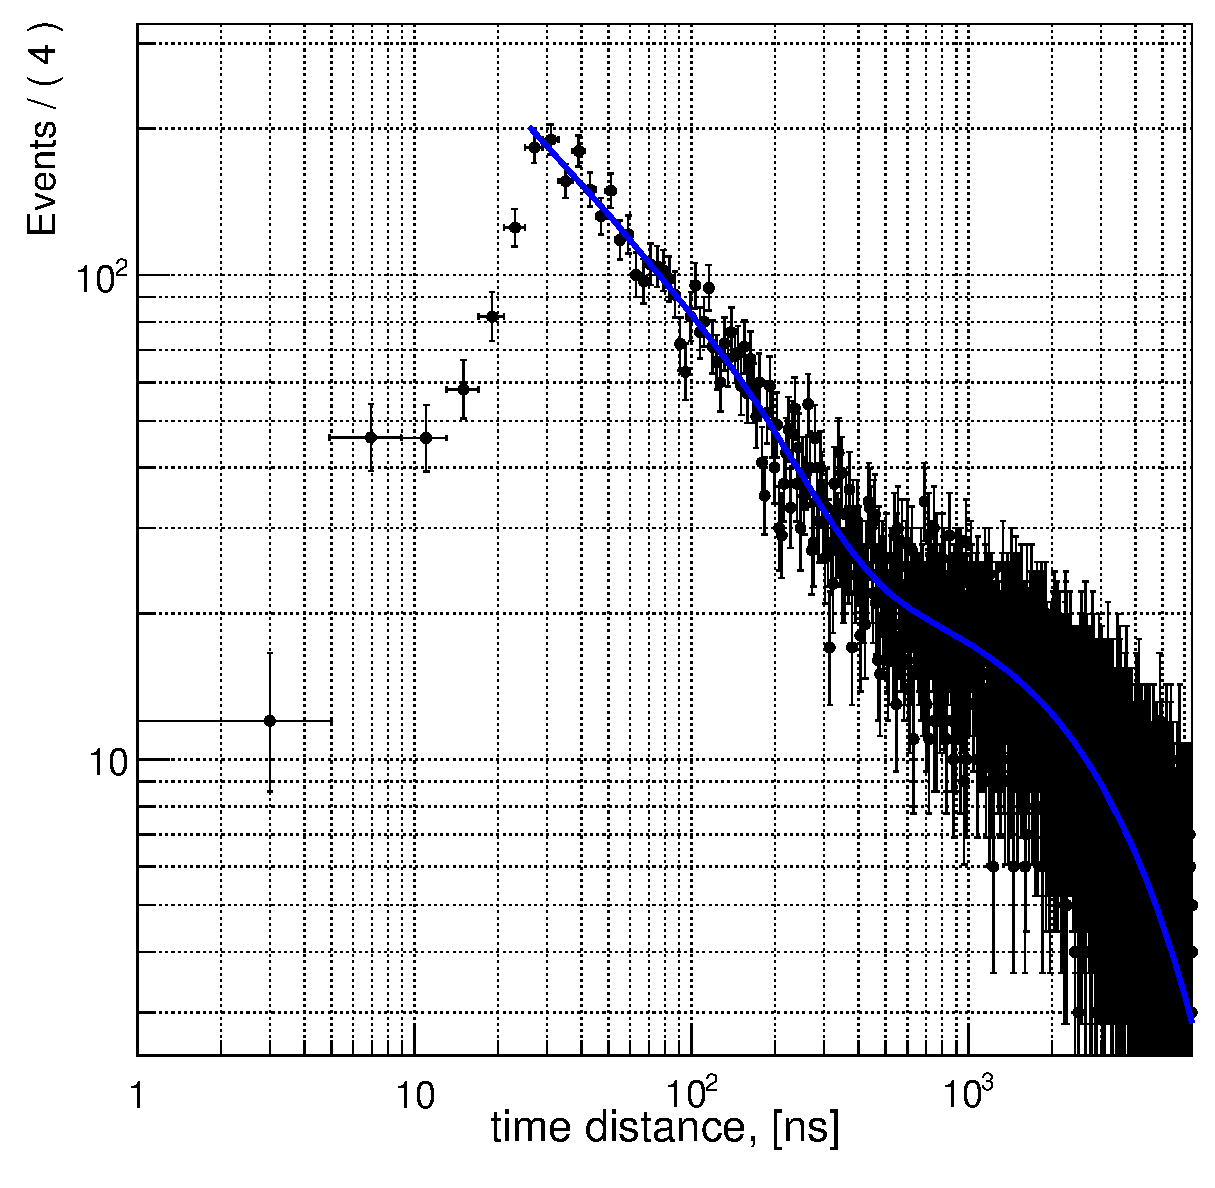
\includegraphics[width=0.47\textwidth]{Hamamatsu_S10362-11-100C_295K_1_OV_dt_spectrum}
\hfill
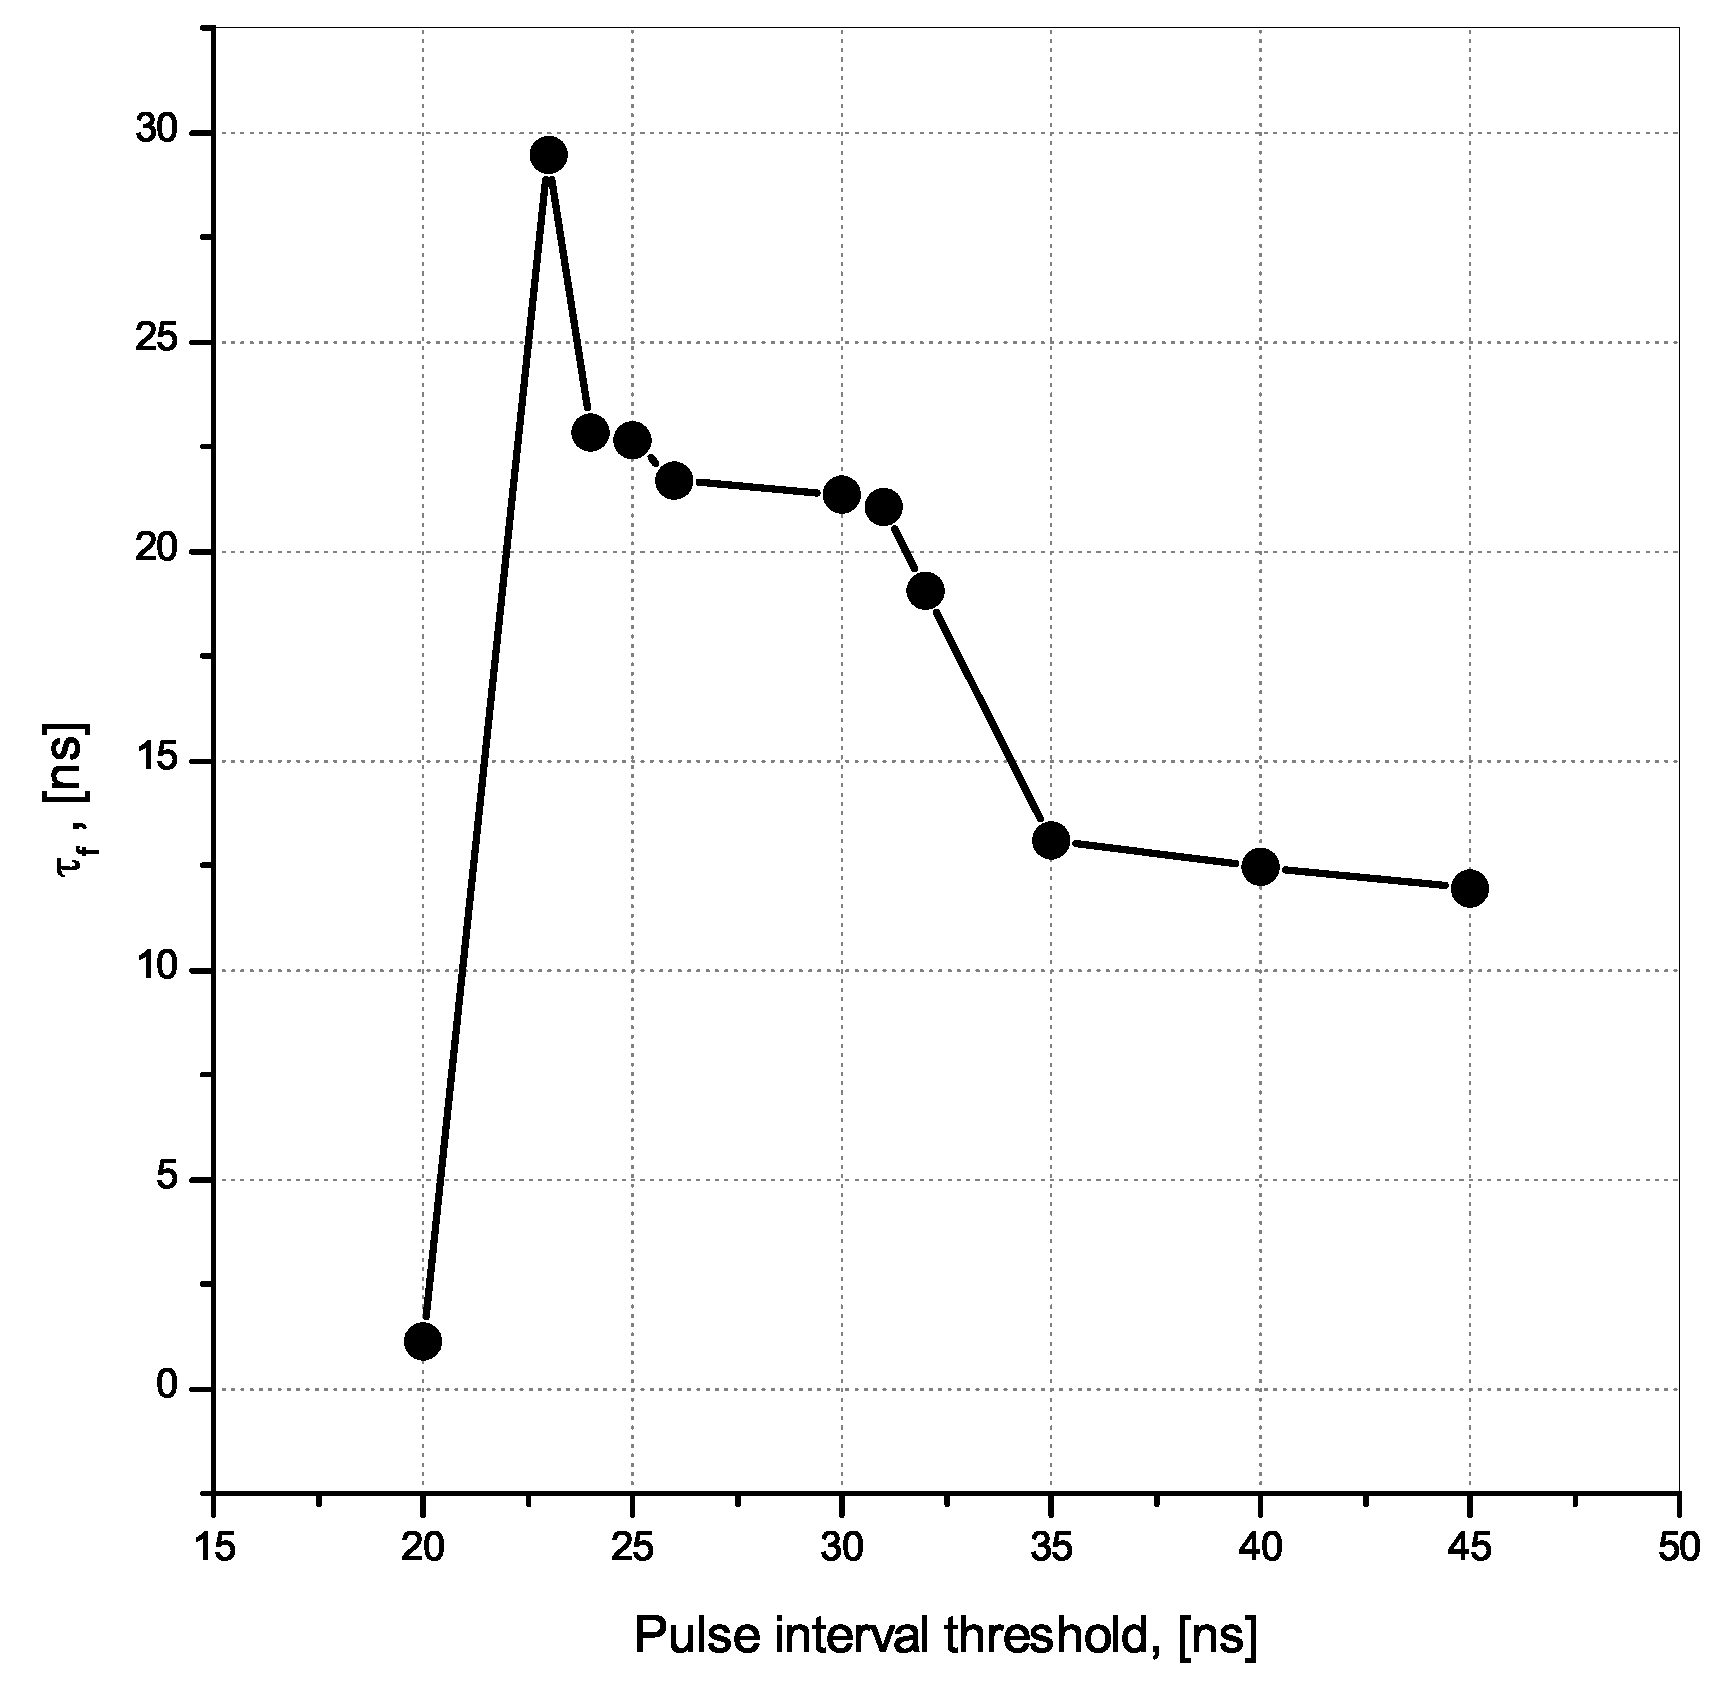
\includegraphics[width=0.47\textwidth]{Hamamatsu_S10362-11-100C_295K_1_OV_dt_spectrum_timecut_eng}
\\
\parbox[t]{0.47\textwidth}{\caption{The pulse interval spectrum approximated by Eq.(\ref{eq:dt_probability_fast_slow}).
Events with cross-talk are not taken into account.
The signal was obtained from Hamamatsu S10362-11-100C at 1V overvoltage and 295K temperature.}
\label{image:Hamamatsu_S10362-11-100C_295K_1_OV_dt_spectrum}}
\hfill
\parbox[t]{0.47\textwidth}{\caption{The dependence of the after-pulse fast component from the pulse interval threshold.
The signal was obtained from Hamamatsu S10362-11-100C at 1V overvoltage and 295K temperature.}
\label{image:Hamamatsu_S10362-11-100C 295K_1_OV_dt_spectrum_timecut}}
\end{figure}

\section{Results}
\subsection{Dark noise}
As the result of the approximation of the pulse interval spectrum the dependence of dark noise rate on a temperature and an overvoltage were obtained (Fig.\ref{image:Hamamatsu_S10362-11-100C_dc_vs_T}, \ref{image:Hamamatsu_S10362-11-100C_dc_vs_V}, \ref{image:Hamamatsu_S13360-3050CS_dc_vs_V_rus}, \ref{image:KETEK_PM1125NS_SB0_dc_vs_V_rus}).
The dependence of dark noise rate on a temperature is expressed by the following formula \cite{Characterization of SiPM: temperature dependencies}:
\begin{eqnarray}\label{eq:Hz_vs_temperature}
\nu(\Delta V = const, T) = A \cdot T^{3/2} \cdot \exp\left[ - \frac{E_g}{2 k_B \cdot T} \right],
\end{eqnarray}
where $A$ is a constant, depending on a voltage, the material and technological parameters, T is an absolute temperature, $E_g$ is a bandgap, $k_B$ is the Boltzmann constant.
The dependence of dark noise rate on an overvoltage is expressed by the linear law:
\begin{eqnarray}\label{eq:Hz_vs_overvoltage}
\nu(\Delta V, T = const) = k \cdot \Delta V
\end{eqnarray}


\begin{figure}[h]
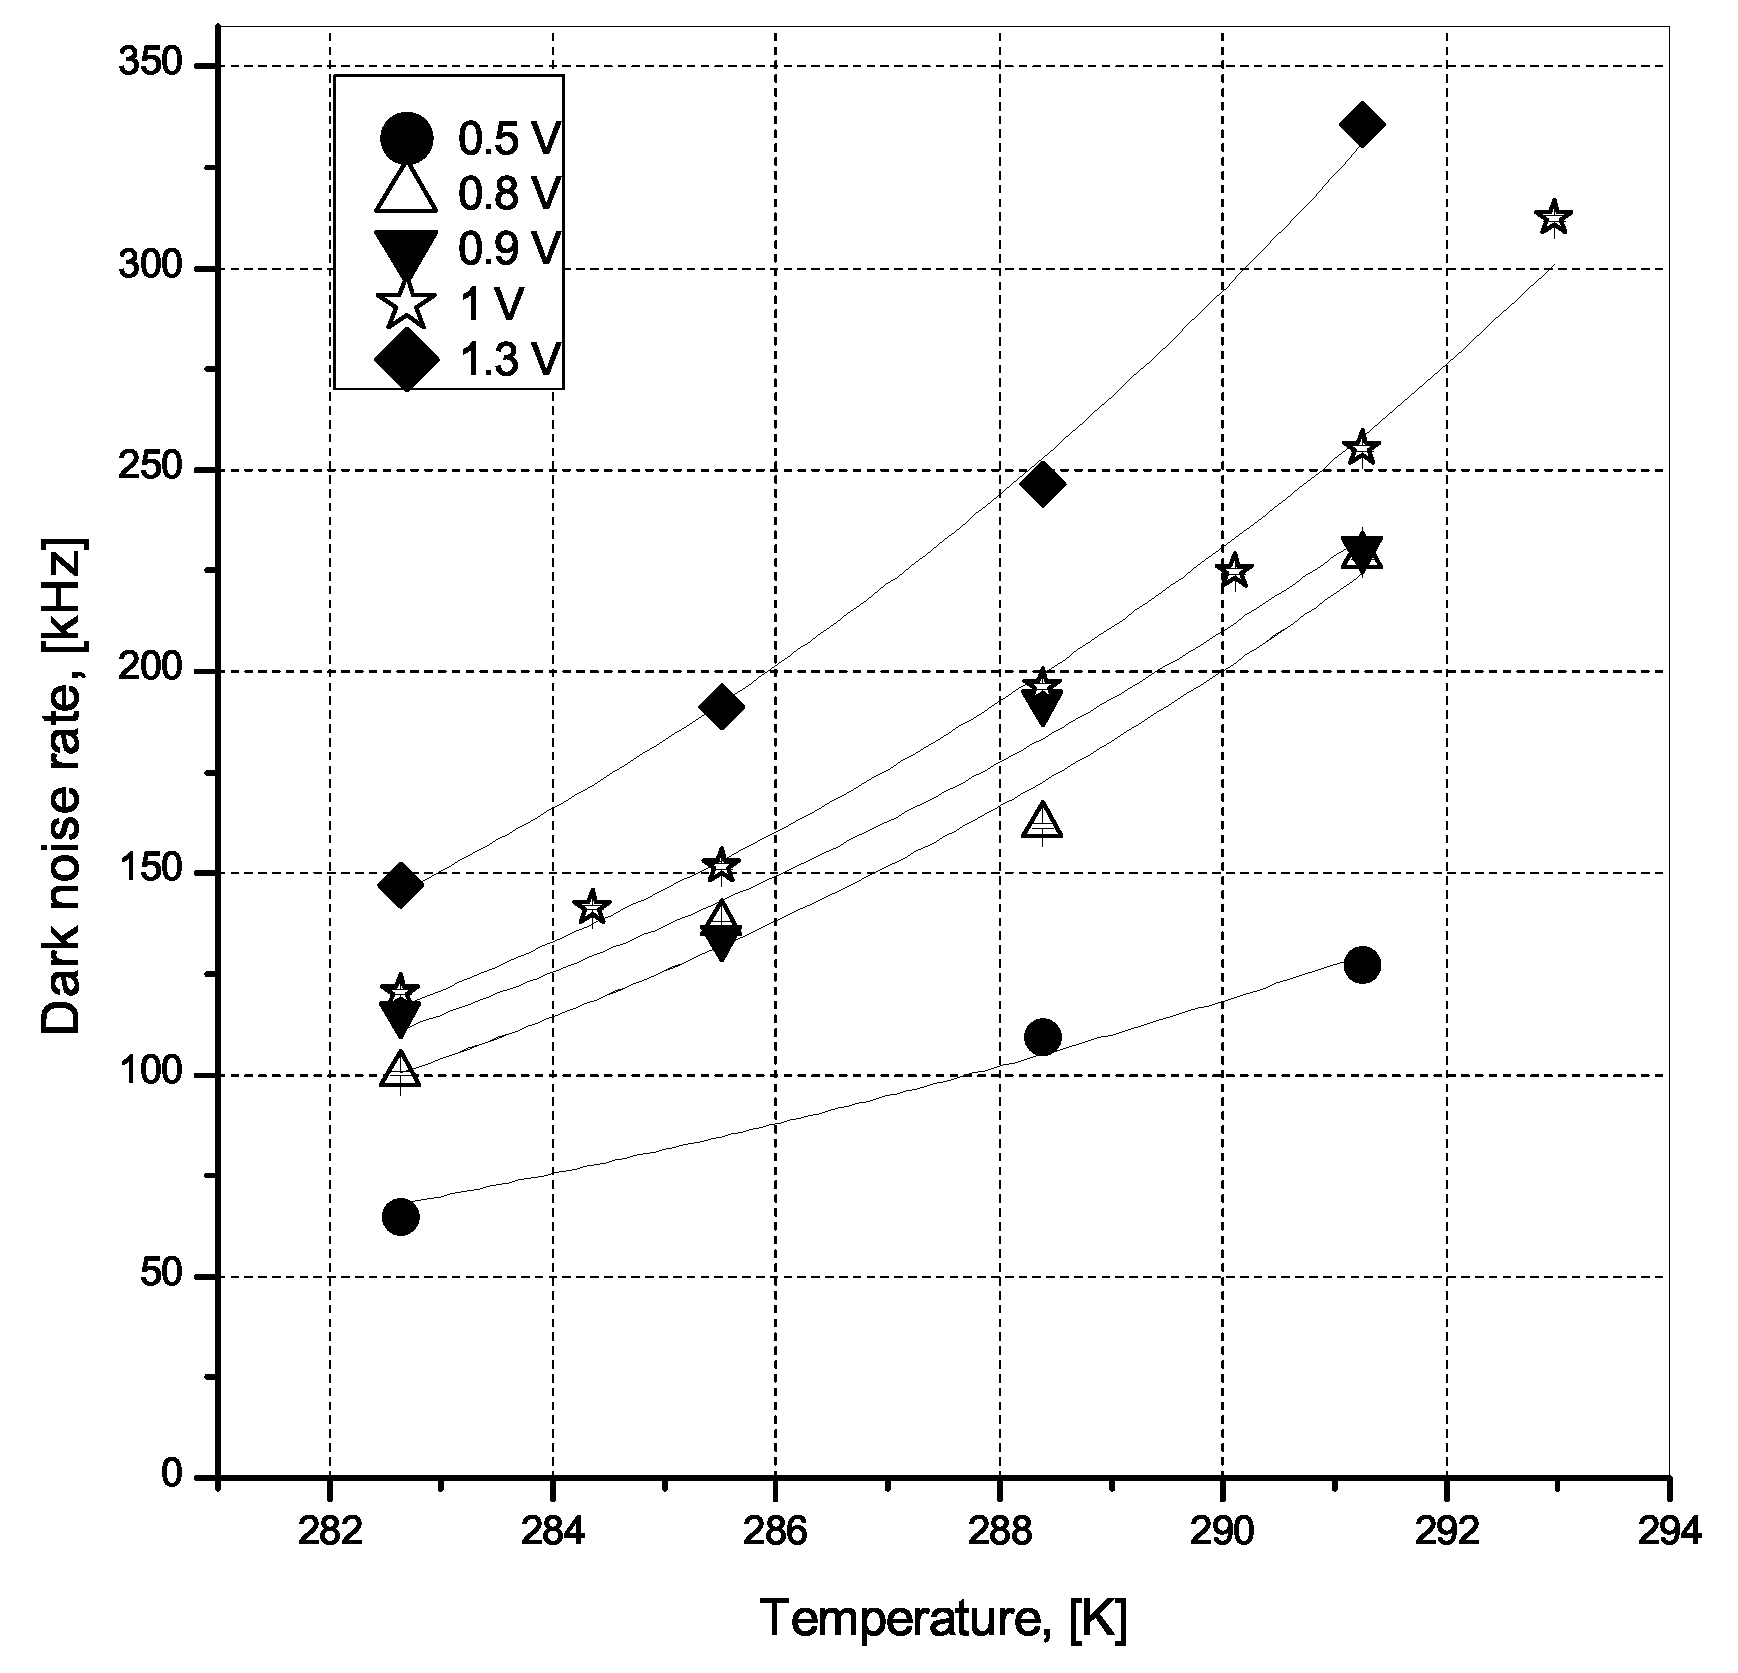
\includegraphics[width=0.47\textwidth]{Hamamatsu_S10362-11-100C_dc_vs_T_eng}
\hfill
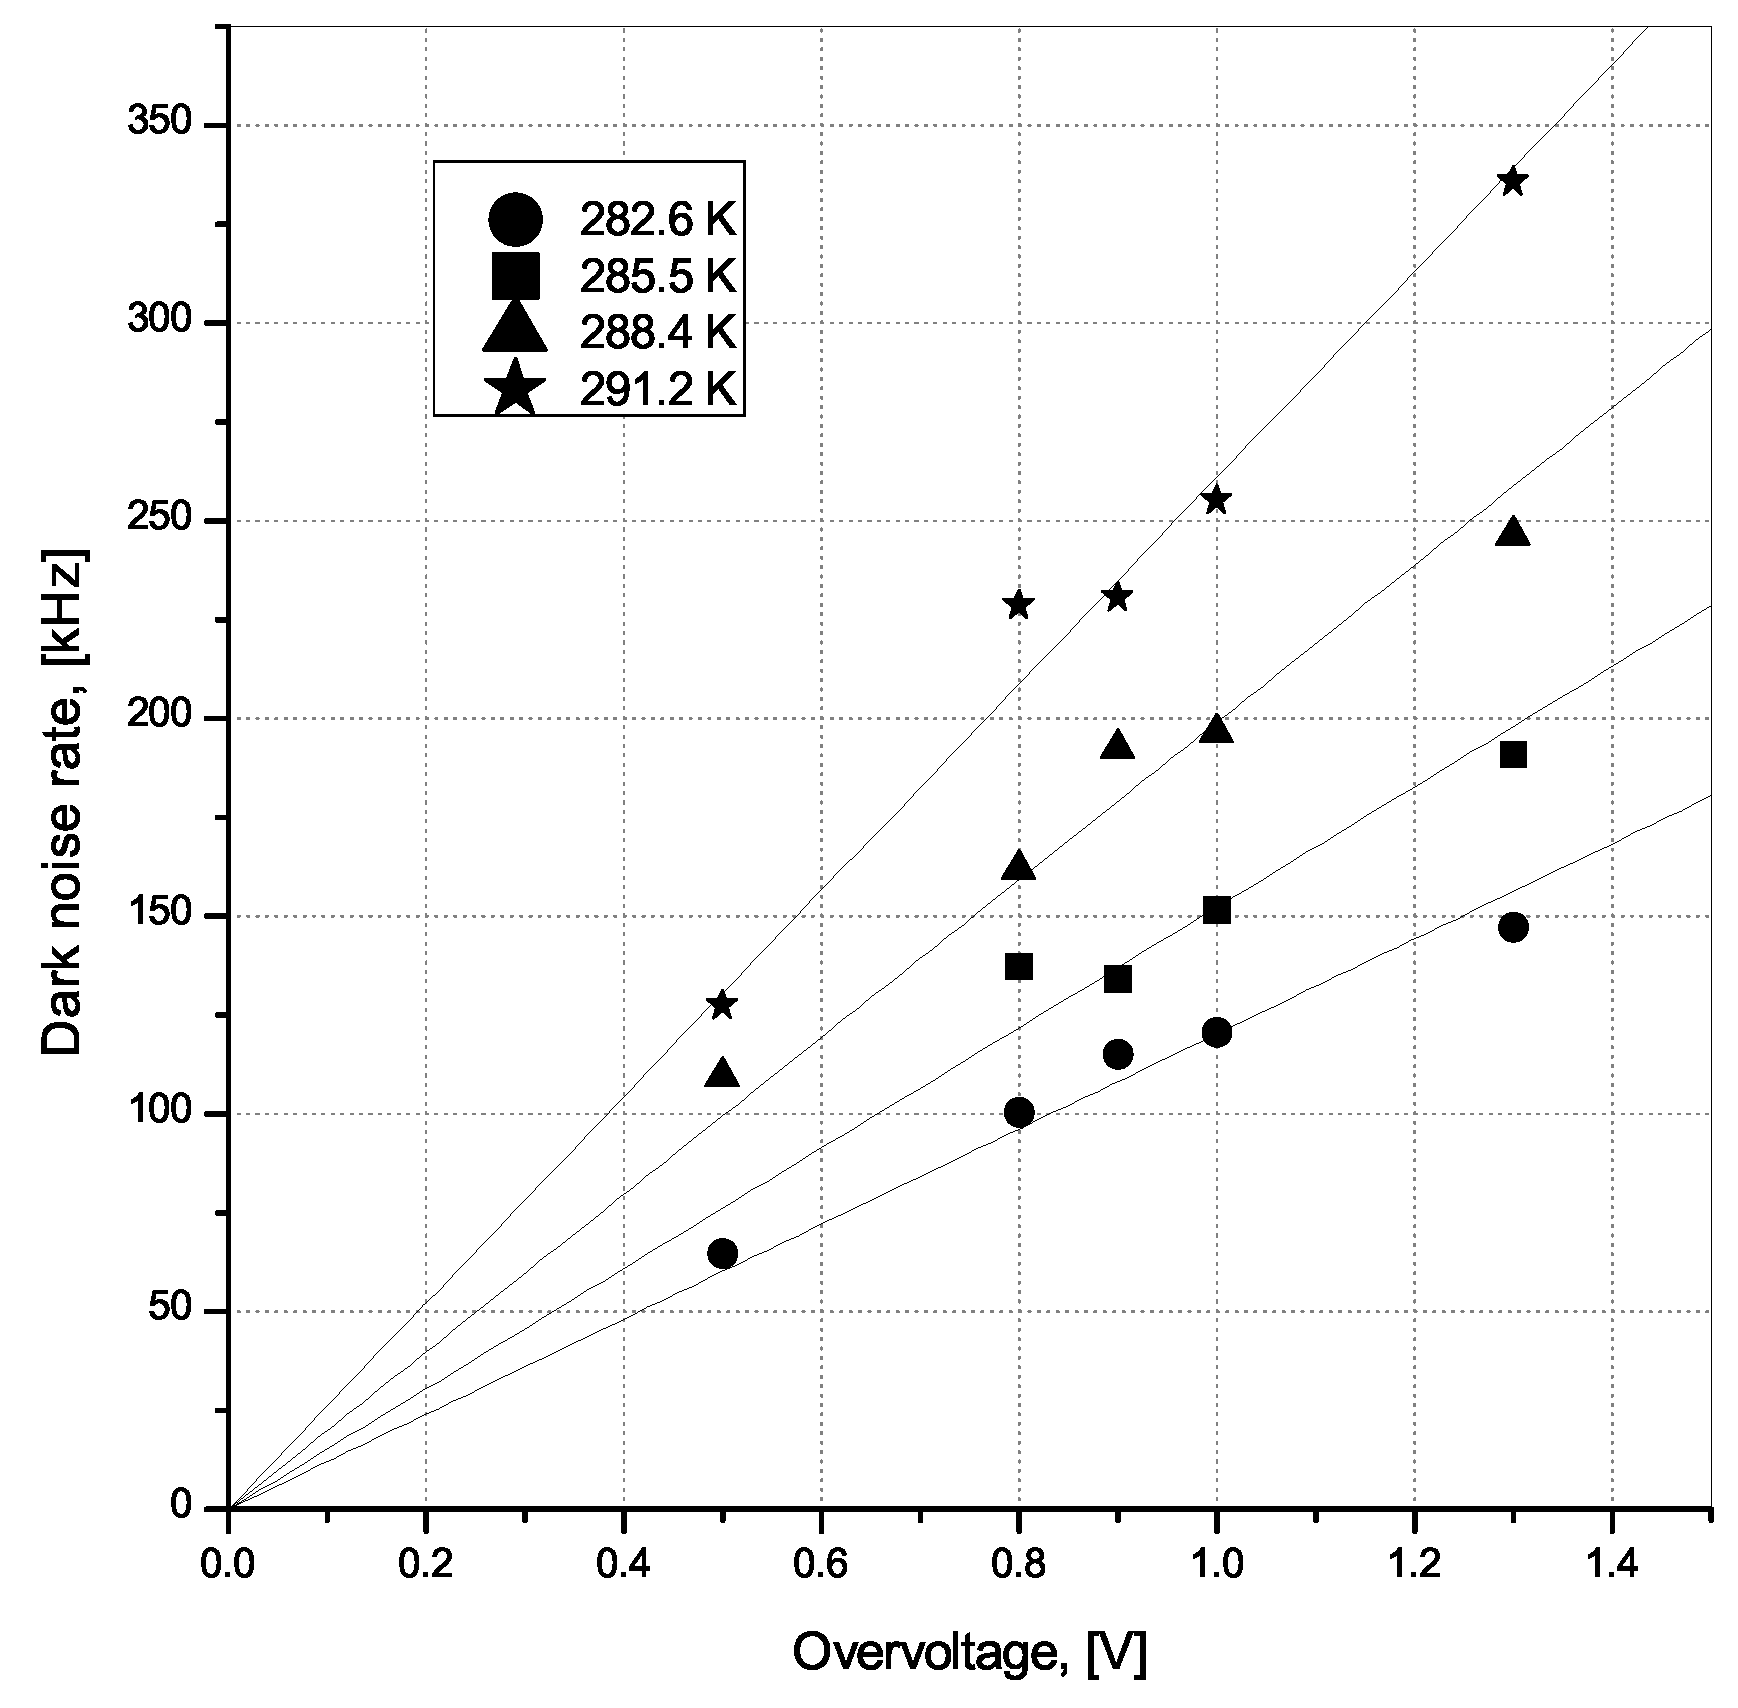
\includegraphics[width=0.47\textwidth]{Hamamatsu_S10362-11-100C_dc_vs_V_eng}
\\
\parbox[t]{0.47\textwidth}{\caption{The dependence of dark noise rate on a temperature at a fixed overvoltage for
Hamamatsu S10362-11-100C. The data were approximated by Eq.(\ref{eq:Hz_vs_temperature}).}
\label{image:Hamamatsu_S10362-11-100C_dc_vs_T}}
\hfill
\parbox[t]{0.47\textwidth}{\caption{The dependence of dark noise rate on a overvoltage at a fixed temperature for
Hamamatsu S10362-11-100C. The data were approximated by Eq.(\ref{eq:Hz_vs_overvoltage}).}
\label{image:Hamamatsu_S10362-11-100C_dc_vs_V}}
\end{figure}

\begin{figure}[h]
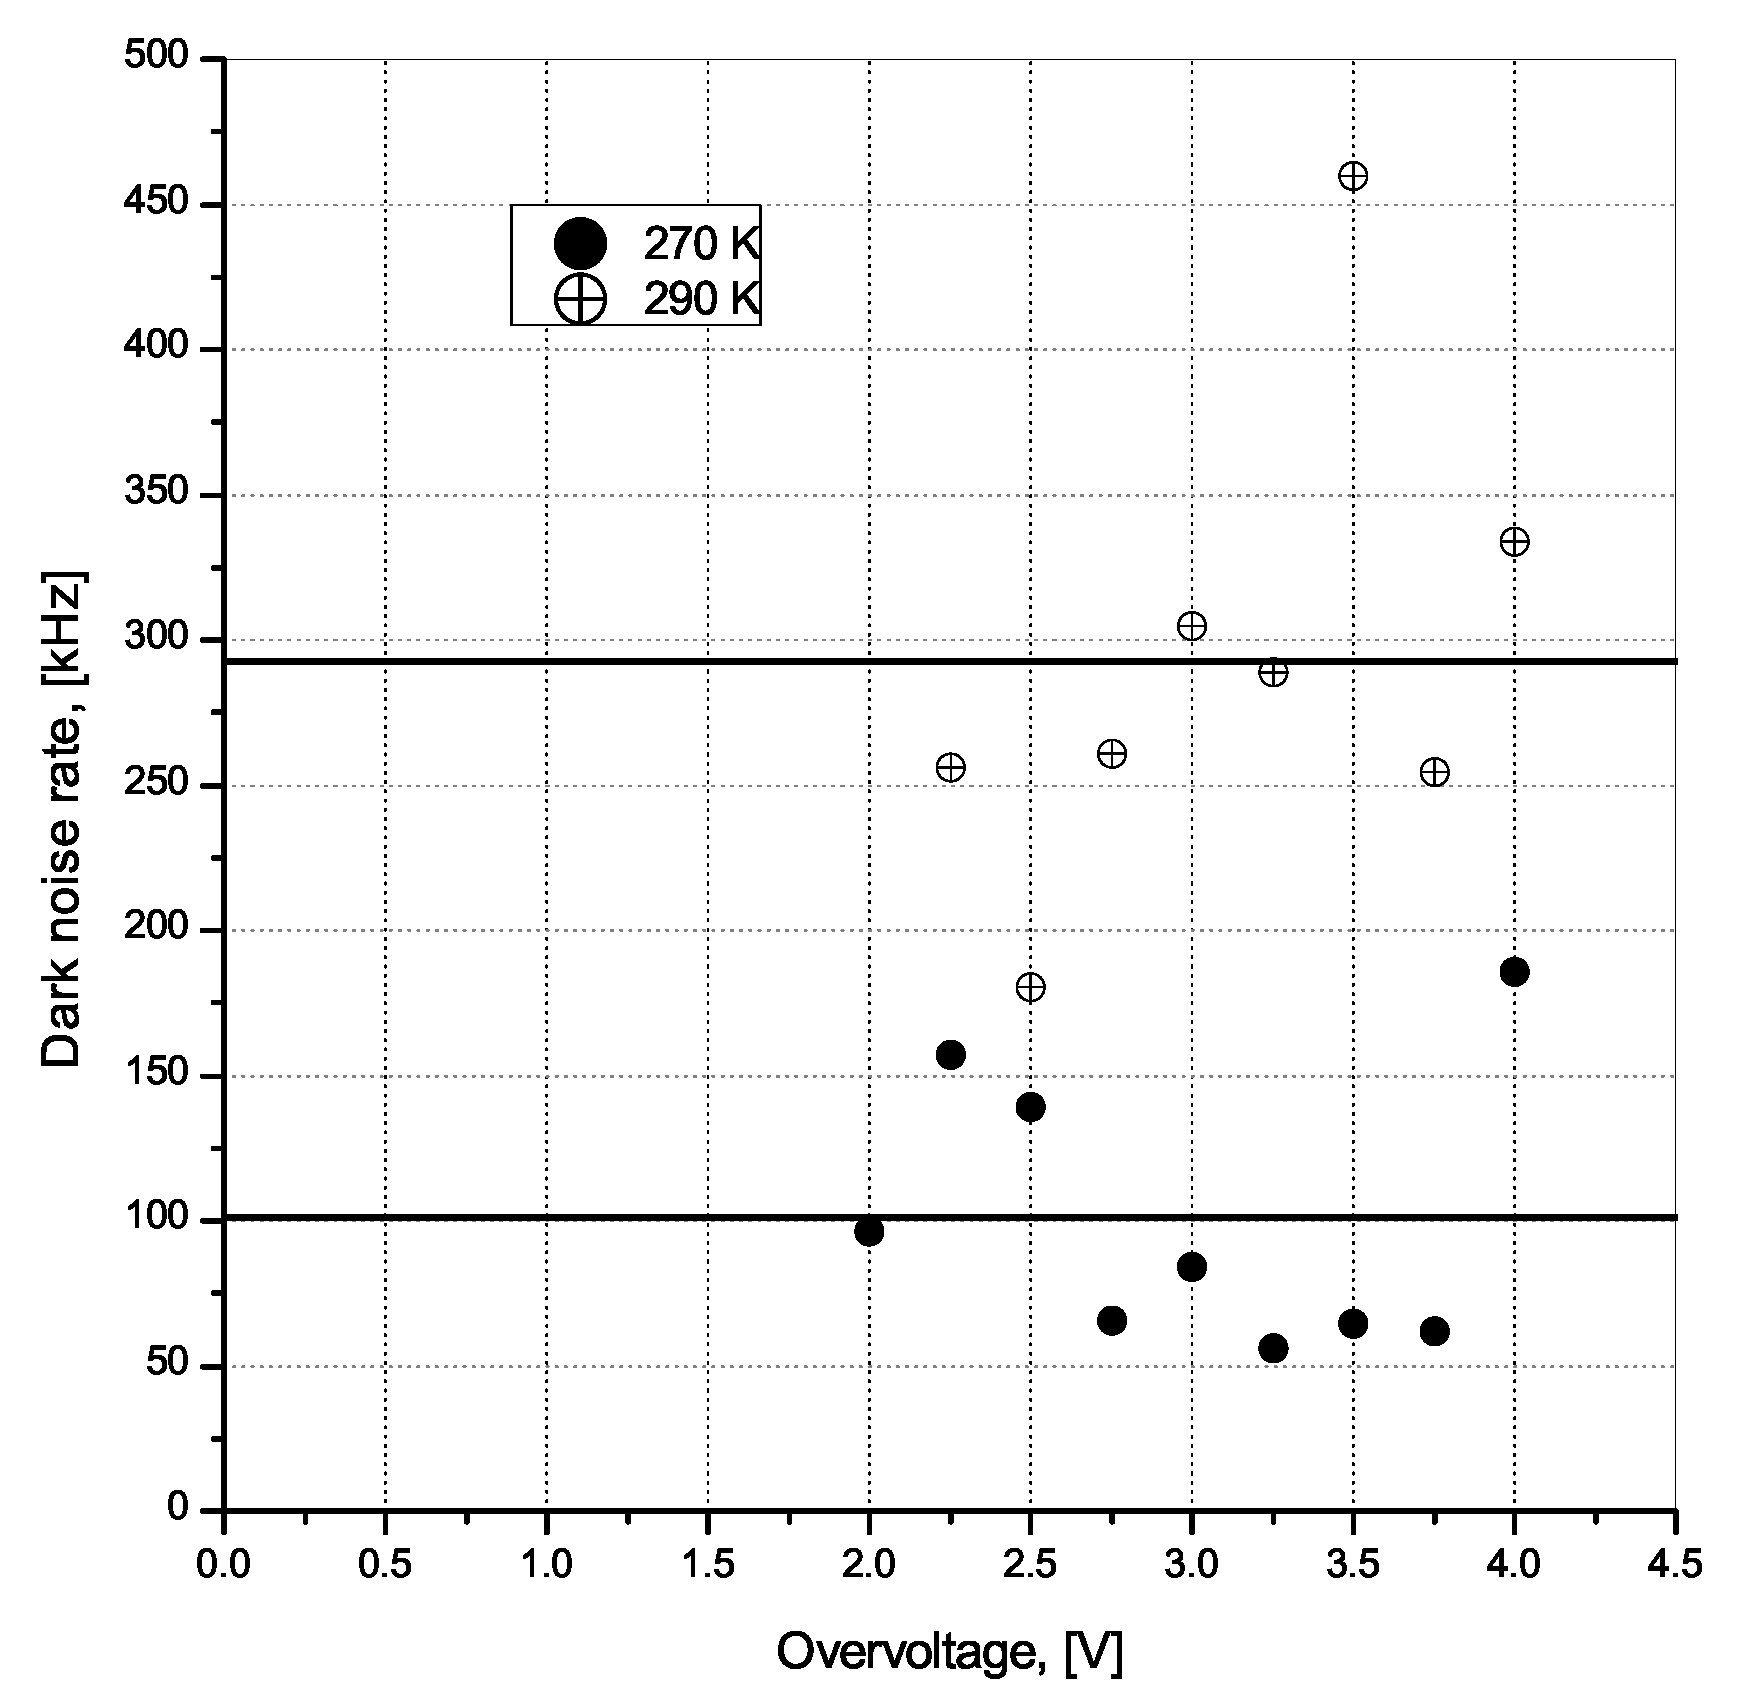
\includegraphics[width=0.47\textwidth]{Hamamatsu_S13360-3050CS_dc_vs_V_eng}
\hfill
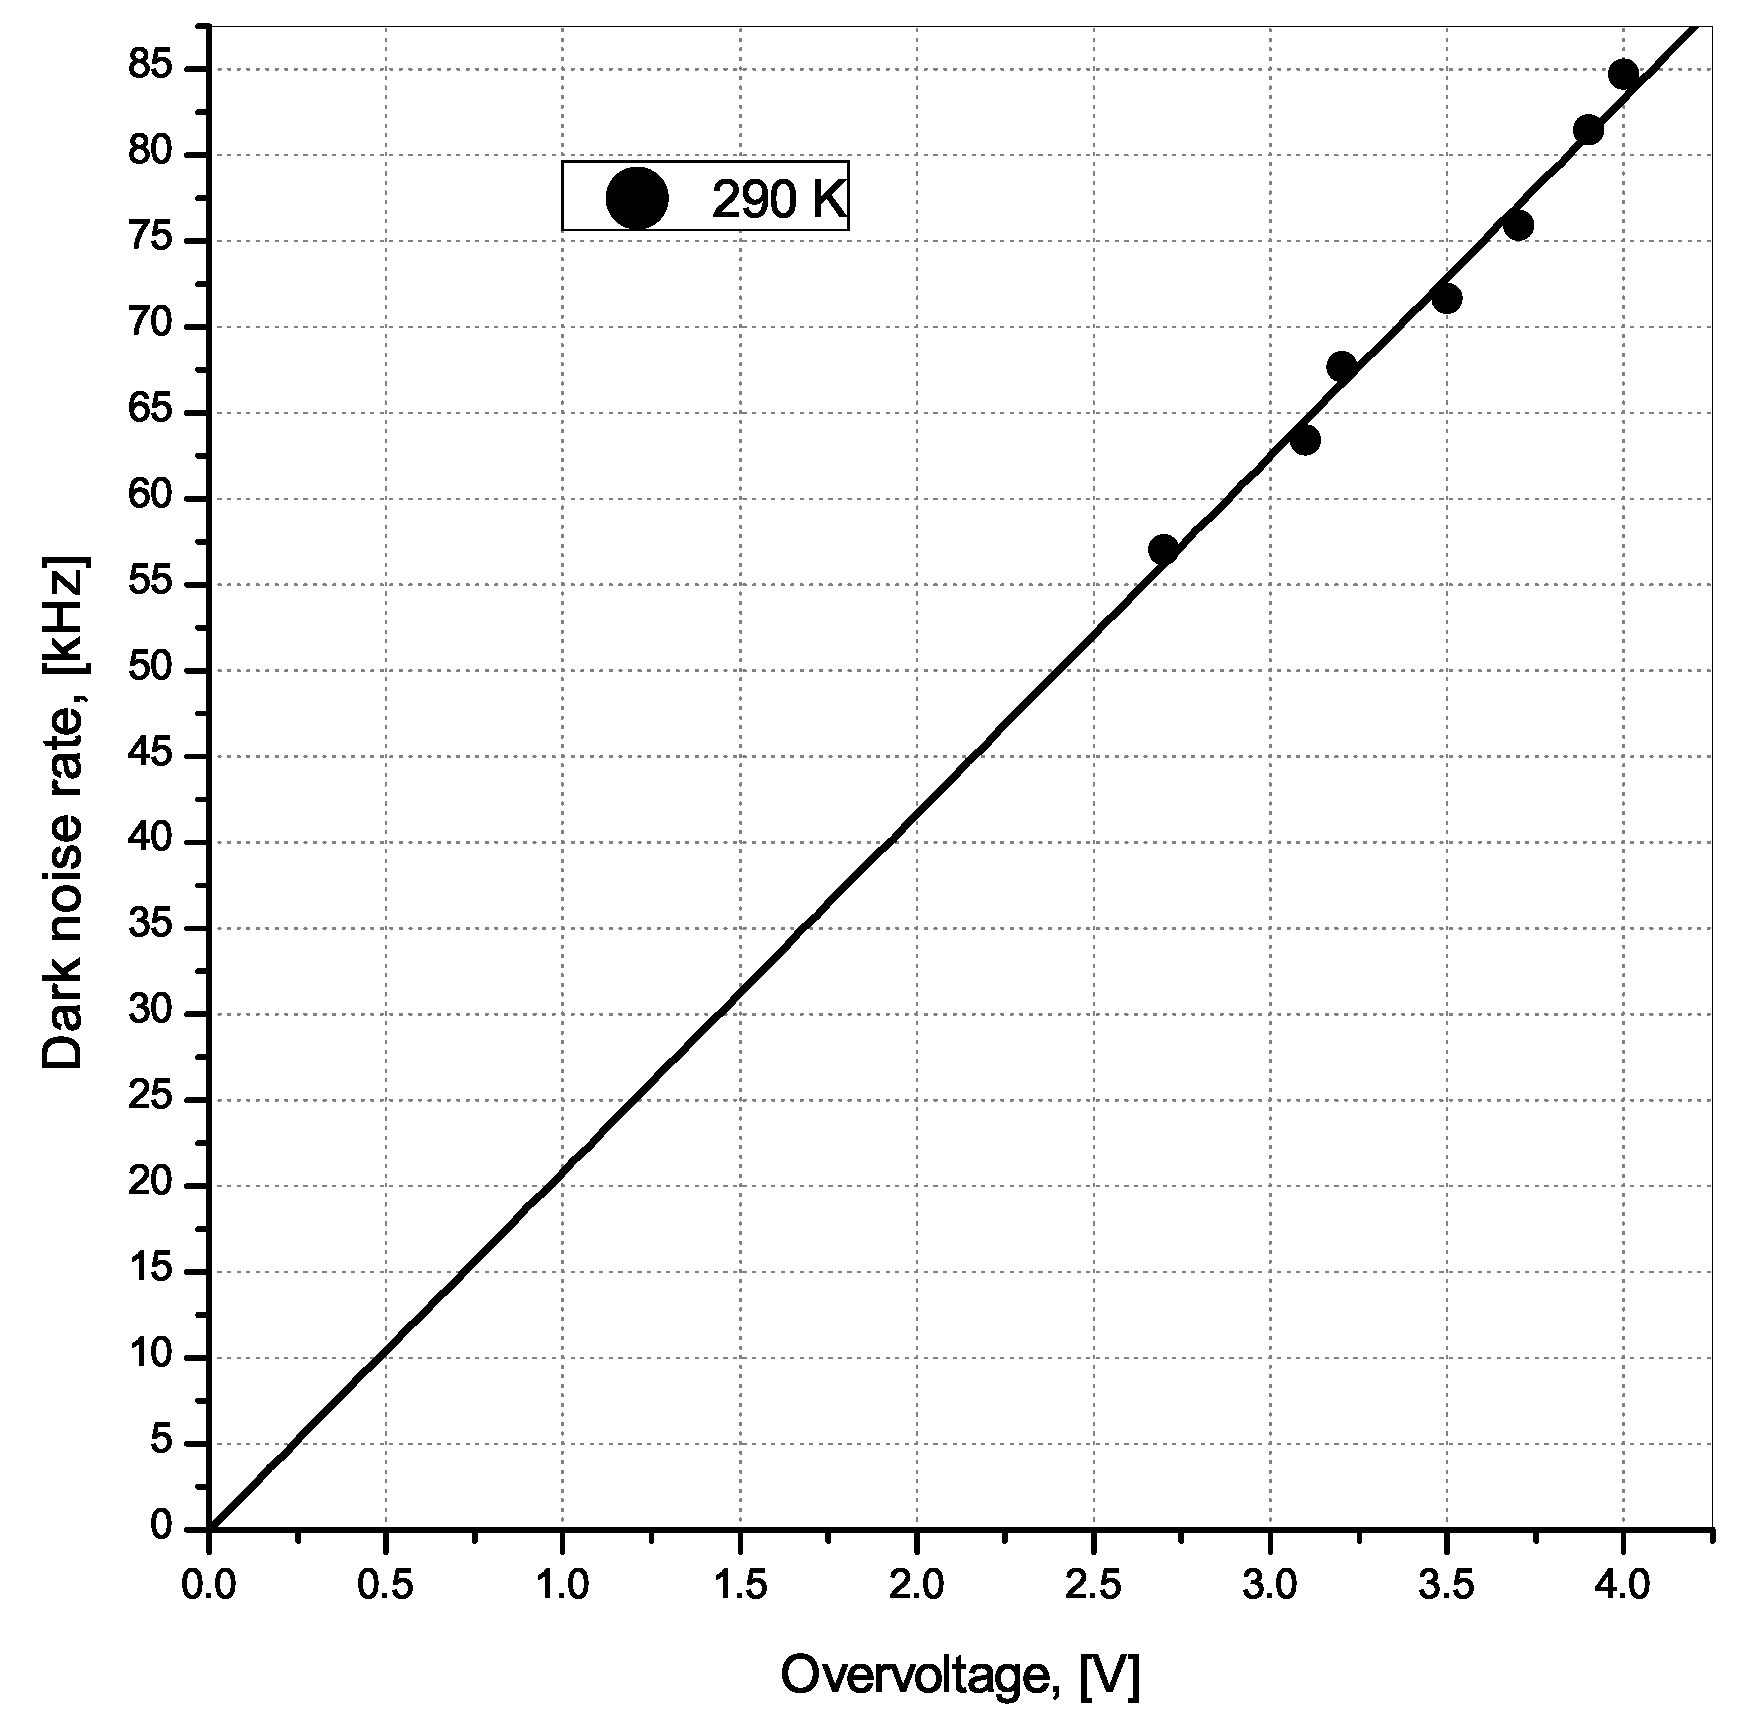
\includegraphics[width=0.47\textwidth]{KETEK_PM1125NS_SB0_dc_vs_V_eng}
\\
\parbox[t]{0.47\textwidth}{\caption{The dependence of dark noise rate on a overvoltage at a fixed temperature for Hamamatsu S13360-3050CS.
Lines are approximation of the data by constant for different temperatures.}
\label{image:Hamamatsu_S13360-3050CS_dc_vs_V_rus}}
\hfill
\parbox[t]{0.47\textwidth}{\caption{The dependence of dark noise rate on a overvoltage at a fixed temperature for KETEK PM1125NS-SB0.
The line is approximation of the data by linear function.}
\label{image:KETEK_PM1125NS_SB0_dc_vs_V_rus}}
\end{figure}


However we were failed to collect enough statistics for data approximation in this manner for Hamamatsu S13360-3050CS because of its low noise level.
For the same reason, only one point at the maximum noise level was obtained for KETEK PM1125NS-SB0.


\subsection{Cross-talk}
The $A_{1}$ cluster (Fig.~\ref{image:Hamamatsu_S10362-11-100C_295K_1V_Chi2_amp 1}) consists of single-electron pulses.
The $B_{1}$ cluster consists of pulses caused by the simultaneous triggering of two cells.
The $C_{1}$ cluster consists of pulses caused by the simultaneous triggering of three cells.
The $A_{2}$ cluster (Fig.~\ref{image:Hamamatsu_S10362-11-100C_295K_1_OV_Chi2_amp1_amp2}) consists of pulses caused by triggering of one cell with the subsequent after-pulse or triggering two cells at different time points because of dark noise.
The $B_{2}$ cluster consists of pulses caused by the simultaneous triggering of two cells with the subsequent after-pulse of one of the cells or triggering of one cell with the subsequent after-pulse, causing cross-talk.

At the moment, we calculate the cross-talk probability as follows:
\begin{eqnarray}\label{eq:xtalk_general}
P_{X-talk} = ( N_{B_{1}} + N_{C_{1}} ) / (N_{A_{1}} + N_{B_{1}} + N_{C_{1}})
\end{eqnarray}
This is an approximate formula because one should take into account the fact that a small part of with cross-talk events is contained in $B_{2}$, $C_{2}$, $B_{3}$, $C_{3}$, etc. clusters.

The cross-talk probability should have the quadratic dependence of an overvoltage in the first approximation.
This is explained by the cross-talk probability $P_{x-talk}$ is proportional to the number of electrons in the avalanche $G$ and the triggering probability of cells by photon $\varepsilon_{Geiger}$.
$G$ and $\varepsilon_{Geiger}$ have a linear dependence on an overvoltage(for $\varepsilon_{Geiger}$ value the dependence differs
from linear at a high overvoltage \cite{Measurement of PDE of MPPC with different wavelengths of light}):
\begin{eqnarray}\label{eq:xtalk_prob_V2_reason}
P_{x-talk}(\Delta V) \propto  G(\Delta V) \cdot \varepsilon_{Geiger}(\Delta V)
\end{eqnarray}

Thus, the experimental data were approximated by the following formula:
\begin{eqnarray}\label{eq:xtalk_vs_T_V}
P_{x-talk}(\Delta V, T) = k_{x-talk} \cdot \Delta V^2
\end{eqnarray}

The results of processing are shown on Fig. \ref{image:Hamamatsu_S10362-11-100C_xtalk_vs_T}, \ref{image:Hamamatsu_S10362-11-100C_xtalk_vs_V}, \ref{image:Hamamatsu_S13360-3050CS_xtalk_vs_V_rus}, \ref{image:KETEK_PM1125NS_SB0_x-tlak_vs_V_rus}.

\begin{figure}[h]
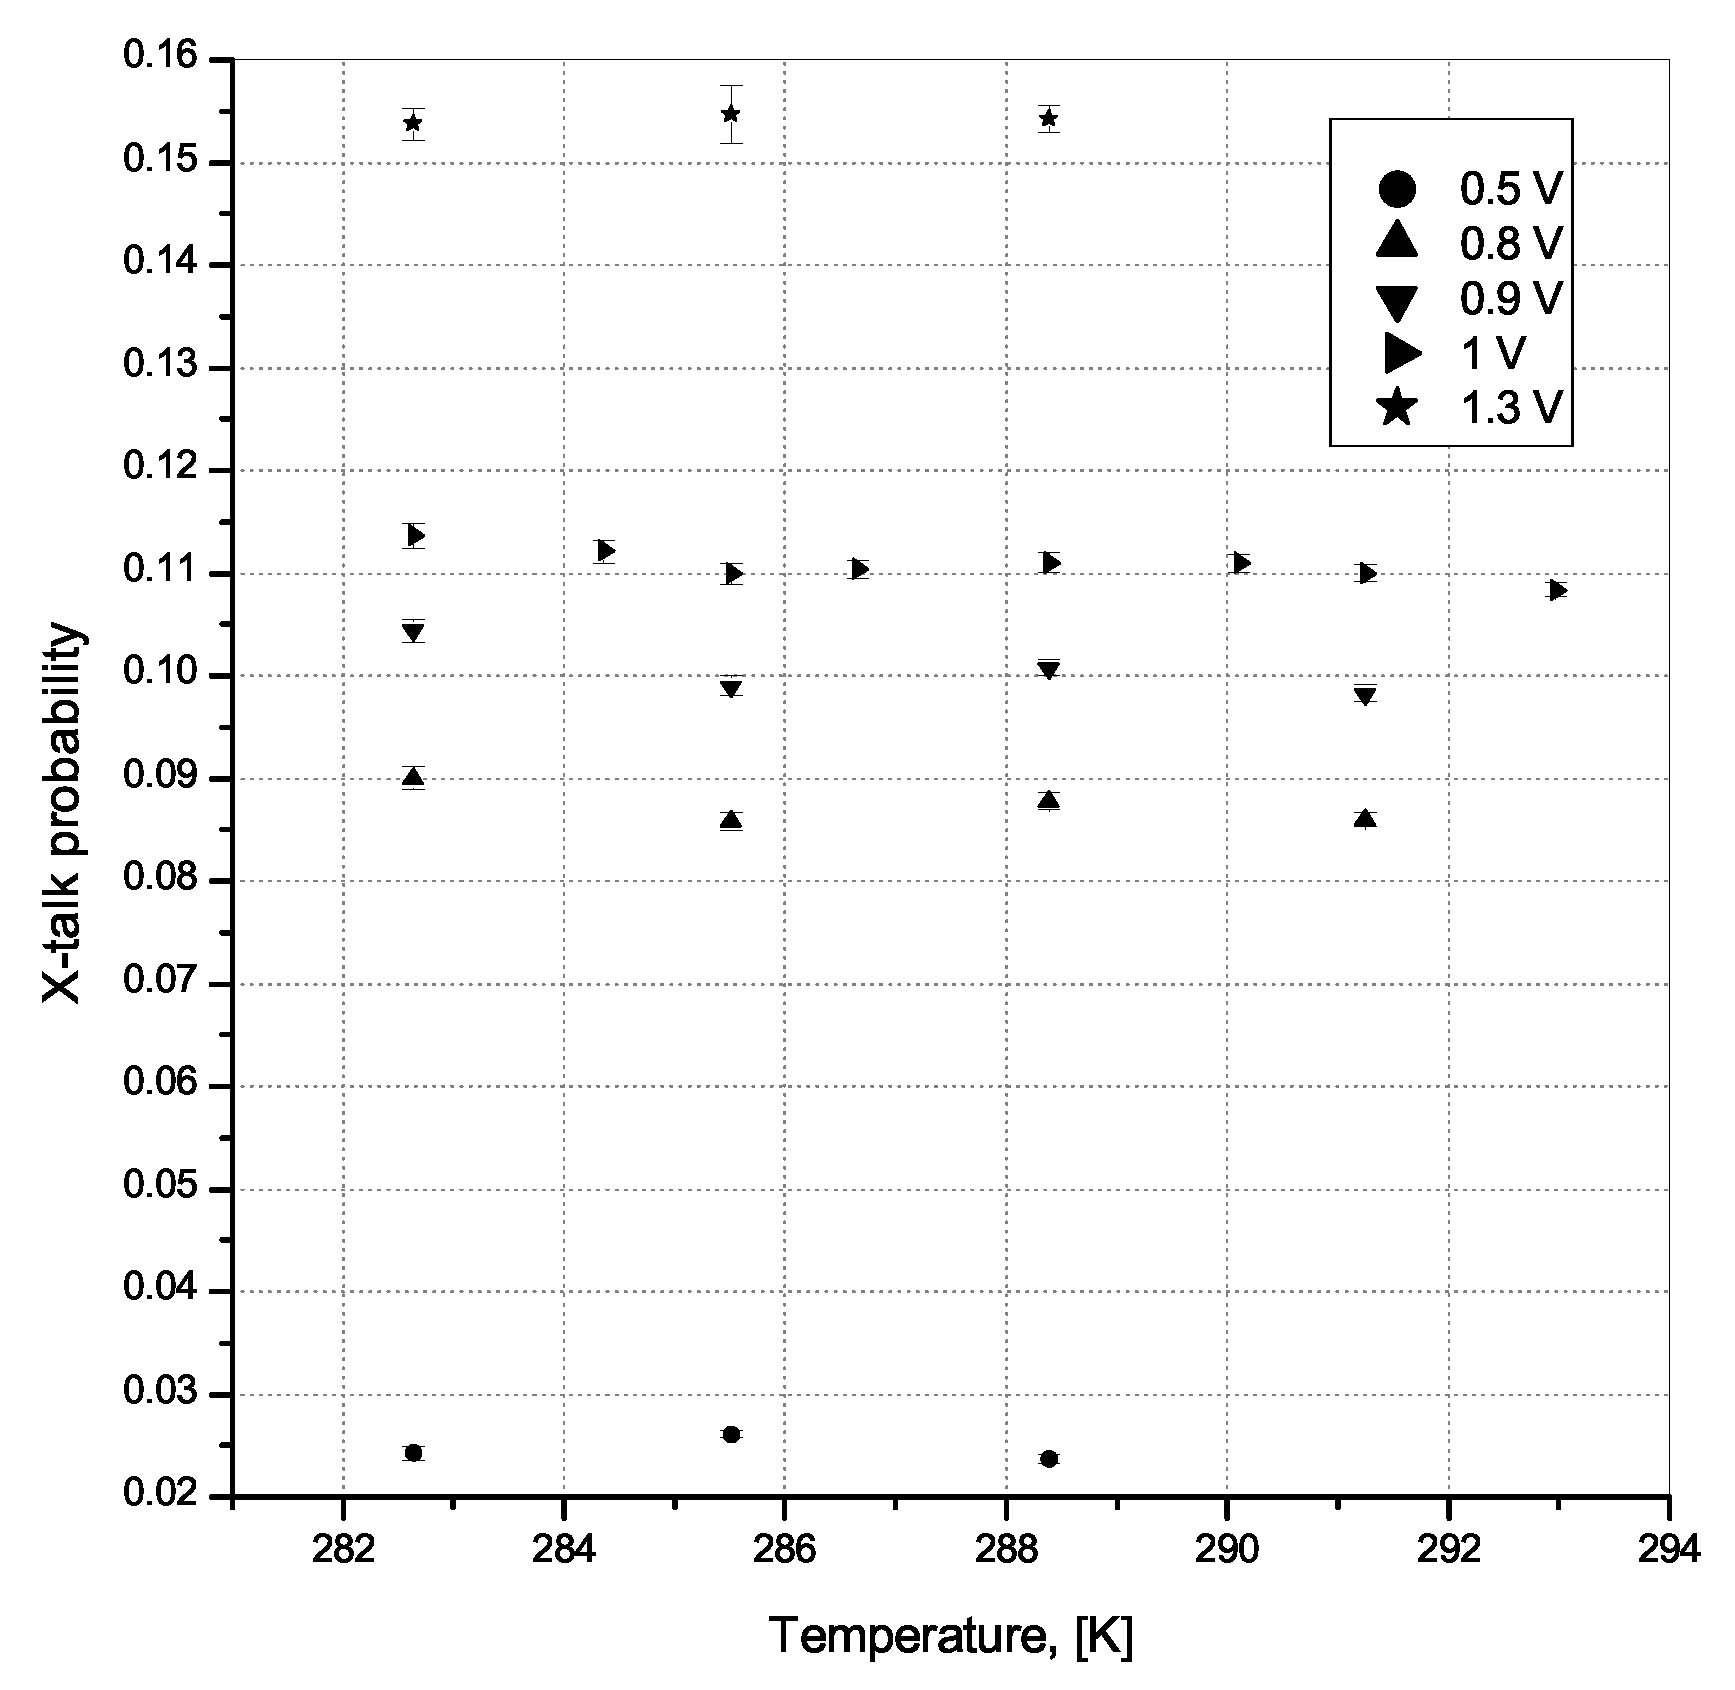
\includegraphics[width=0.47\textwidth]{Hamamatsu_S10362-11-100C_xtalk_vs_T_eng}
\hfill
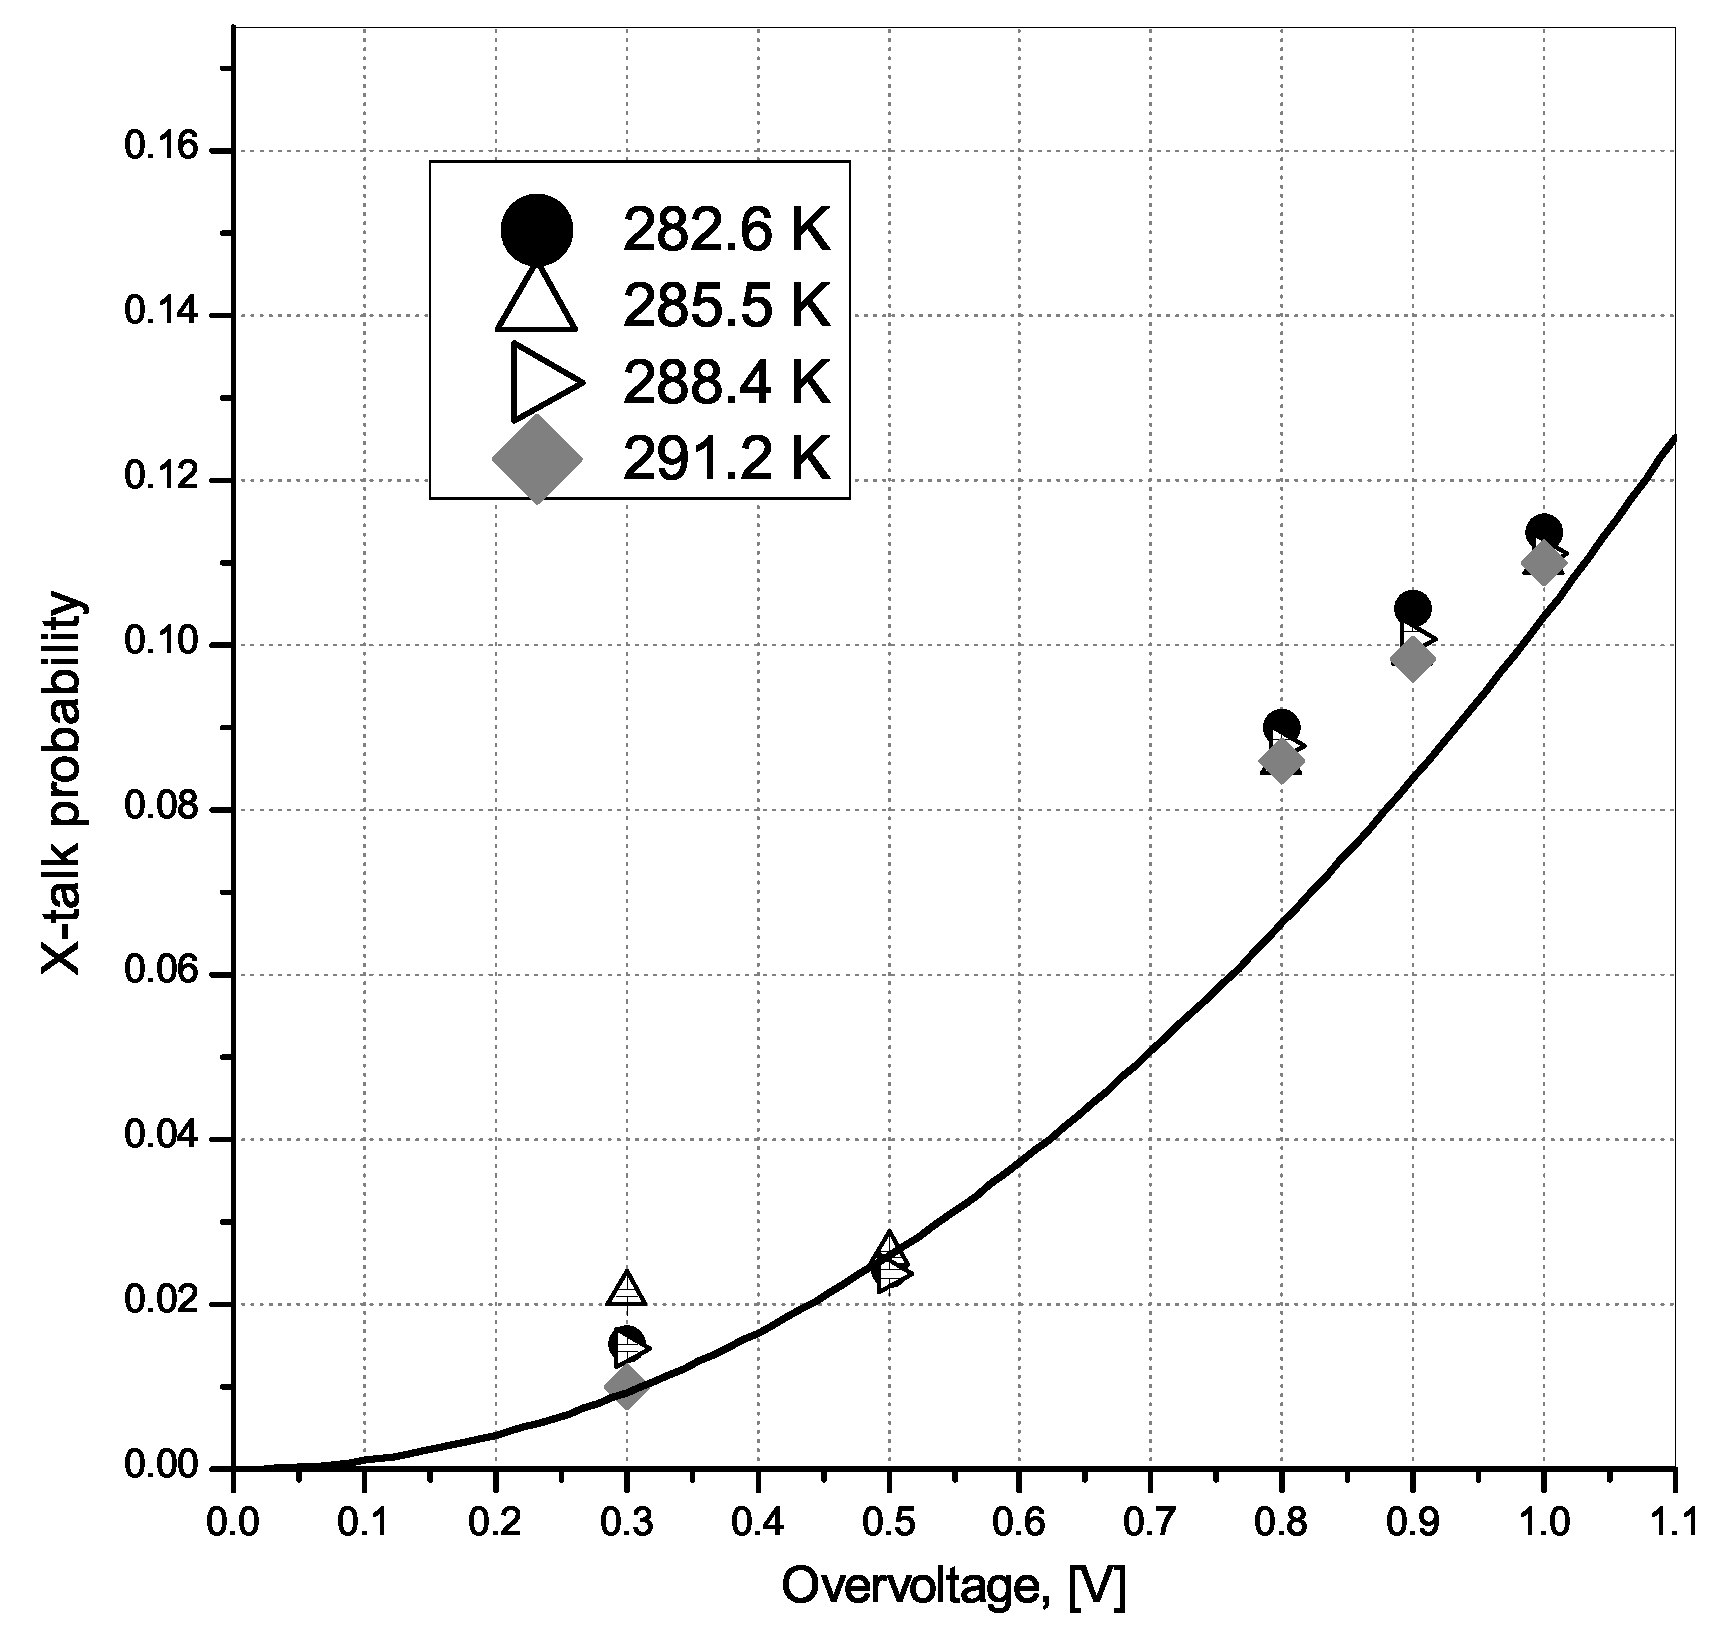
\includegraphics[width=0.47\textwidth]{Hamamatsu_S10362-11-100C_xtalk_vs_V_eng}
\\
\parbox[t]{0.47\textwidth}{\caption{The dependence of the cross-talk probability on a temperature at a fixed overvoltage for Hamamatsu S10362-11-100C.}
\label{image:Hamamatsu_S10362-11-100C_xtalk_vs_T}}
\hfill
\parbox[t]{0.47\textwidth}{\caption{The dependence of the cross-talk probability on a overvoltage at a fixed temperature for
Hamamatsu S10362-11-100C. The data were approximated by a quadratic function.}
\label{image:Hamamatsu_S10362-11-100C_xtalk_vs_V}}
\end{figure}

\begin{figure}[h]
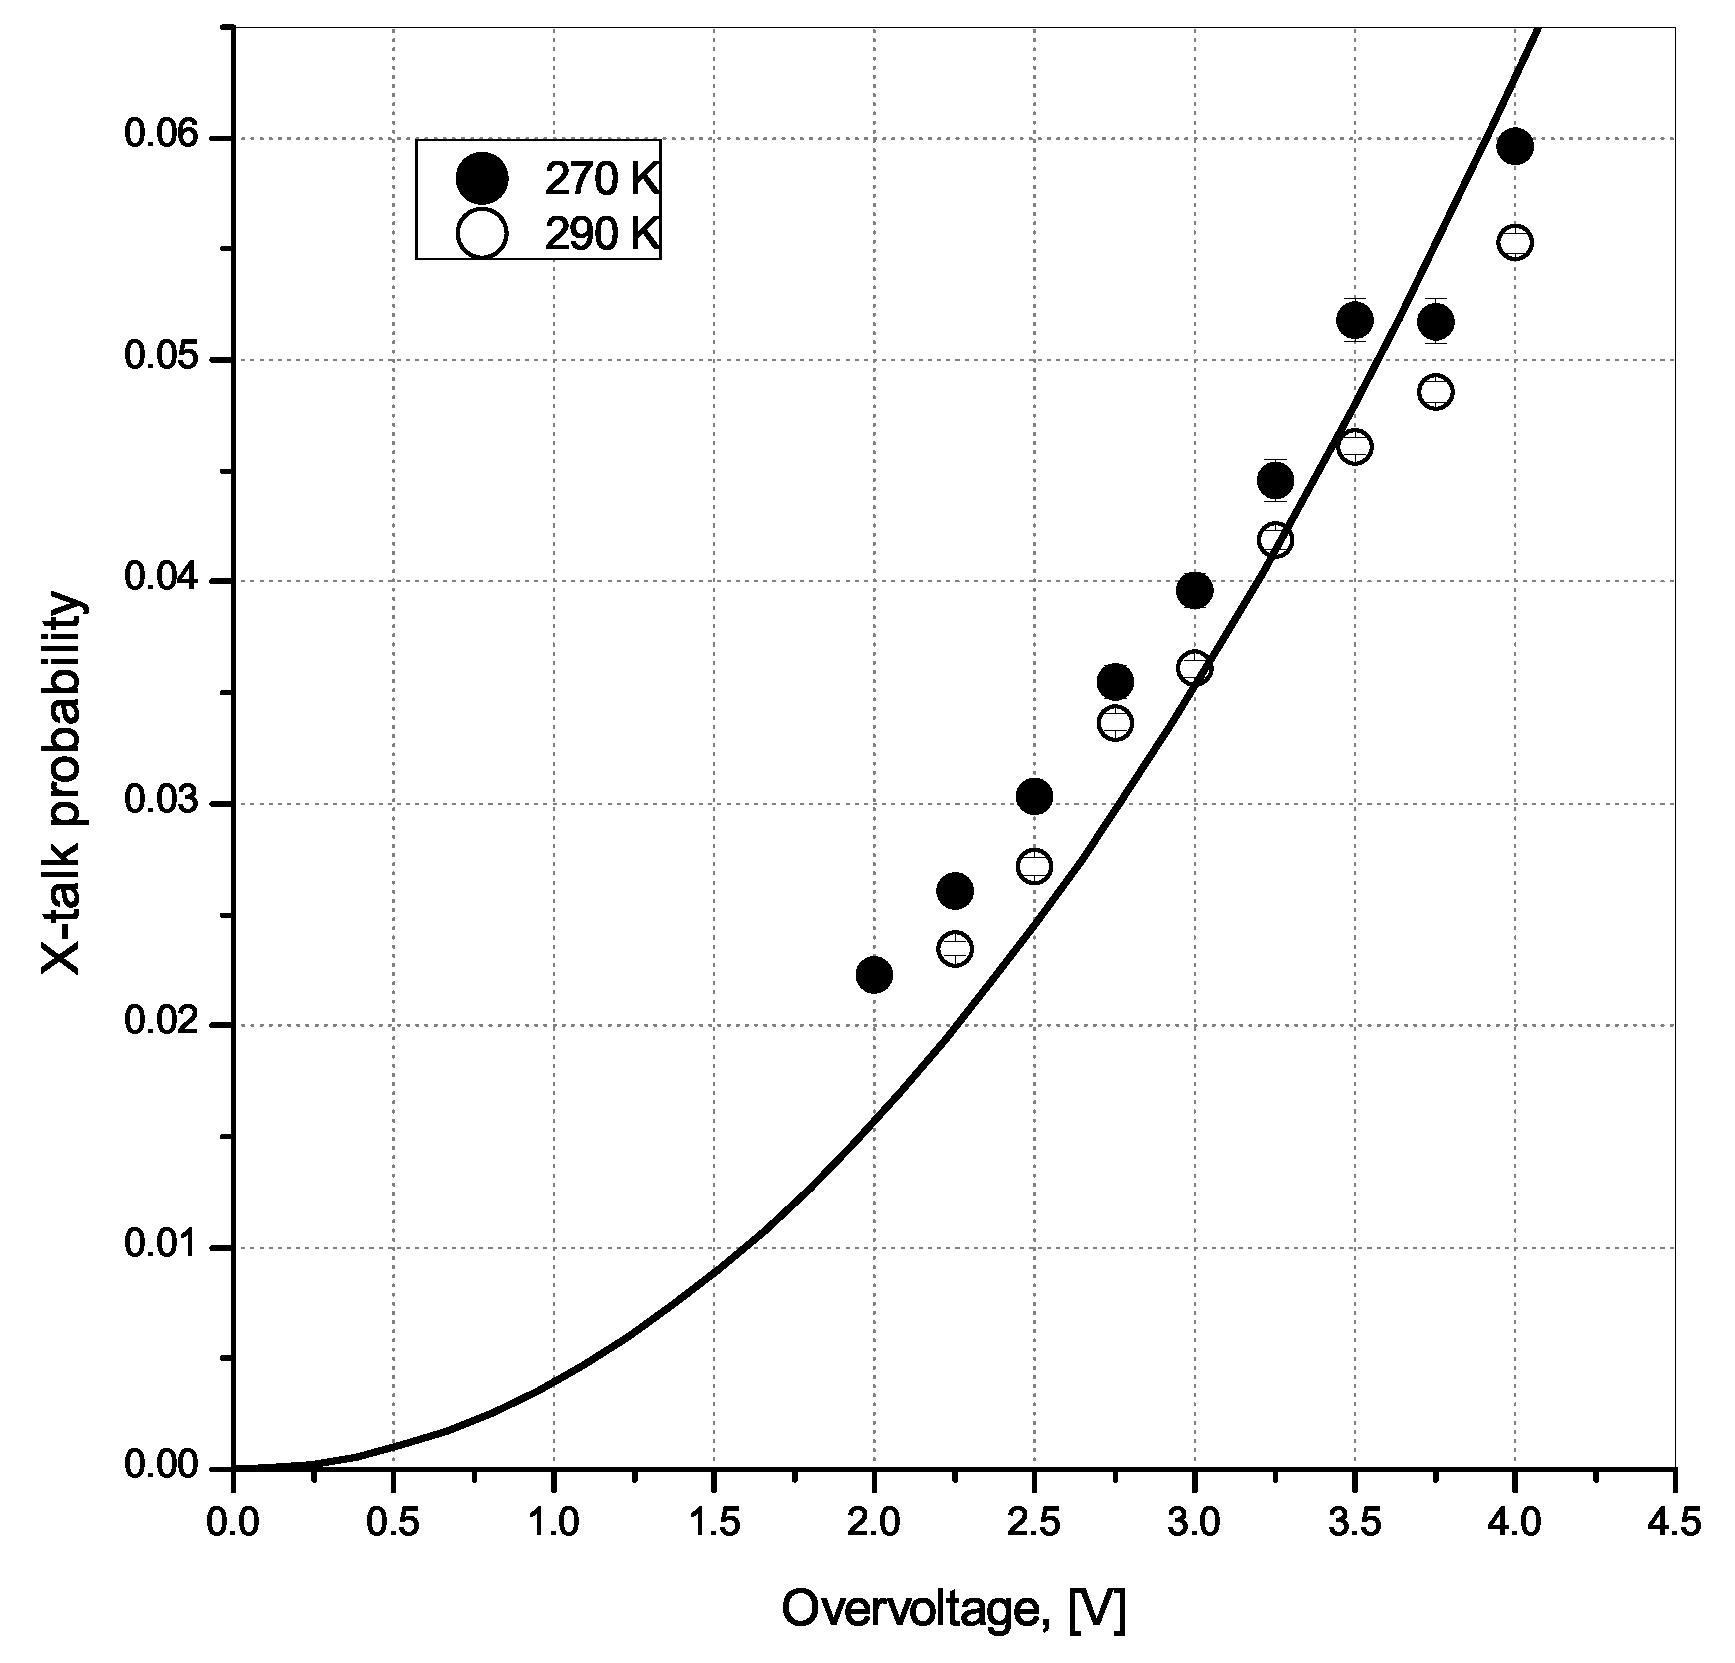
\includegraphics[width=0.47\textwidth]{Hamamatsu_S13360-3050CS_xtalk_vs_V_eng}
\hfill
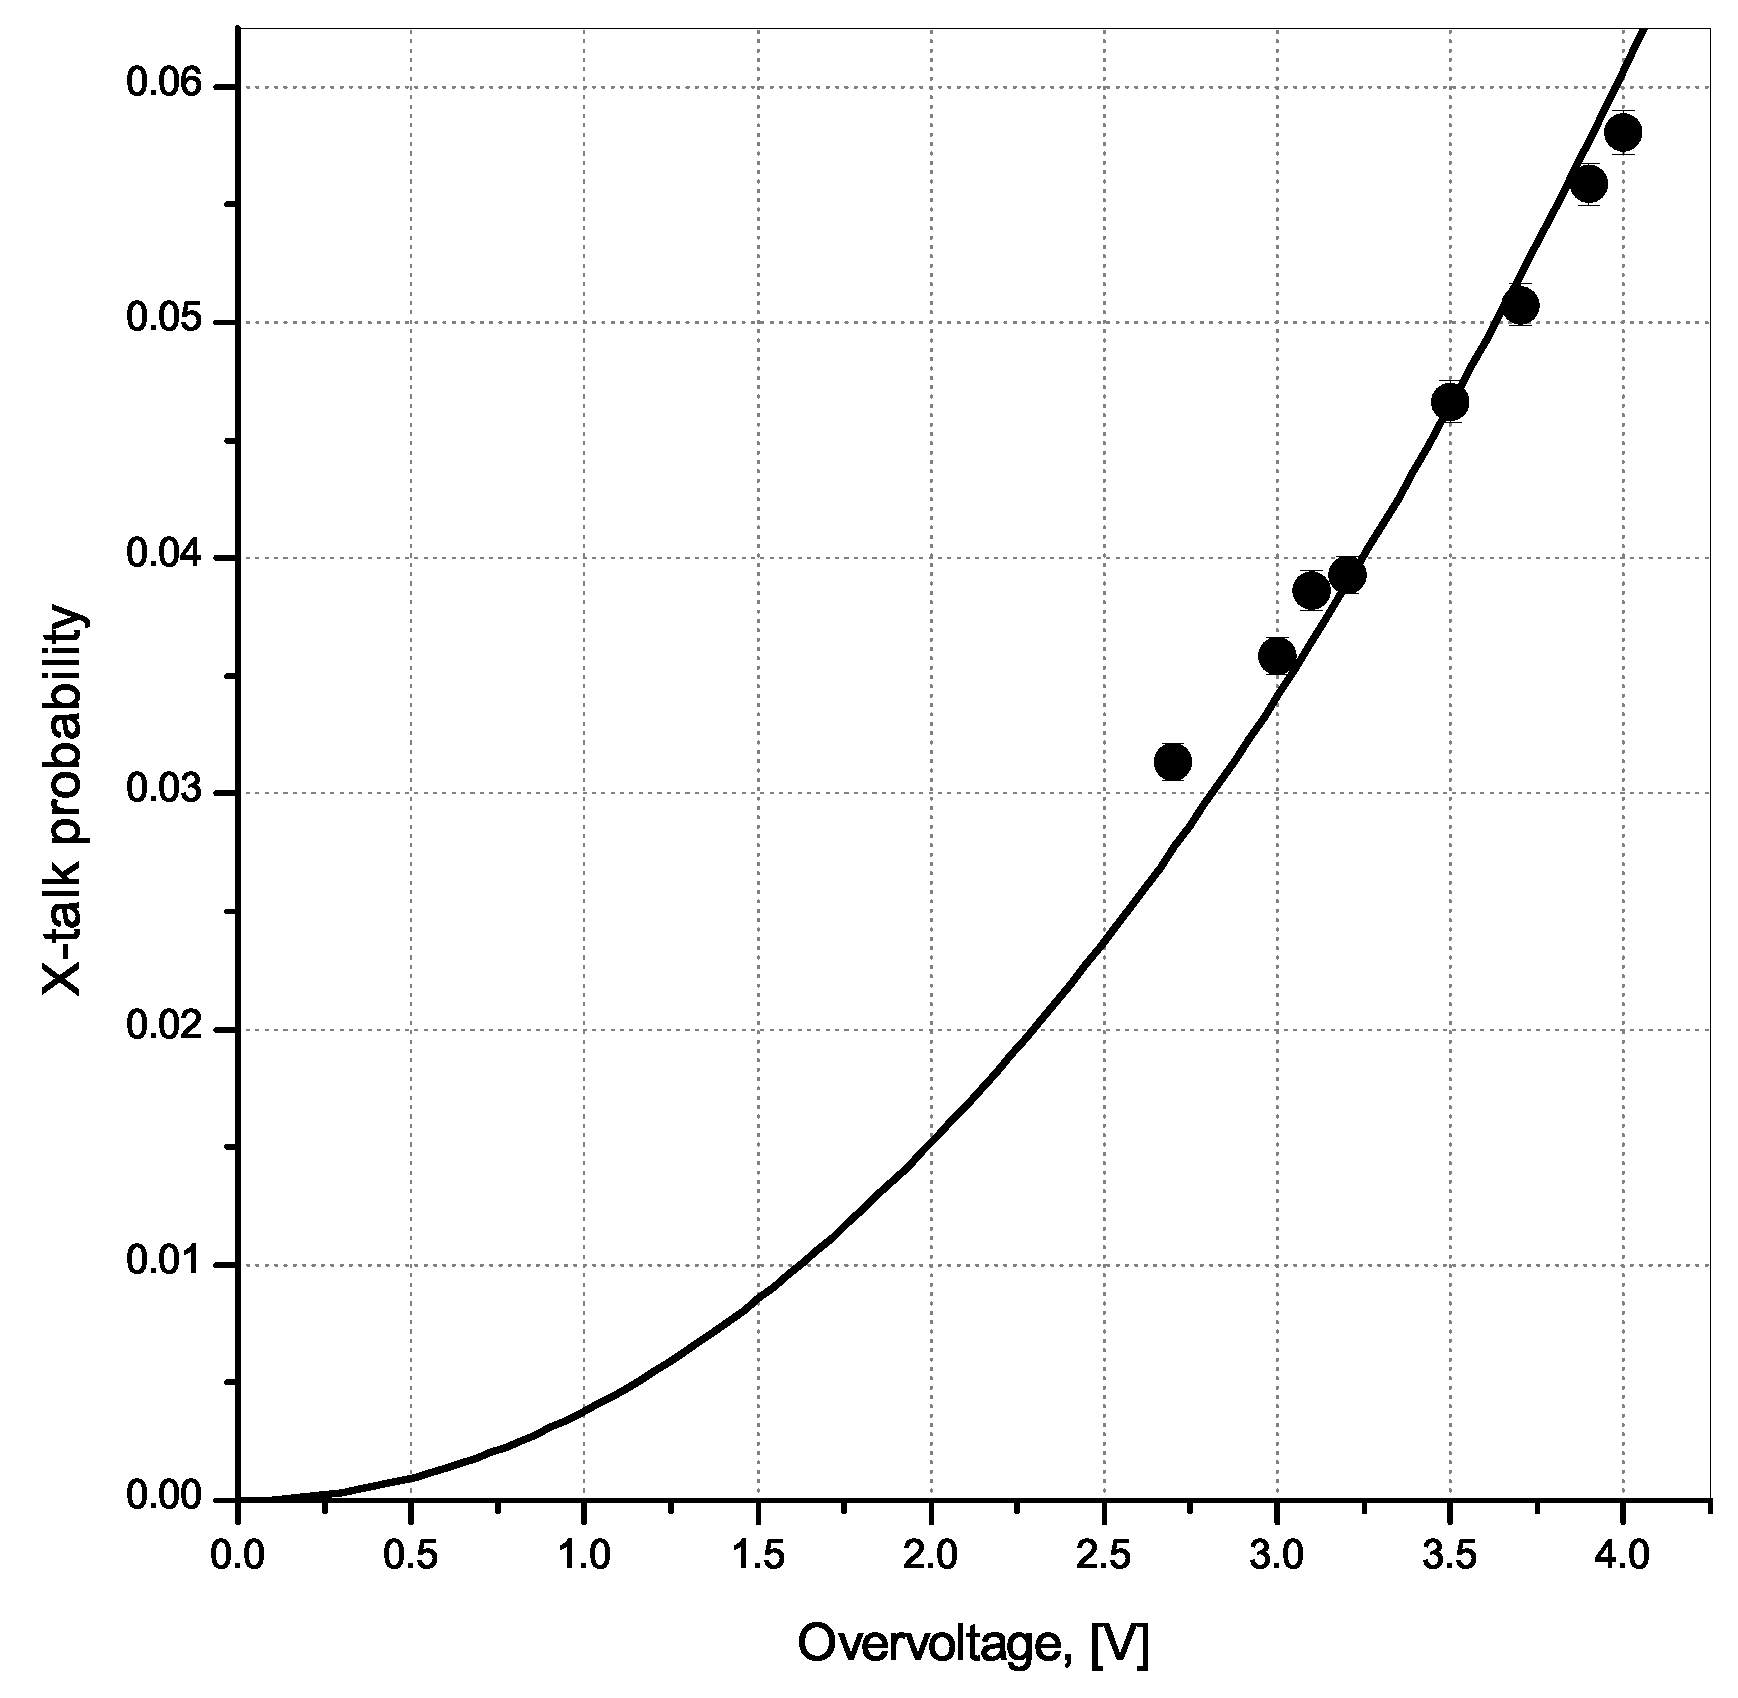
\includegraphics[width=0.47\textwidth]{KETEK_PM1125NS_SB0_x-tlak_vs_V_eng}
\\
\parbox[t]{0.47\textwidth}{\caption{The dependence of the cross-talk probability on an overvoltage at a fixed temperature for
Hamamatsu S13360-3050CS. The data were approximated by a quadratic function.}
\label{image:Hamamatsu_S13360-3050CS_xtalk_vs_V_rus}}
\hfill
\parbox[t]{0.47\textwidth}{\caption{The dependence of the cross-talk probability on an overvoltage at a fixed temperature for
KETEK PM1125NS-SB0. The data were approximated by a quadratic function.}
\label{image:KETEK_PM1125NS_SB0_x-tlak_vs_V_rus}}
\end{figure}

Based on the experimental data, it can be concluded that the cross-talk probability is temperature independent.

\subsection{Checking the model of four nearest neighbors}
It noted the existence of SiPM, which do not correspond to the model of four nearest neighbors \cite{Modeling crosstalk in silicon photomultipliers}.
In the model of four nearest neighbors it is assumed that trigged cell can cause the triggering of only four nearest cells.
In this case, the cross-talk probability in the next cell $p$ is related to the full cross-talk probability $P_{x-talk}$ by the following equation
\begin{eqnarray}\label{eq:p vs xtalk}
(1 - p)^4 = 1 - P_{X-talk}
\end{eqnarray}

Full cross-talk probability was calculated by the Eq.(\ref{eq:xtalk_general}).
Then $p$ value was calculated by Eq.(\ref{eq:p vs xtalk}).
It was calculated theoretical probability that due to cross-talk only one cell triggered \cite{Modeling crosstalk in silicon photomultipliers}: $p_{2 phe}^{theory} = 4 \cdot p \cdot (1 - p)^6$.
On the other hand it was calculated the experimental probability $p_{2 phe}^{exp}$ as the ratio of events number $N_{2 p.e.}$ to the total number of events,
where $N_{2 p.e.} \approx  N_{B_{1}} / (N_{A_{1}} + N_{B_{1}} + N_{C_{1}})$.
As a result of measurements, it was found that the ratio $p_{2 phe}^{exp} / p_{2 phe}^{theory}$ for Hamamatsu S10362-11-100C varies from 1 to 1.08 depending on temperature and overvoltage, and for Hamamatsu S13360-3050CS and KETEK PM1125NS-SB0 this ratio varies from 0.98 to 1.02.
Thus it can be concluded that the model of four nearest neighbors works well for considered SiPMs.

\subsection{After-pulses}

As a result of spectrum approximation we fond also probabilities and time constants for after-pulses.
The obtained data are shown in Fig.~\ref{image:Hamamatsu_S10362-11-100C_p_f_vs_T}, \ref{image:Hamamatsu_S10362-11-100C_p_f_vs_V}, \ref{image:Hamamatsu_S10362-11-100C_p_s_vs_T}, \ref{image:Hamamatsu_S10362-11-100C_p_s_vs_V}, \ref{image:Hamamatsu_S10362-11-100C_tau_f_vs_T}, \ref{image:Hamamatsu_S10362-11-100C_tau_f_vs_V}, \ref{image:Hamamatsu_S10362-11-100C_tau_s_vs_T},
 \ref{image:Hamamatsu_S10362-11-100C_tau_s_vs_V}, \ref{image:Hamamatsu_S13360-3050CS_p_f_vs_V_rus}, \ref{image:Hamamatsu_S13360-3050CS_tau_s_vs_V}, \ref{image:KETEK_PM1125NS_SB0_p_f_vs_V_rus}, \ref{image:KETEK_PM1125NS_SB0_tau_f_vs_V_rus}.

\begin{figure}[h]
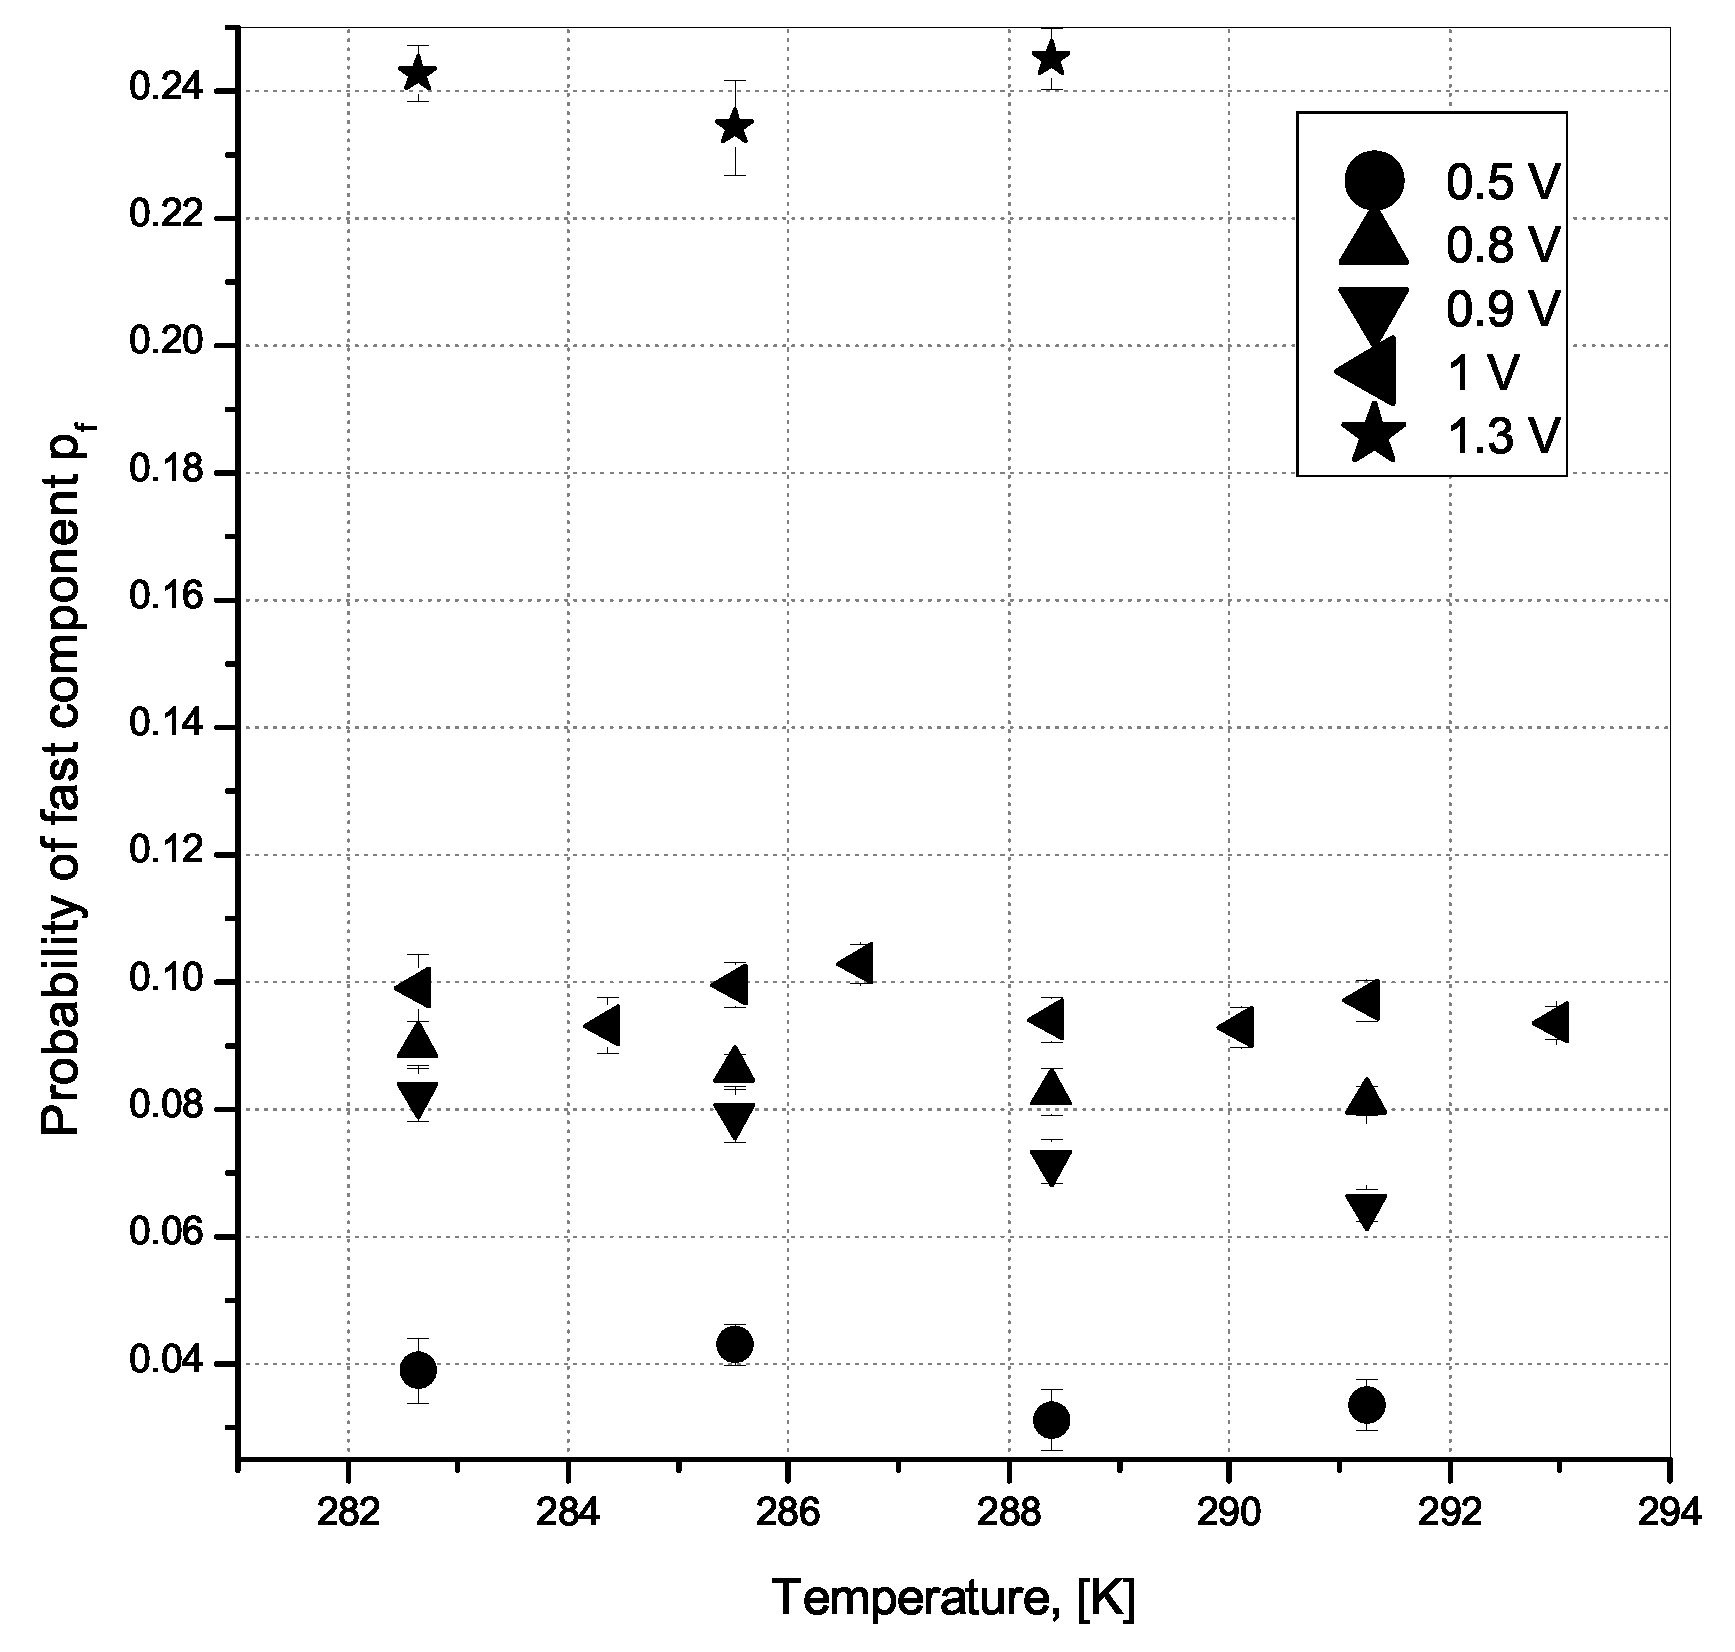
\includegraphics[width=0.47\textwidth]{Hamamatsu_S10362-11-100C_p_f_vs_T_eng}
\hfill
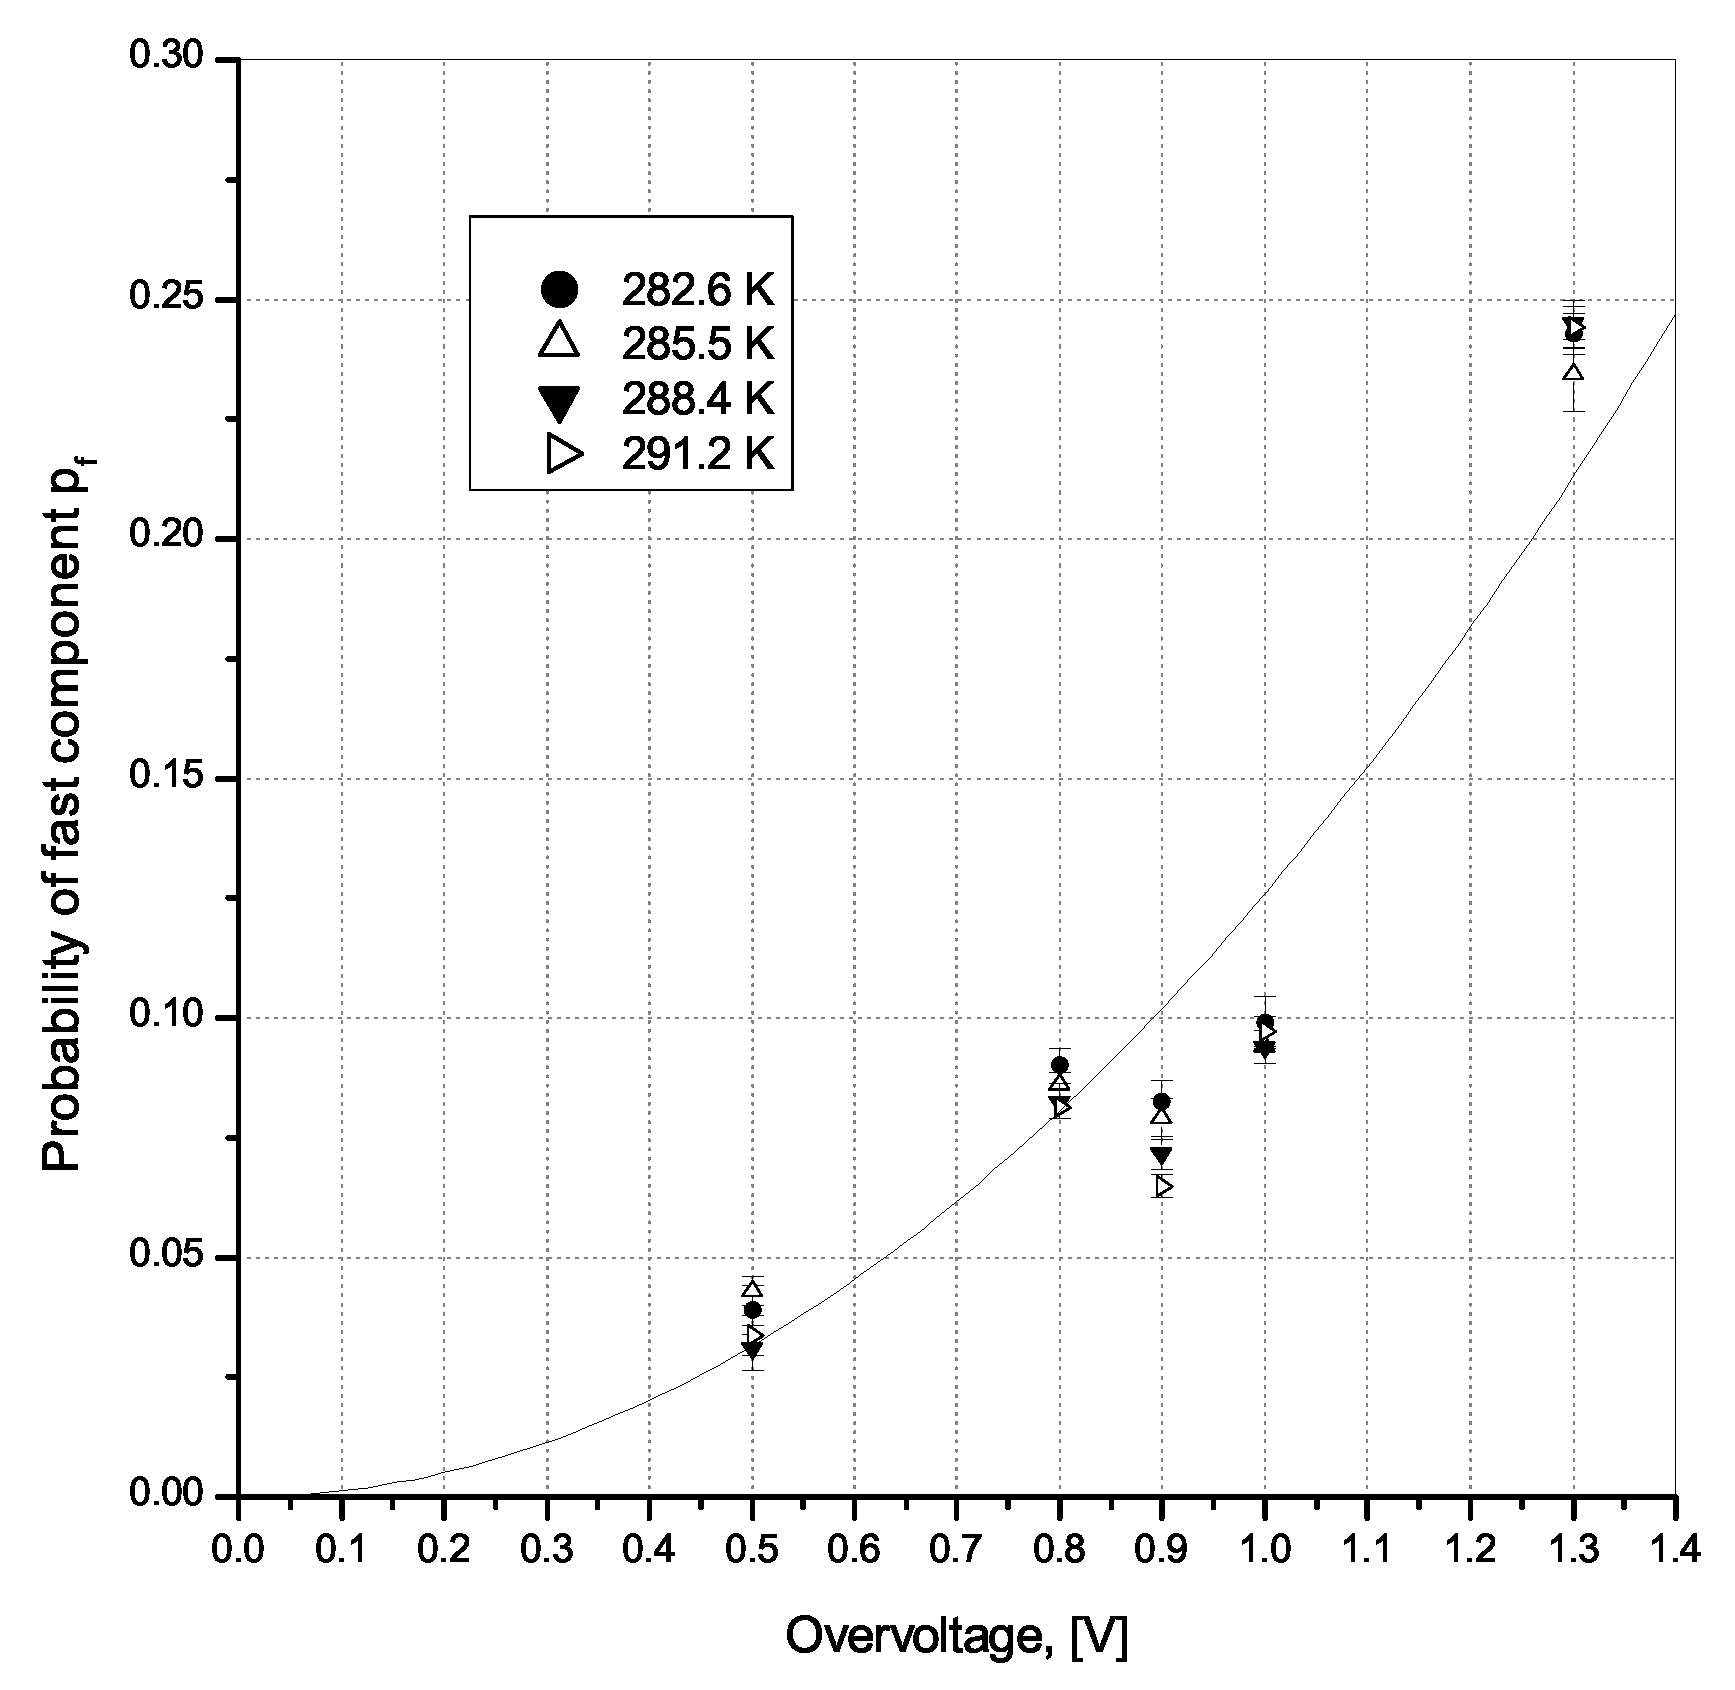
\includegraphics[width=0.47\textwidth]{Hamamatsu_S10362-11-100C_p_f_vs_V_eng}
\\
\parbox[t]{0.47\textwidth}{\caption{The dependence of the fast component probability $p_{f}$ for after-pulse on the temperature at fixed overvoltage for
Hamamatsu S10362-11-100C.}
\label{image:Hamamatsu_S10362-11-100C_p_f_vs_T}}
\hfill
\parbox[t]{0.47\textwidth}{\caption{The dependence of the fast component probability $p_{f}$ for after-pulse on the overvoltage at fixed temperature for
Hamamatsu S10362-11-100C. The data were approximated by a quadratic function.}
\label{image:Hamamatsu_S10362-11-100C_p_f_vs_V}}
\end{figure}

\begin{figure}[h]
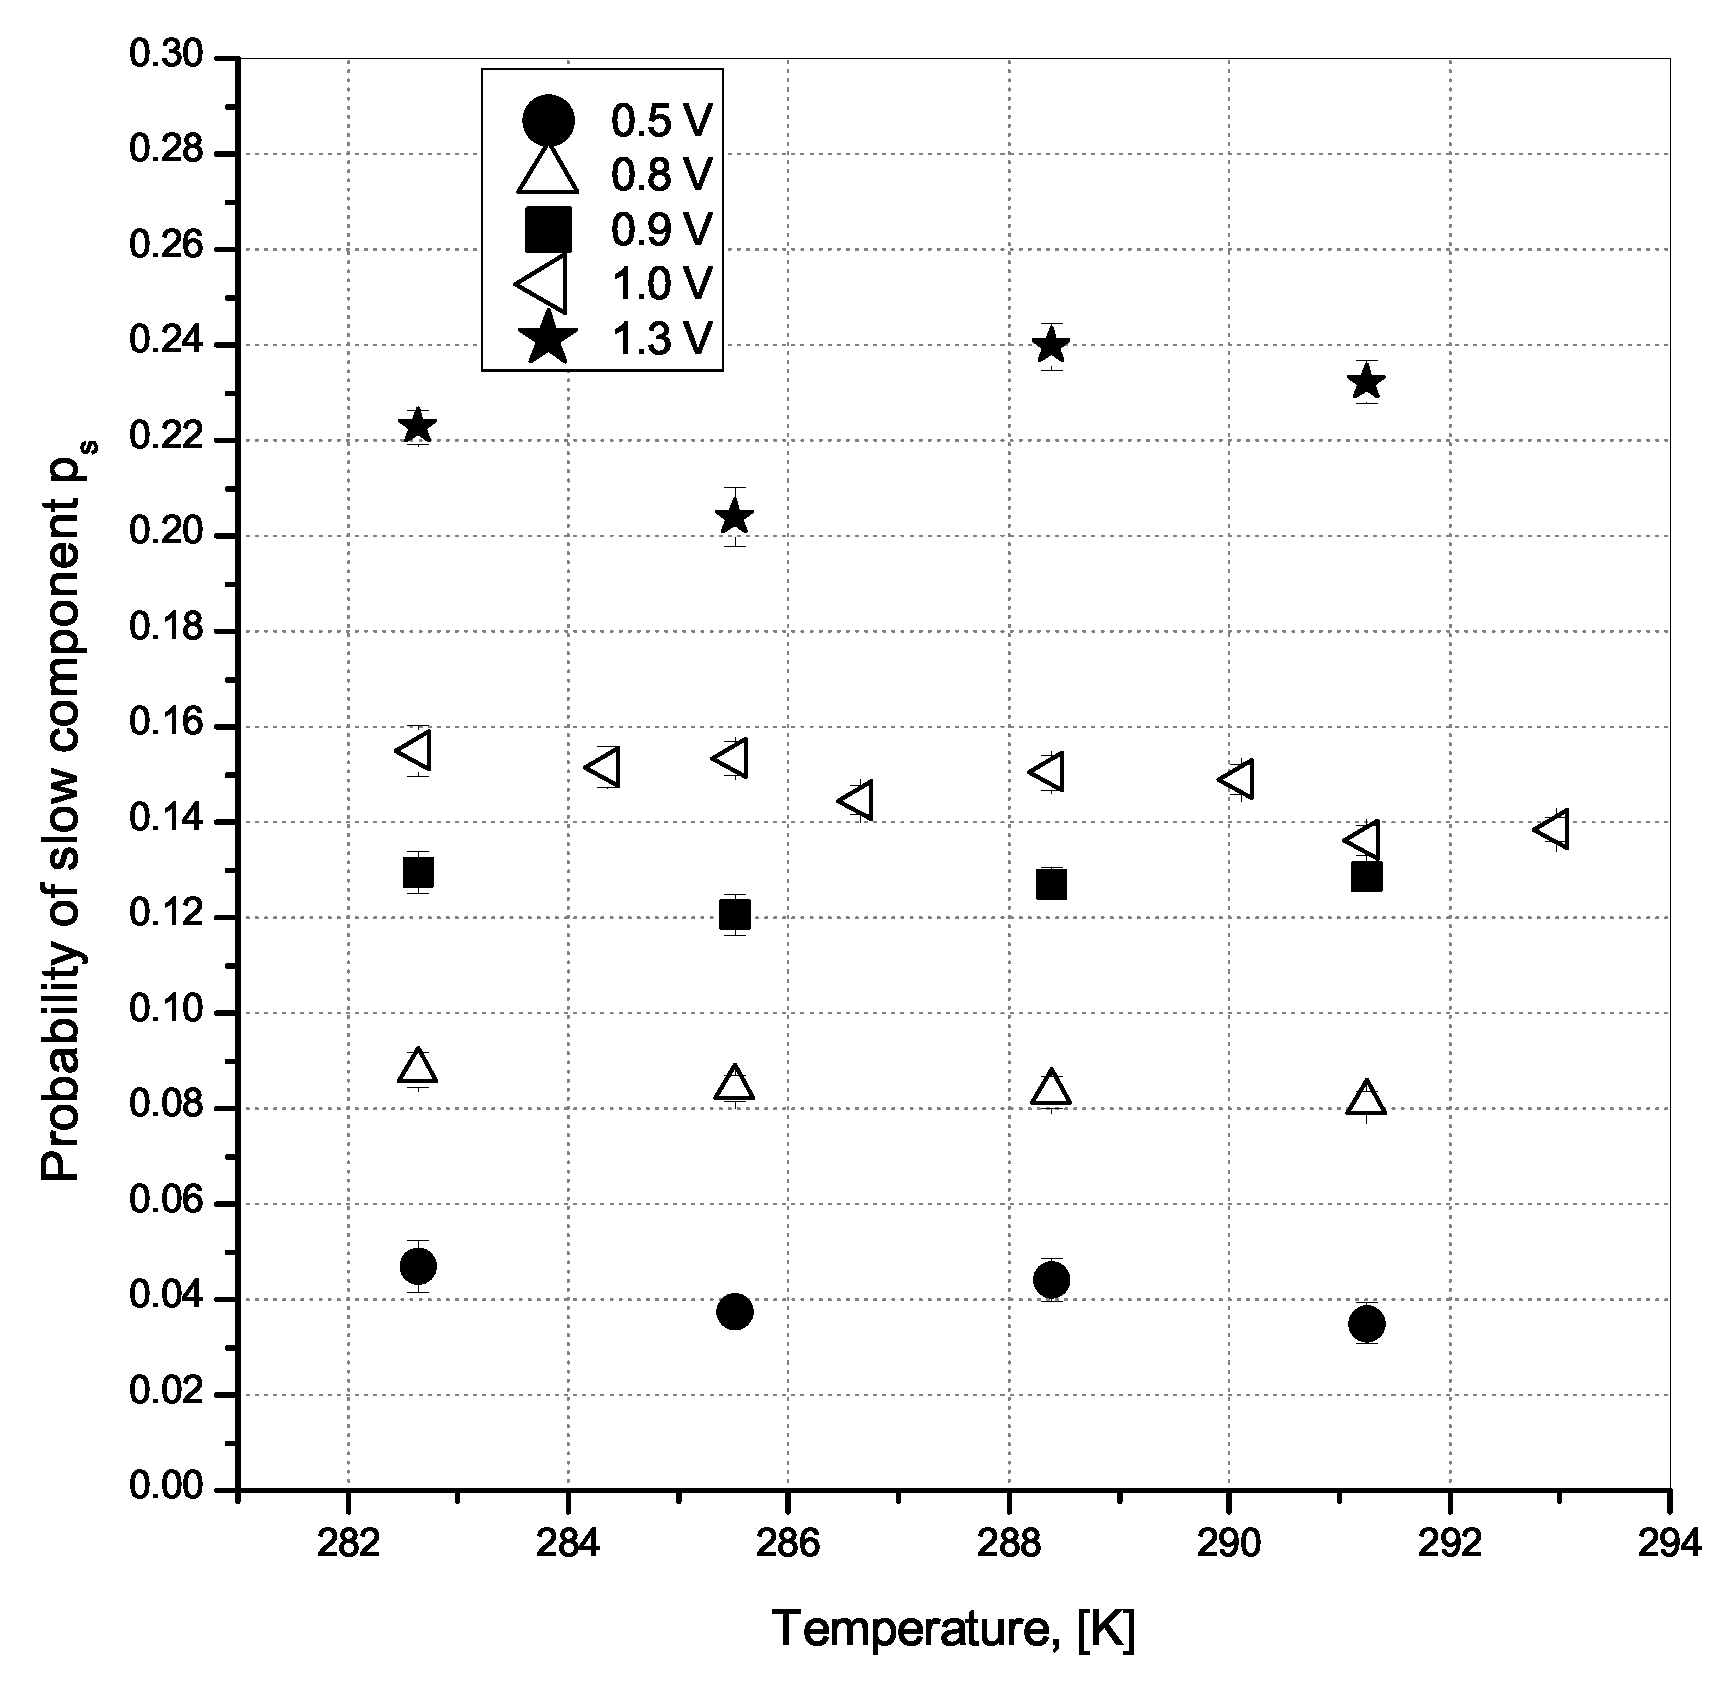
\includegraphics[width=0.47\textwidth]{Hamamatsu_S10362-11-100C_p_s_vs_T_eng}
\hfill
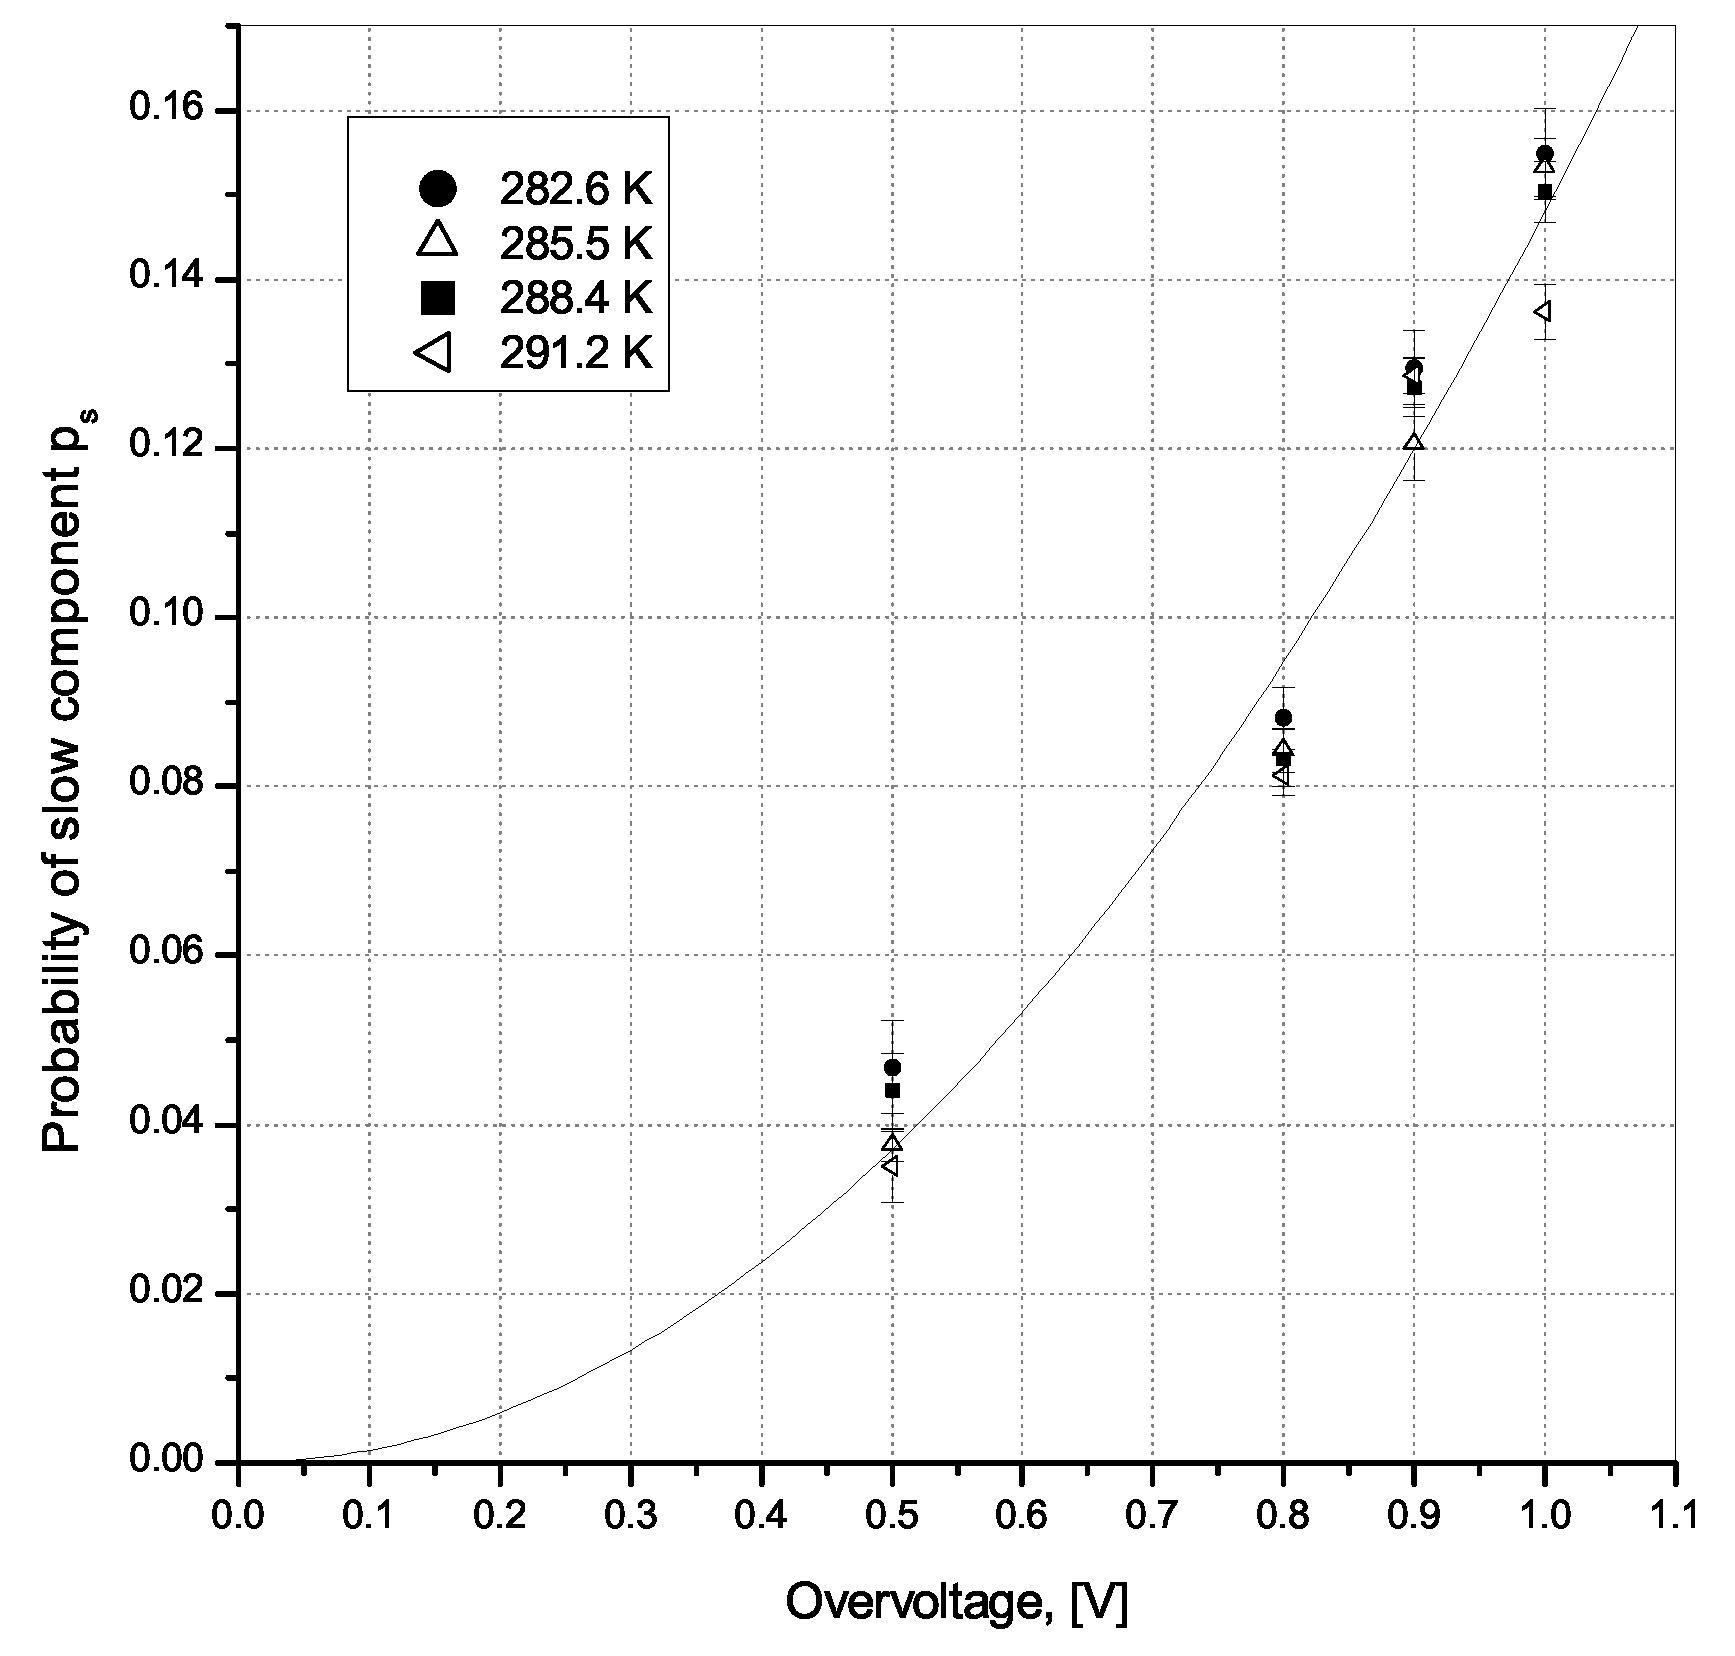
\includegraphics[width=0.47\textwidth]{Hamamatsu_S10362-11-100C_p_s_vs_V_eng}
\\
\parbox[t]{0.47\textwidth}{\caption{The dependence of the slow component probability $p_{s}$ for after-pulse on the temperature at fixed overvoltage for
Hamamatsu S10362-11-100C.}
\label{image:Hamamatsu_S10362-11-100C_p_s_vs_T}}
\hfill
\parbox[t]{0.47\textwidth}{\caption{The dependence of the slow component probability $p_{s}$ for after-pulse on the overvoltage at fixed temperature for
Hamamatsu S10362-11-100C. The data were approximated by a quadratic function.}
\label{image:Hamamatsu_S10362-11-100C_p_s_vs_V}}
\end{figure}

\begin{figure}[h]
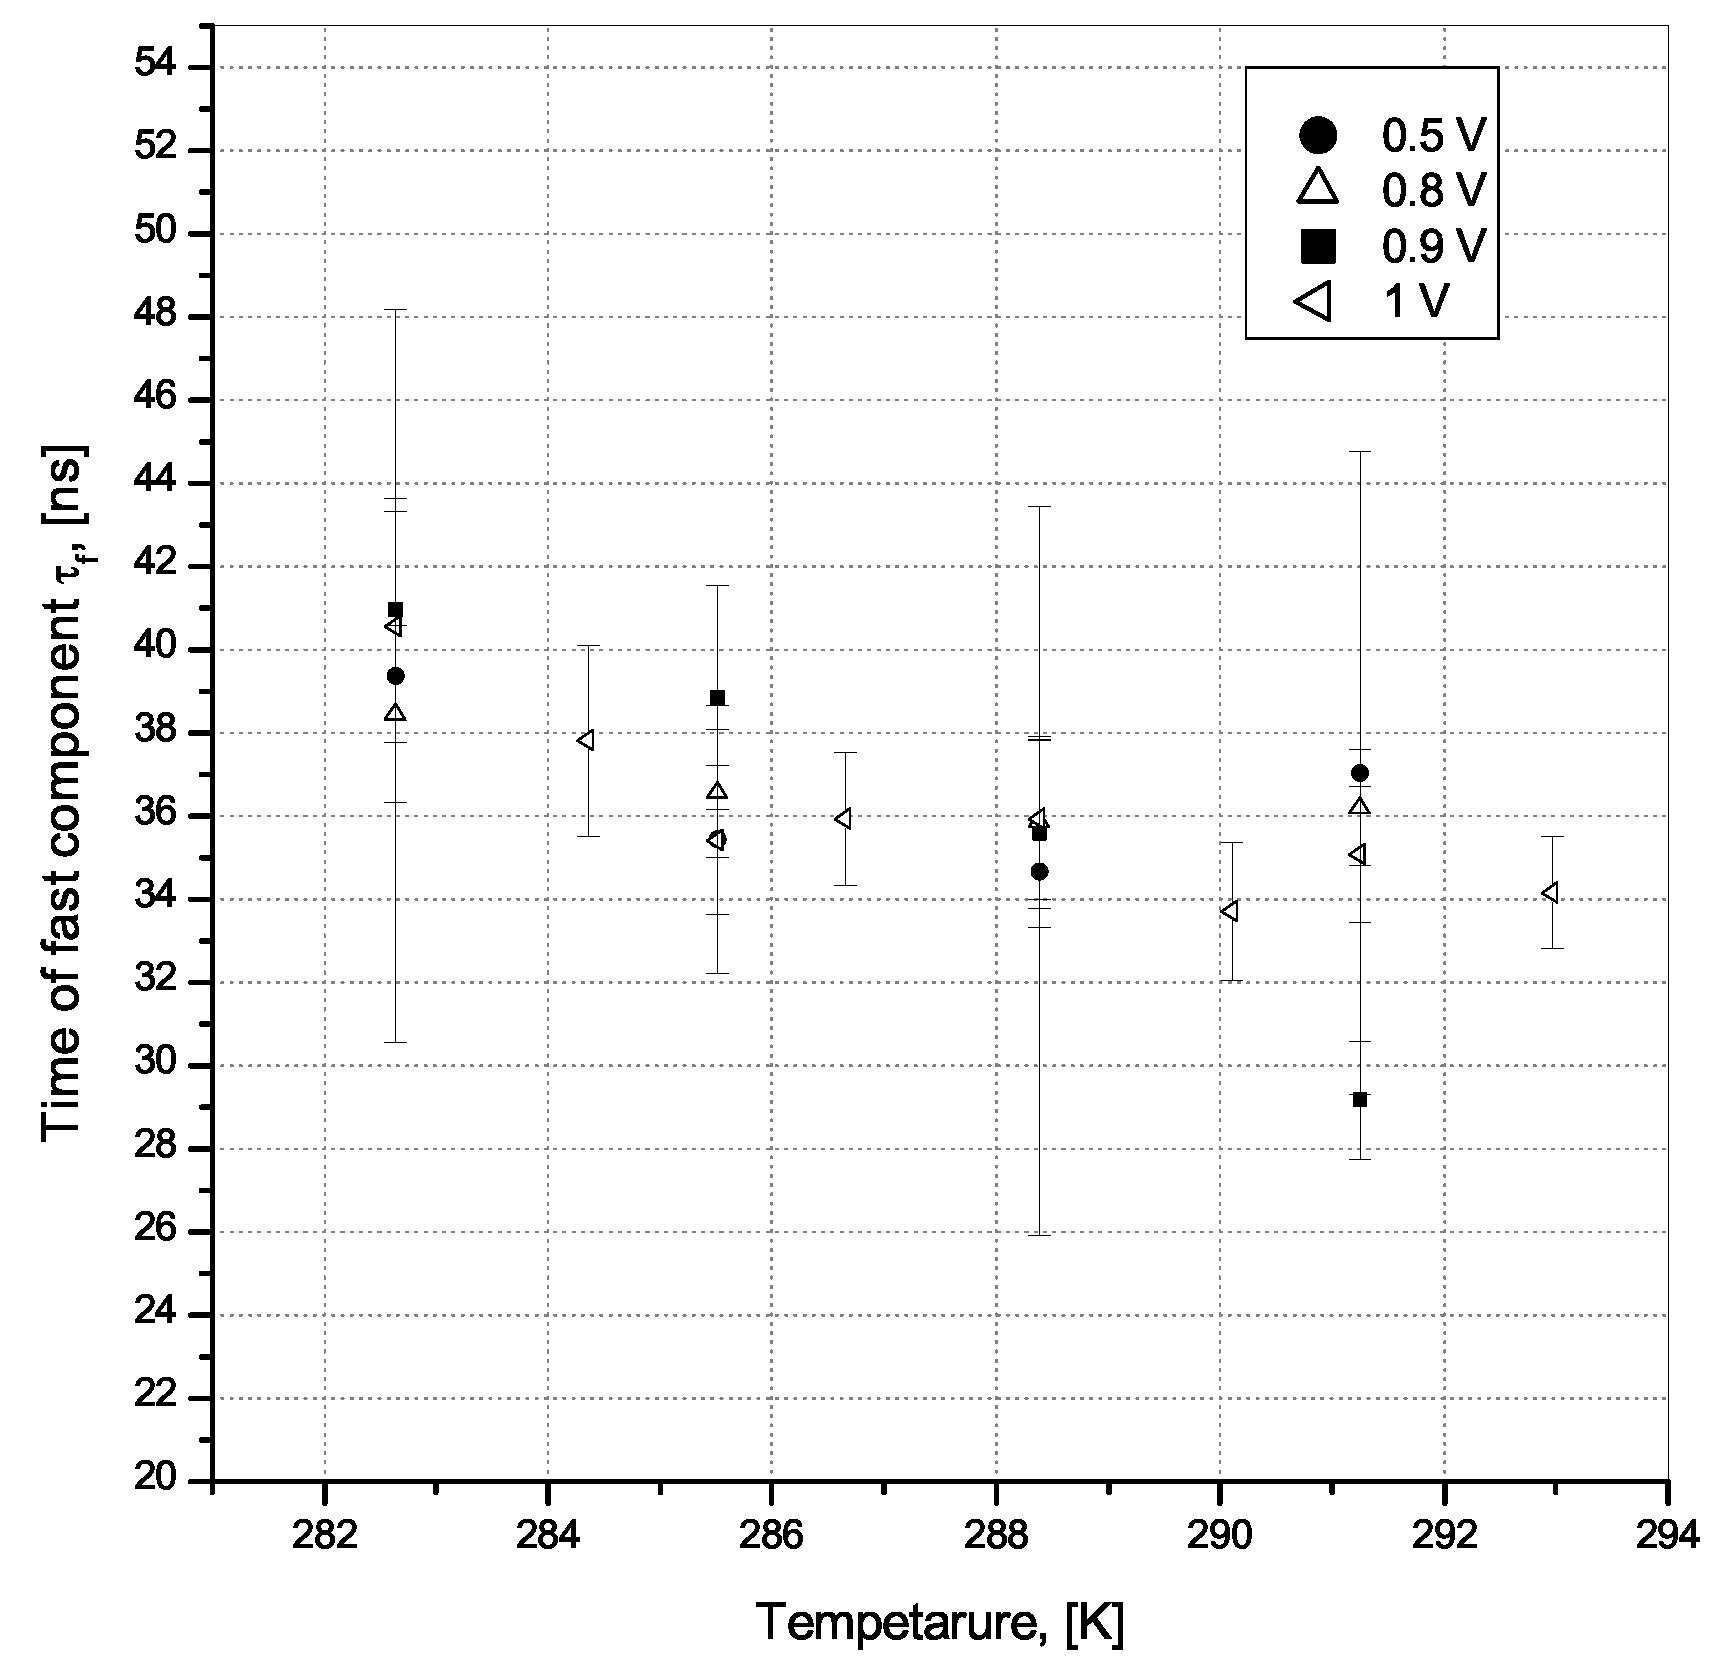
\includegraphics[width=0.47\textwidth]{Hamamatsu_S10362-11-100C_tau_f_vs_T_eng}
\hfill
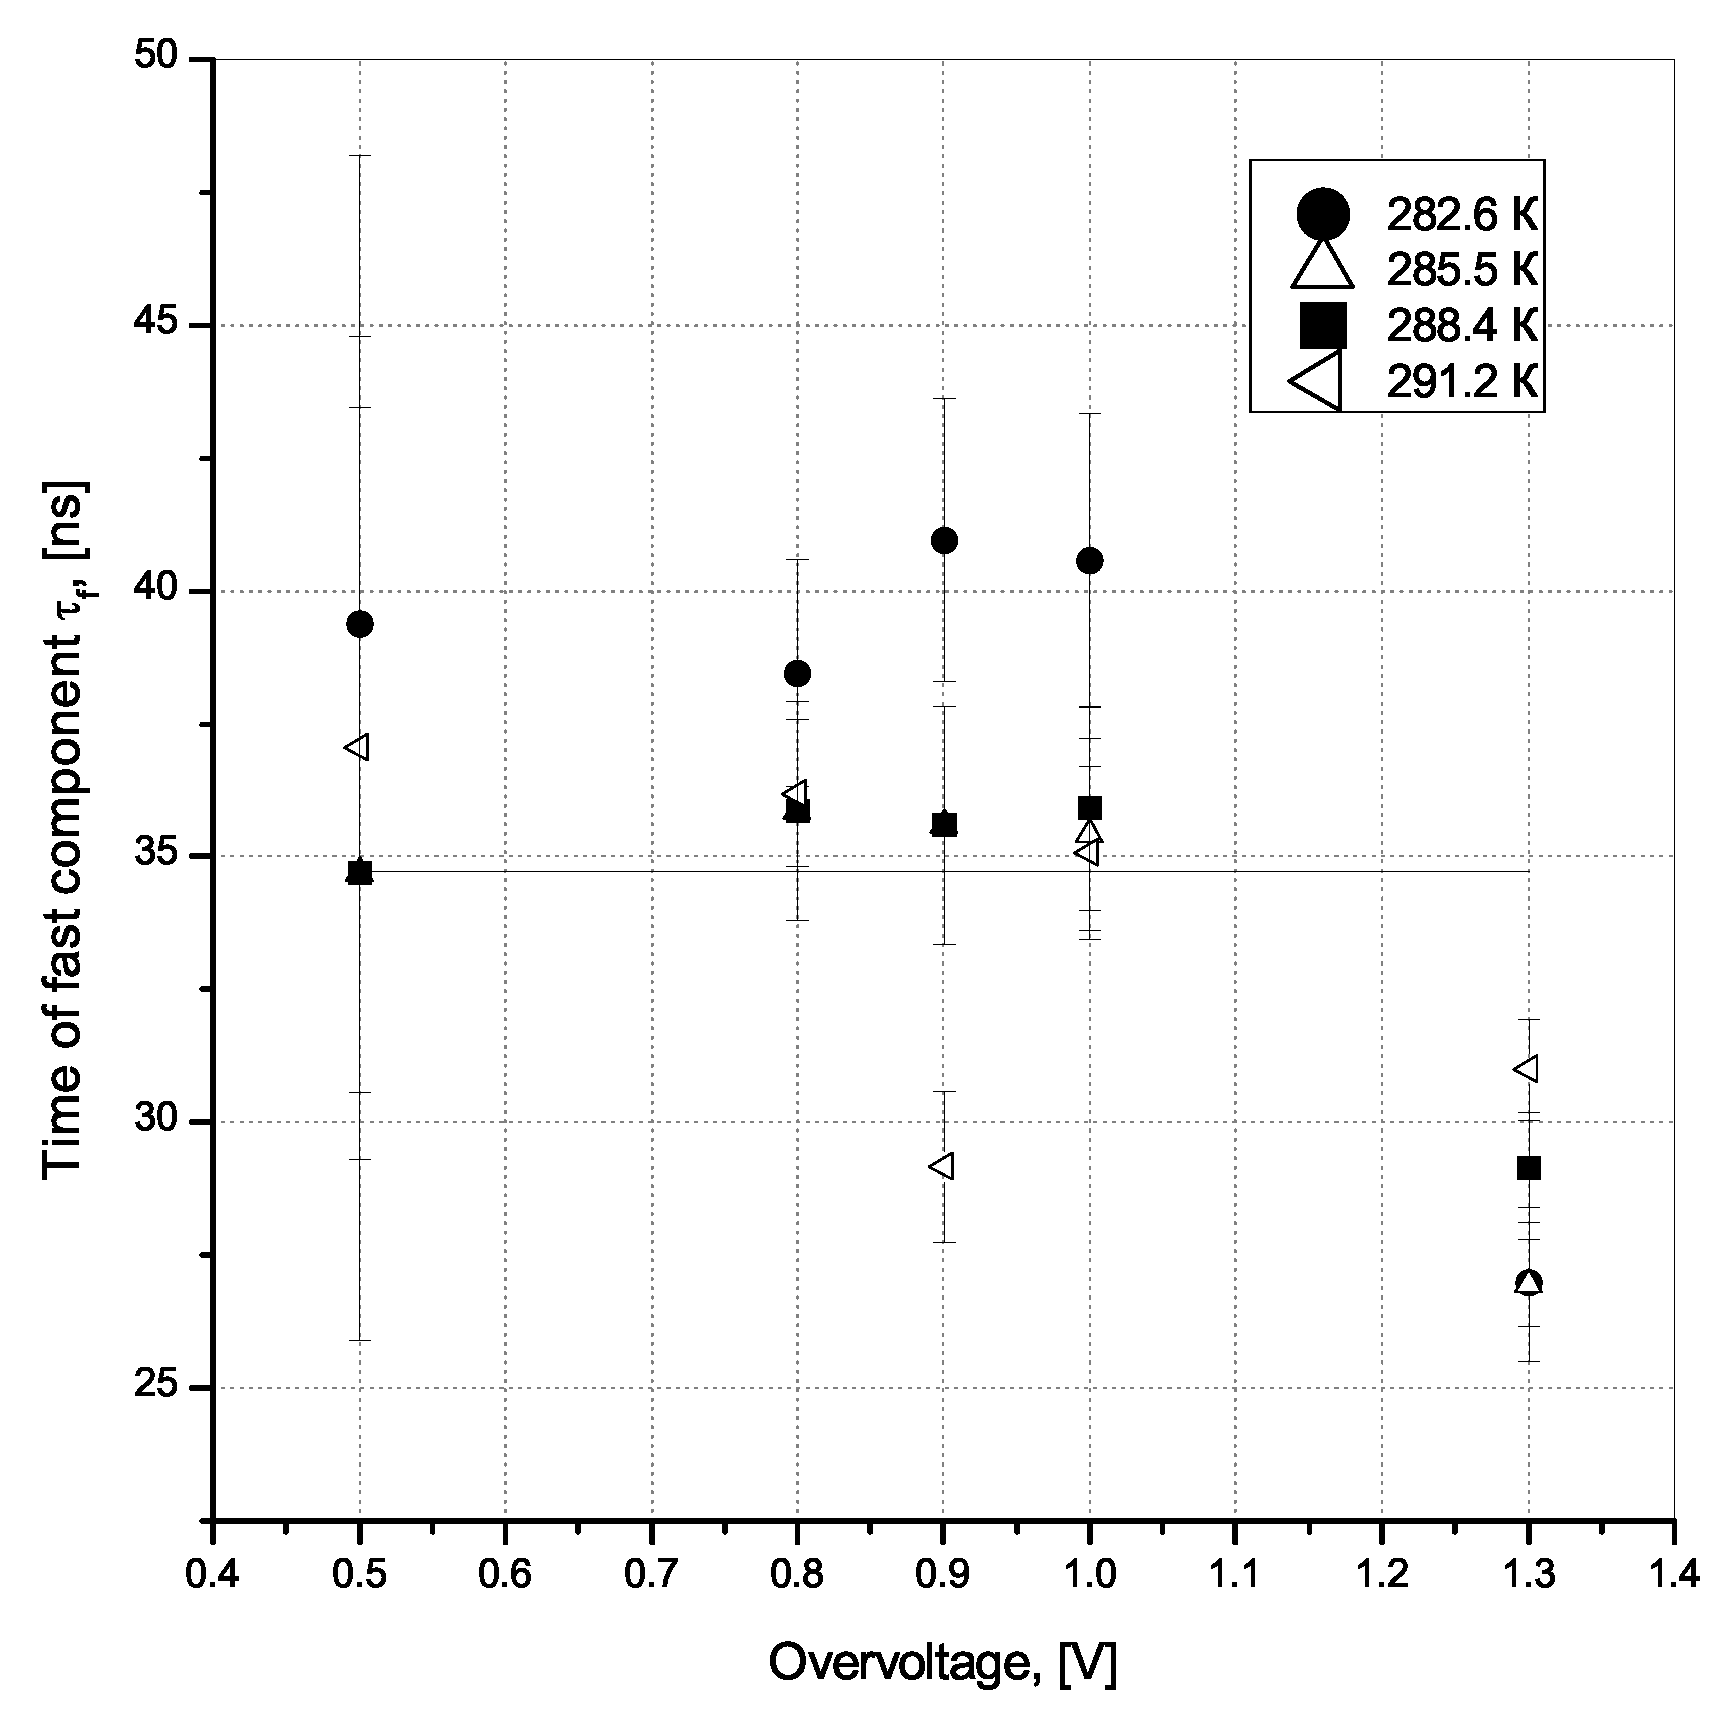
\includegraphics[width=0.47\textwidth]{Hamamatsu_S10362-11-100C_tau_f_vs_V_eng}
\\
\parbox[t]{0.47\textwidth}{\caption{The dependence of the fast time constant $\tau_{f}$ for after-pulse on the temperature at fixed overvoltage for
Hamamatsu S10362-11-100C.}
\label{image:Hamamatsu_S10362-11-100C_tau_f_vs_T}}
\hfill
\parbox[t]{0.47\textwidth}{\caption{The dependence of the fast time constant $\tau_{f}$ for after-pulse on the overvoltage at fixed temperature for
Hamamatsu S10362-11-100C.}
\label{image:Hamamatsu_S10362-11-100C_tau_f_vs_V}}
\end{figure}

%\if 0
\begin{figure}[h]
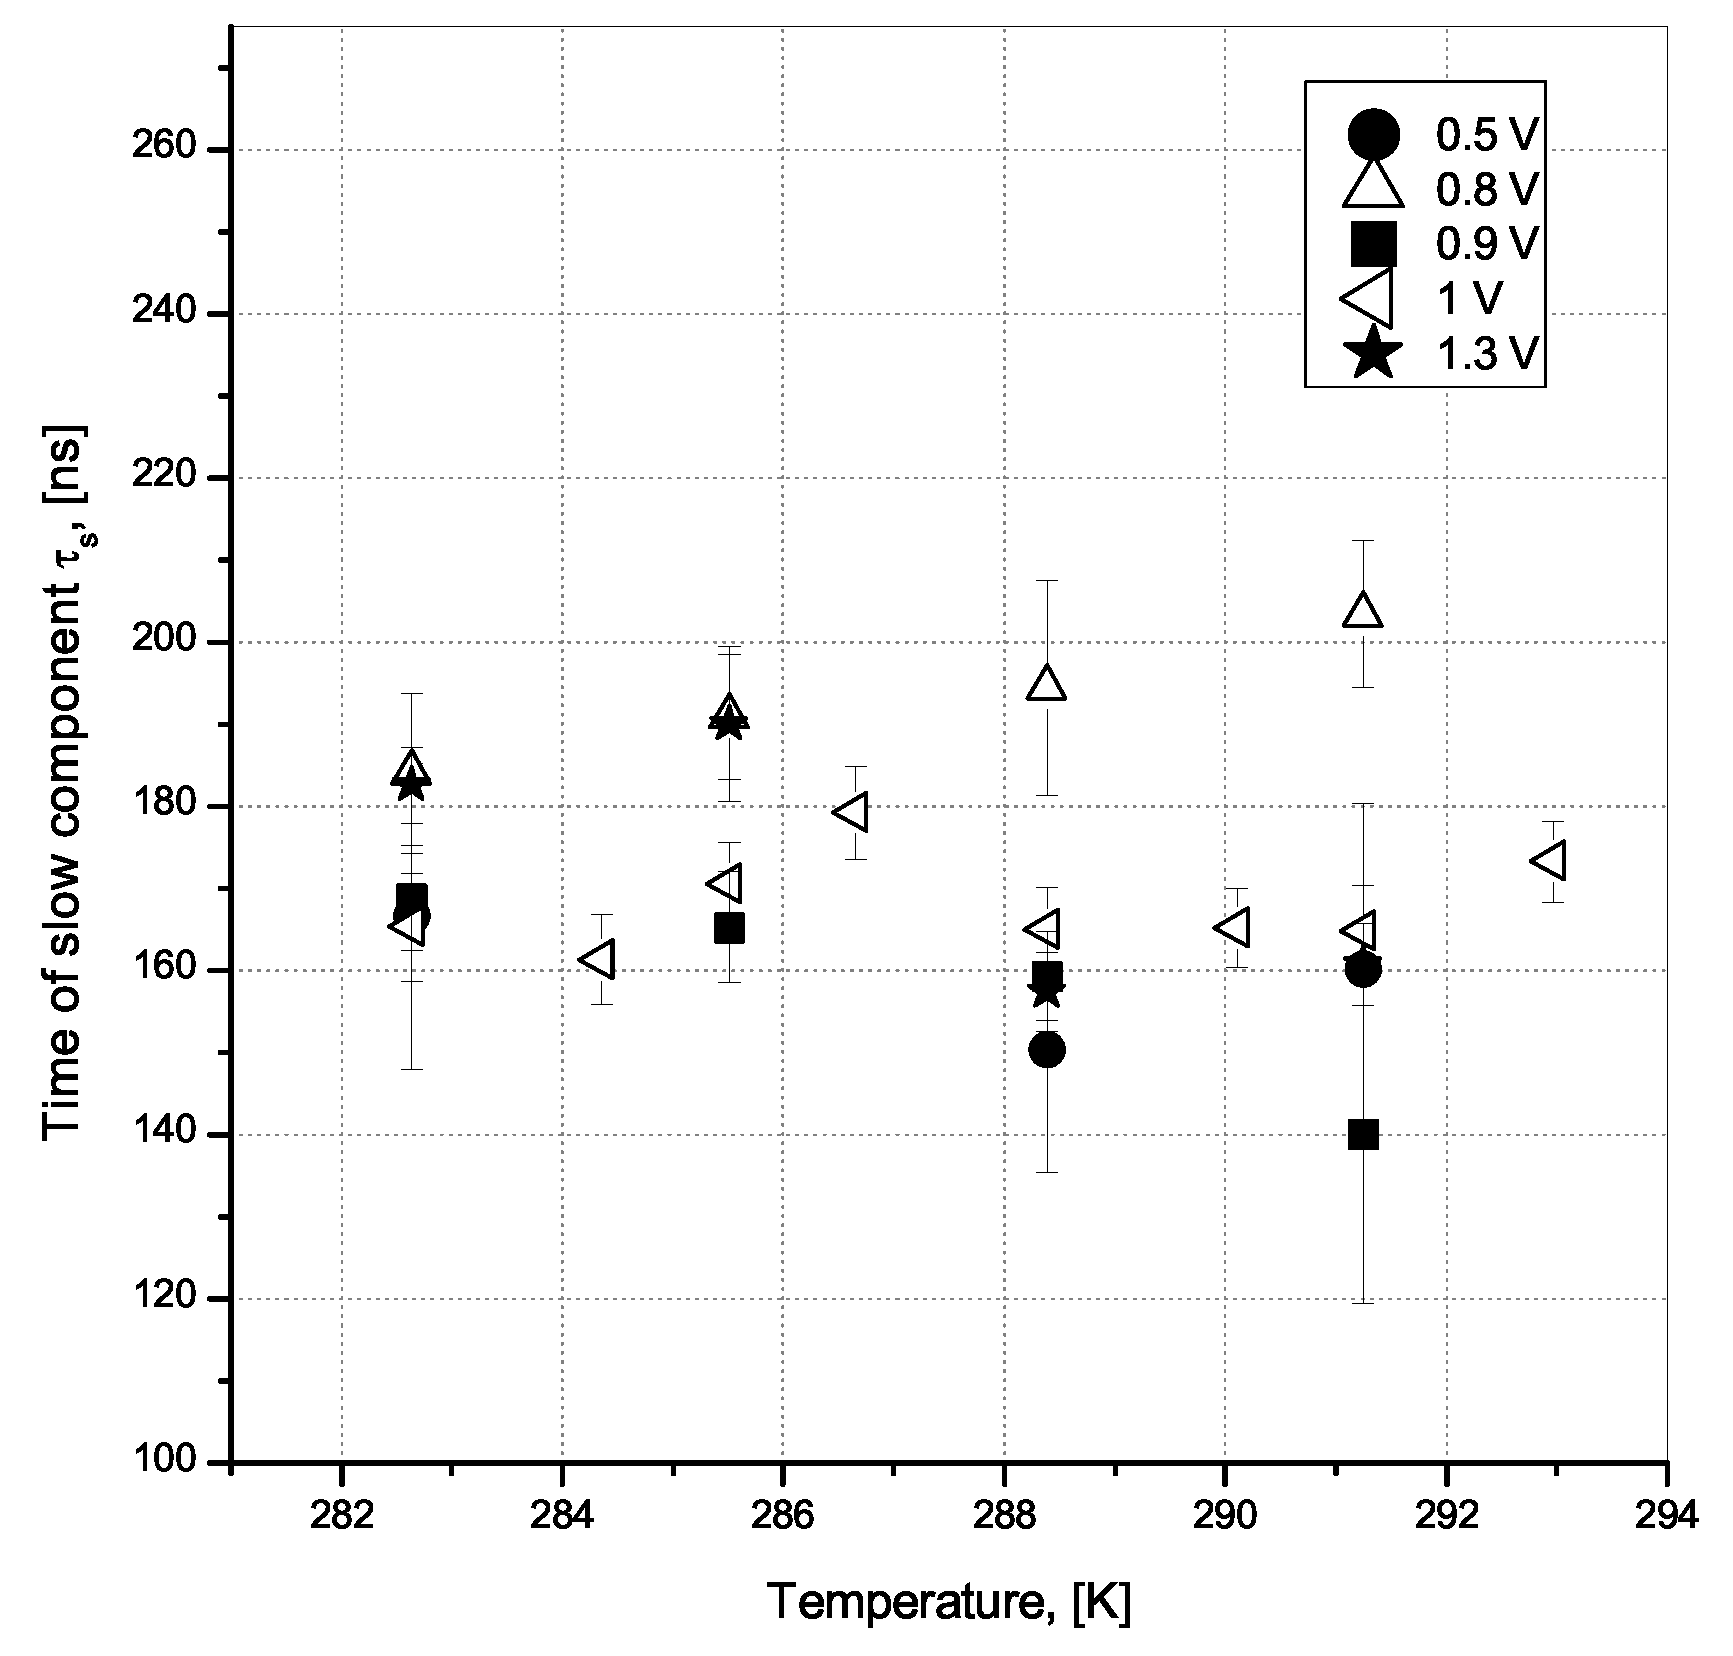
\includegraphics[width=0.47\textwidth]{Hamamatsu_S10362-11-100C_tau_s_vs_T_eng}
\hfill
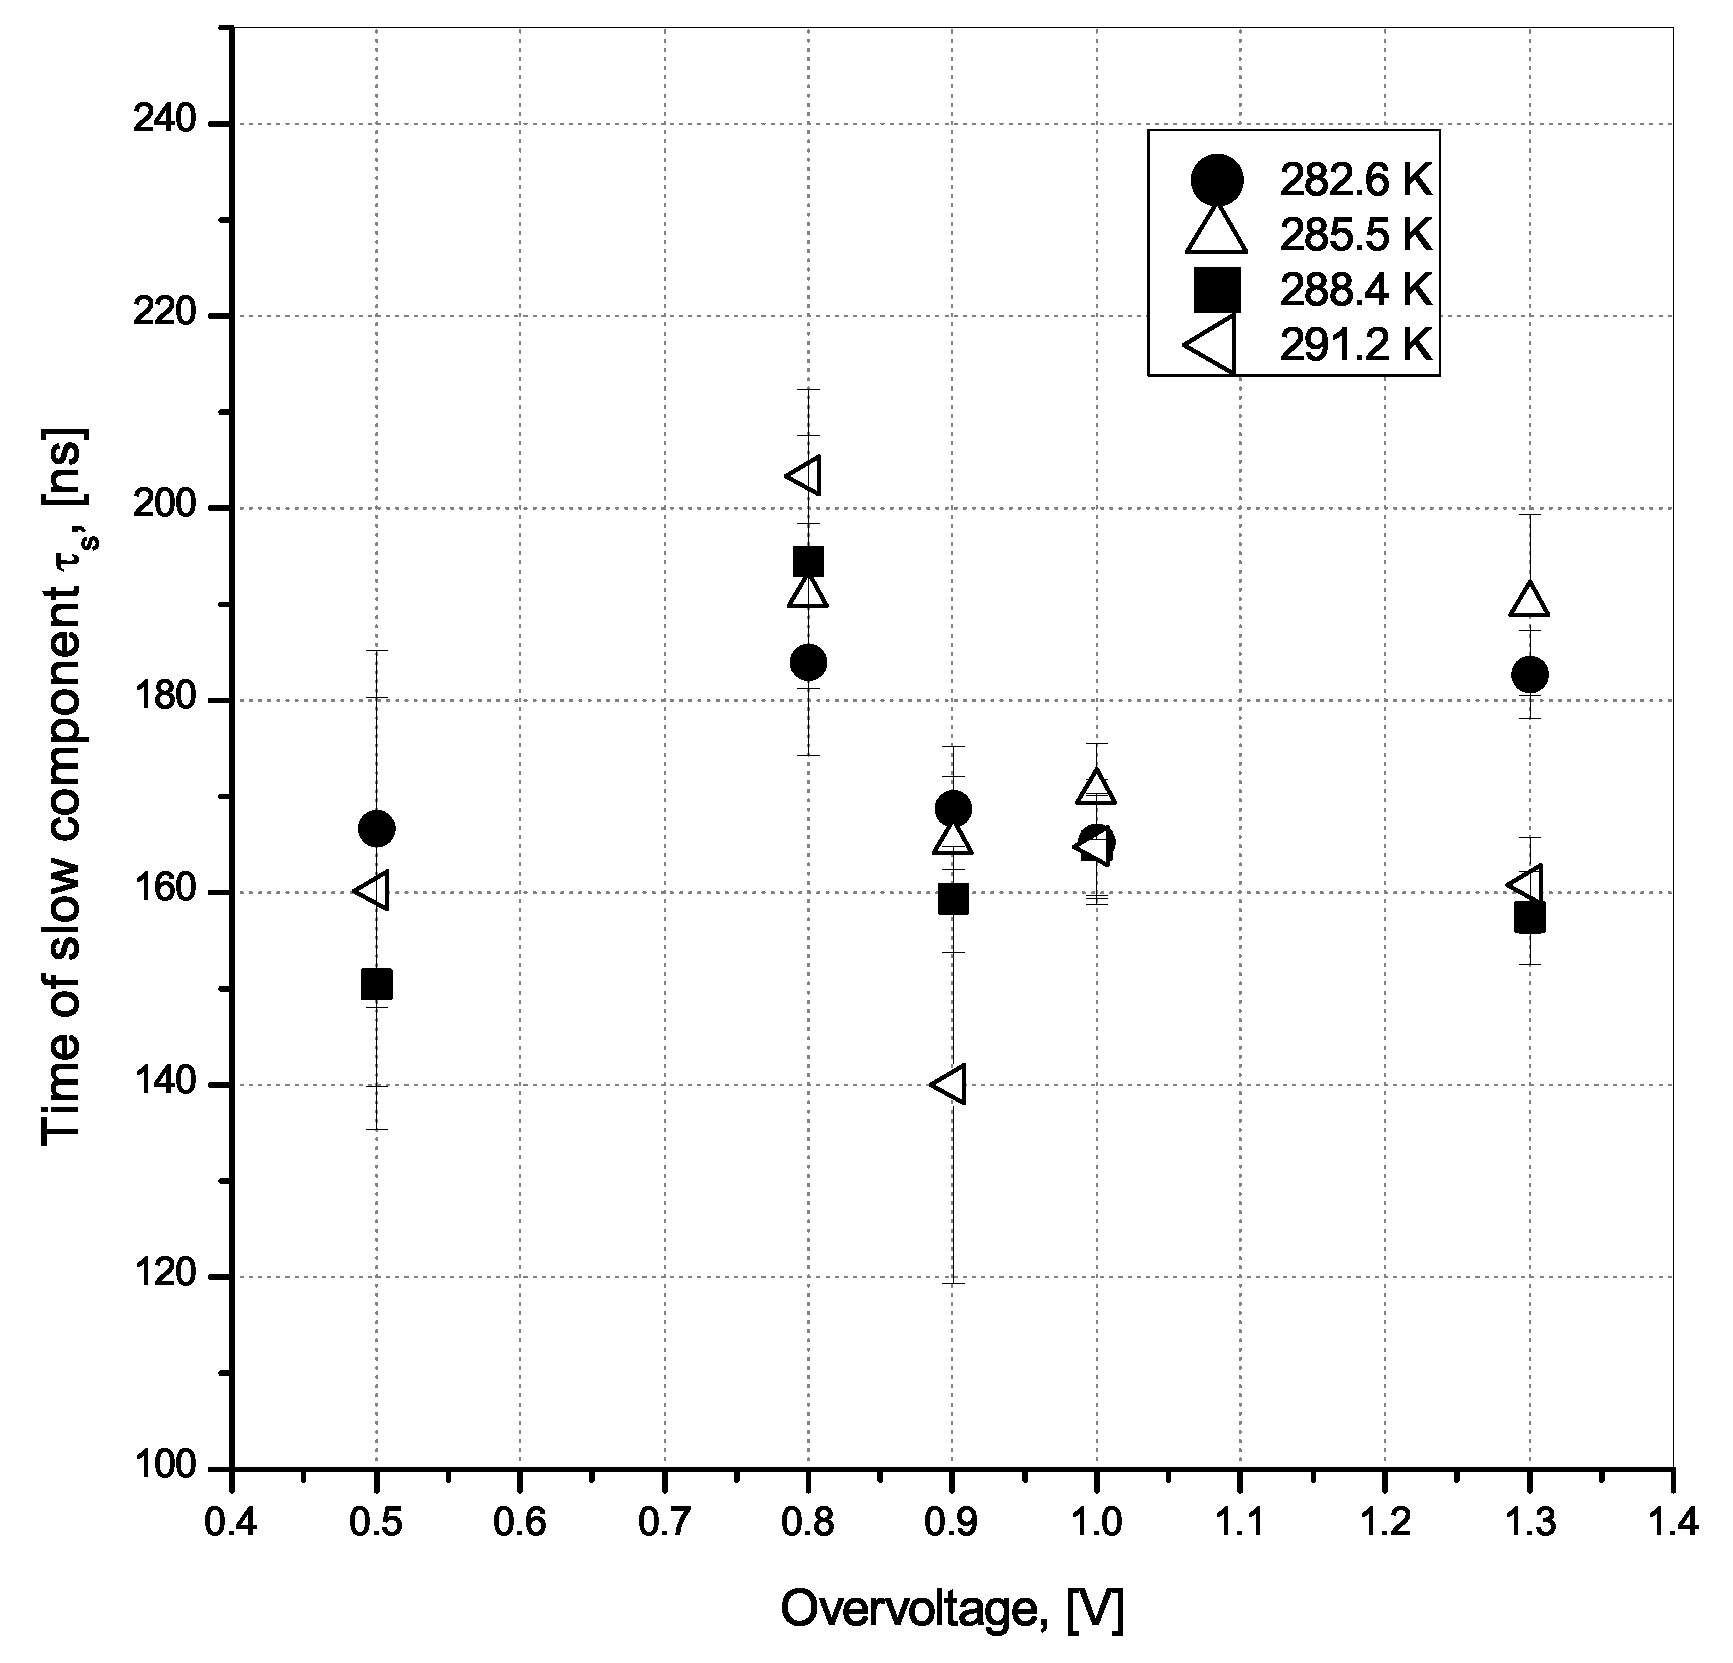
\includegraphics[width=0.47\textwidth]{Hamamatsu_S10362-11-100C_tau_s_vs_V_eng}
\\
\parbox[t]{0.47\textwidth}{\caption{The dependence of the slow time constant $\tau_{s}$ for after-pulse on the temperature at fixed overvoltage for
Hamamatsu S10362-11-100C.}
\label{image:Hamamatsu_S10362-11-100C_tau_s_vs_T}}
\hfill
\parbox[t]{0.47\textwidth}{\caption{The dependence of the slow time constant $\tau_{s}$ for after-pulse on the overvoltage at fixed temperature for
Hamamatsu S10362-11-100C.}
\label{image:Hamamatsu_S10362-11-100C_tau_s_vs_V}}
\end{figure}
%\fi

\begin{figure}[h]
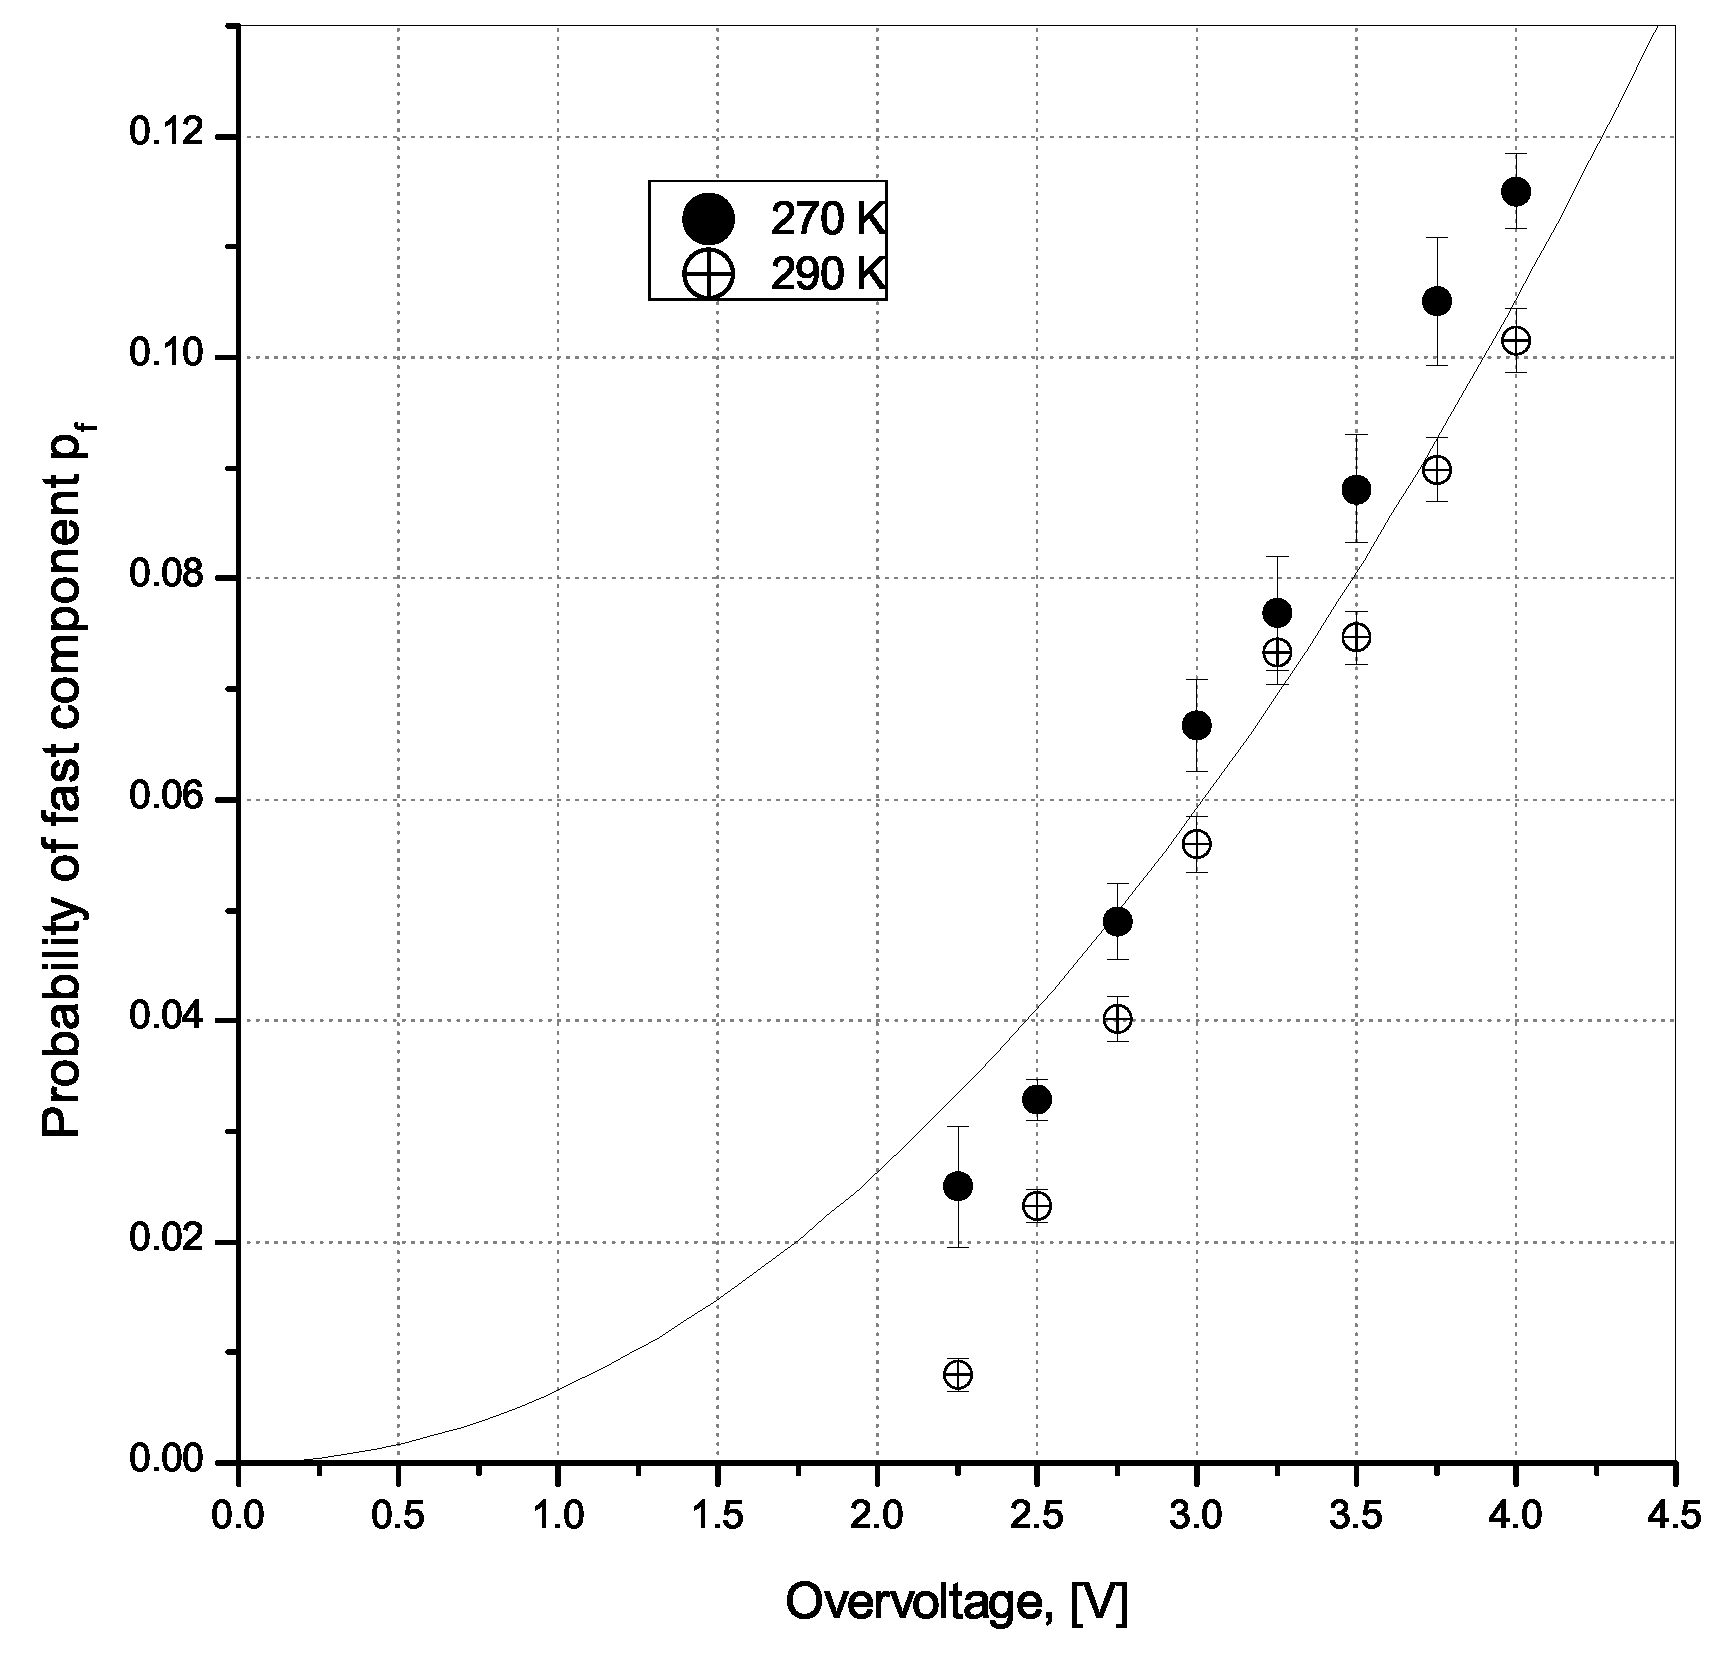
\includegraphics[width=0.47\textwidth]{Hamamatsu_S13360-3050CS_p_f_vs_V_eng}
\hfill
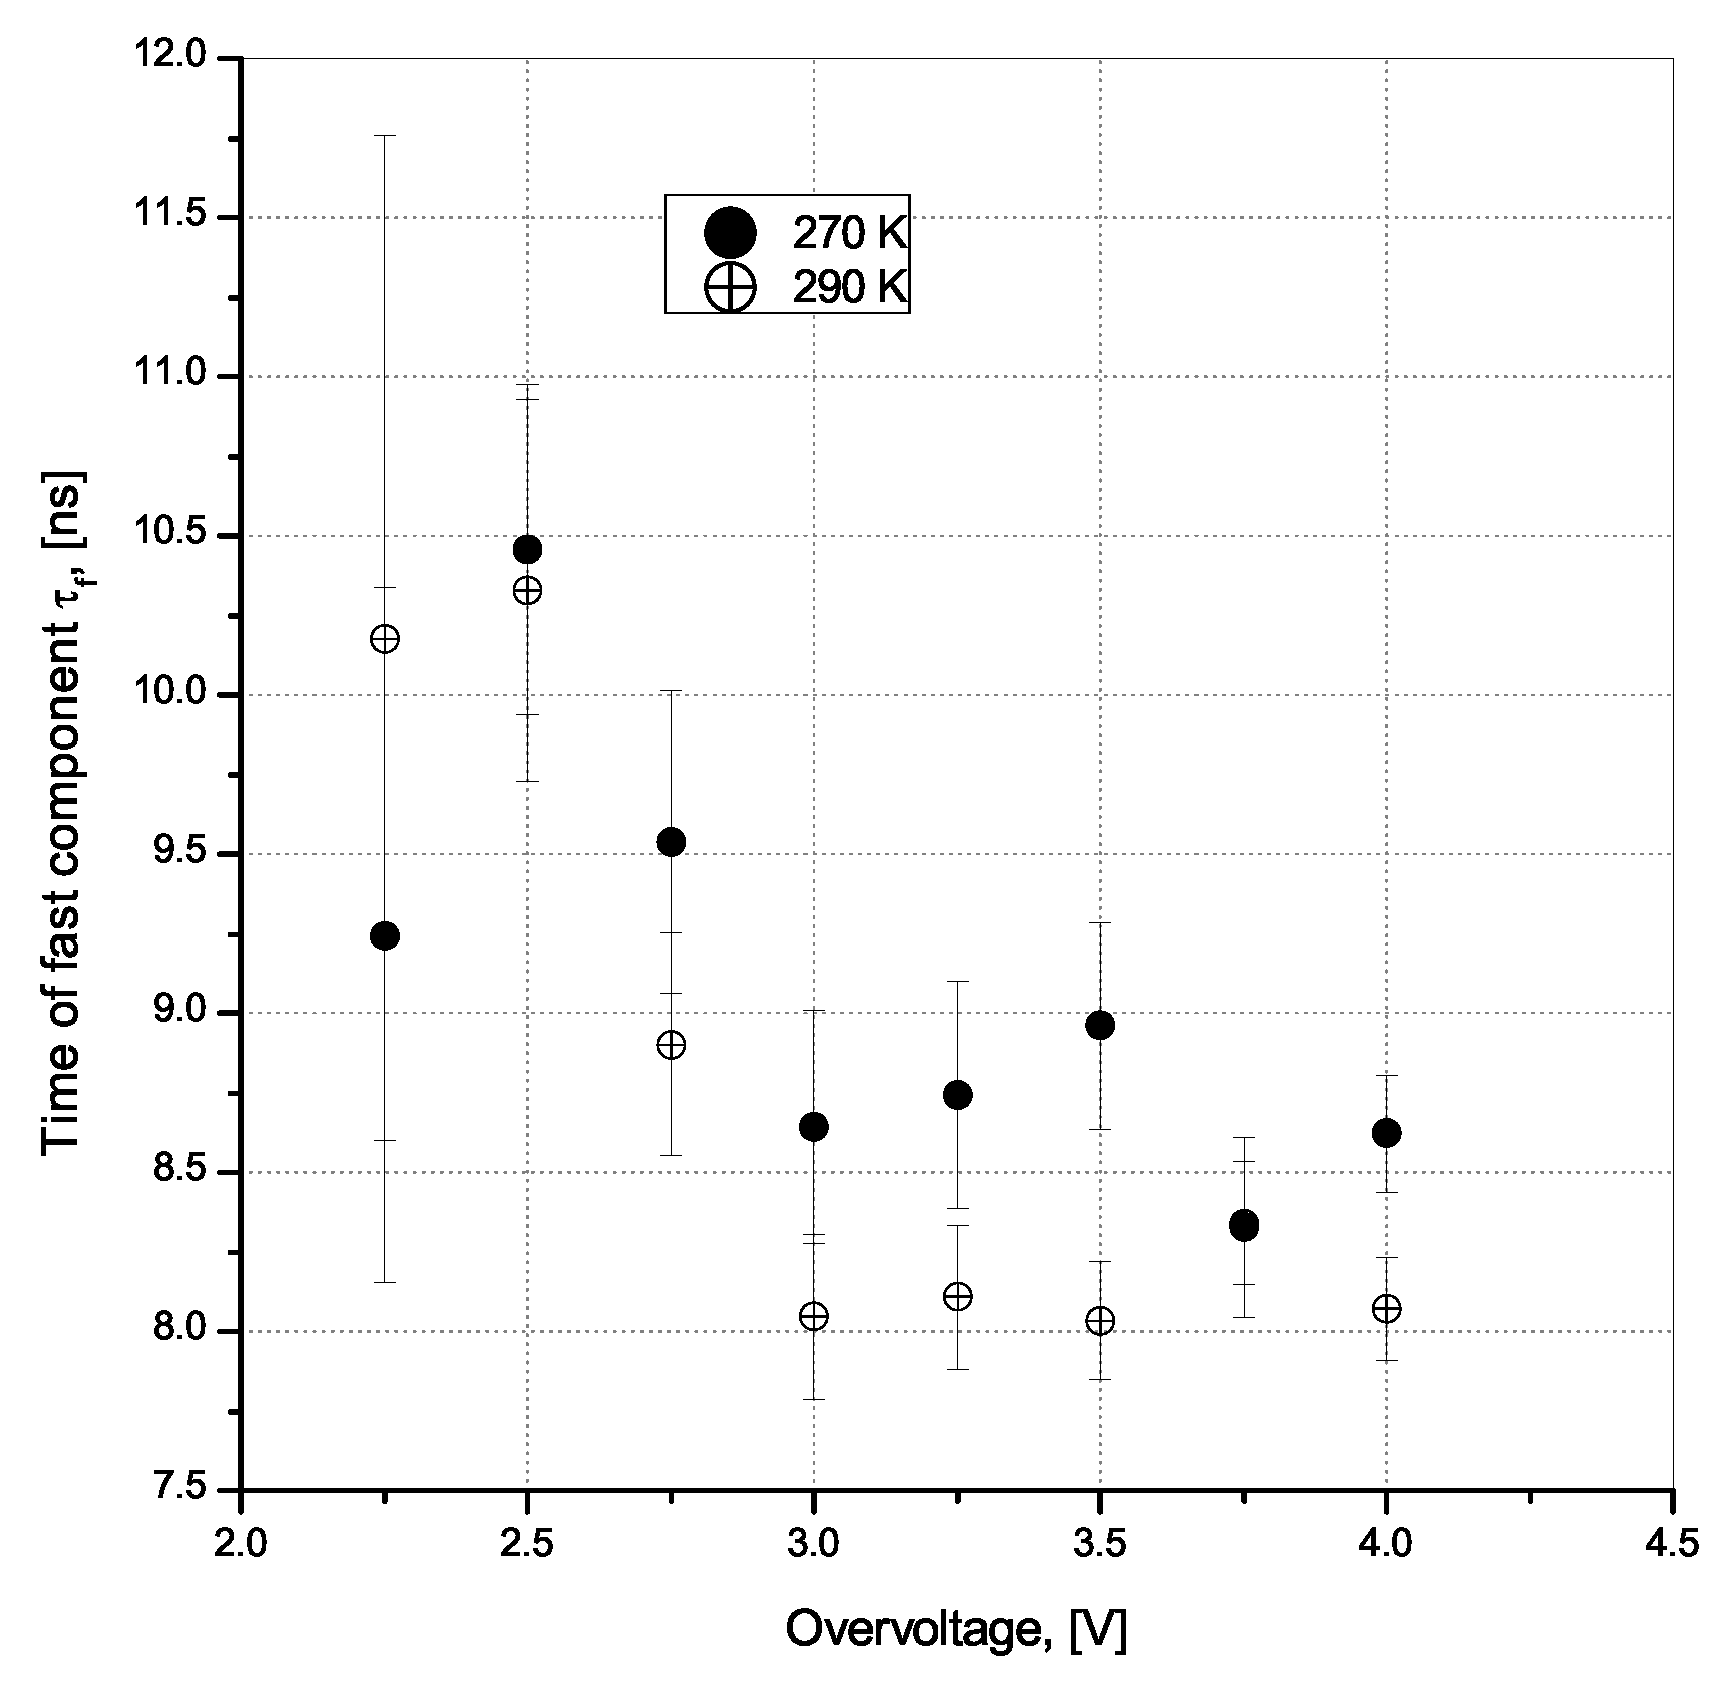
\includegraphics[width=0.47\textwidth]{Hamamatsu_S13360-3050CS_tau_f_vs_V_eng}
\\
\parbox[t]{0.47\textwidth}{\caption{The dependence of the fast component probability $p_{f}$ for after-pulse on the overvoltage at fixed temperature for
Hamamatsu S13360-3050CS. The data were approximated by a quadratic function.}
\label{image:Hamamatsu_S13360-3050CS_p_f_vs_V_rus}}
\hfill
\parbox[t]{0.47\textwidth}{\caption{The dependence of the fast time constant $\tau_{f}$ for after-pulse on the overvoltage at fixed temperature for
Hamamatsu S13360-3050CS.}
\label{image:Hamamatsu_S13360-3050CS_tau_s_vs_V}}
\end{figure}

\begin{figure}[h]
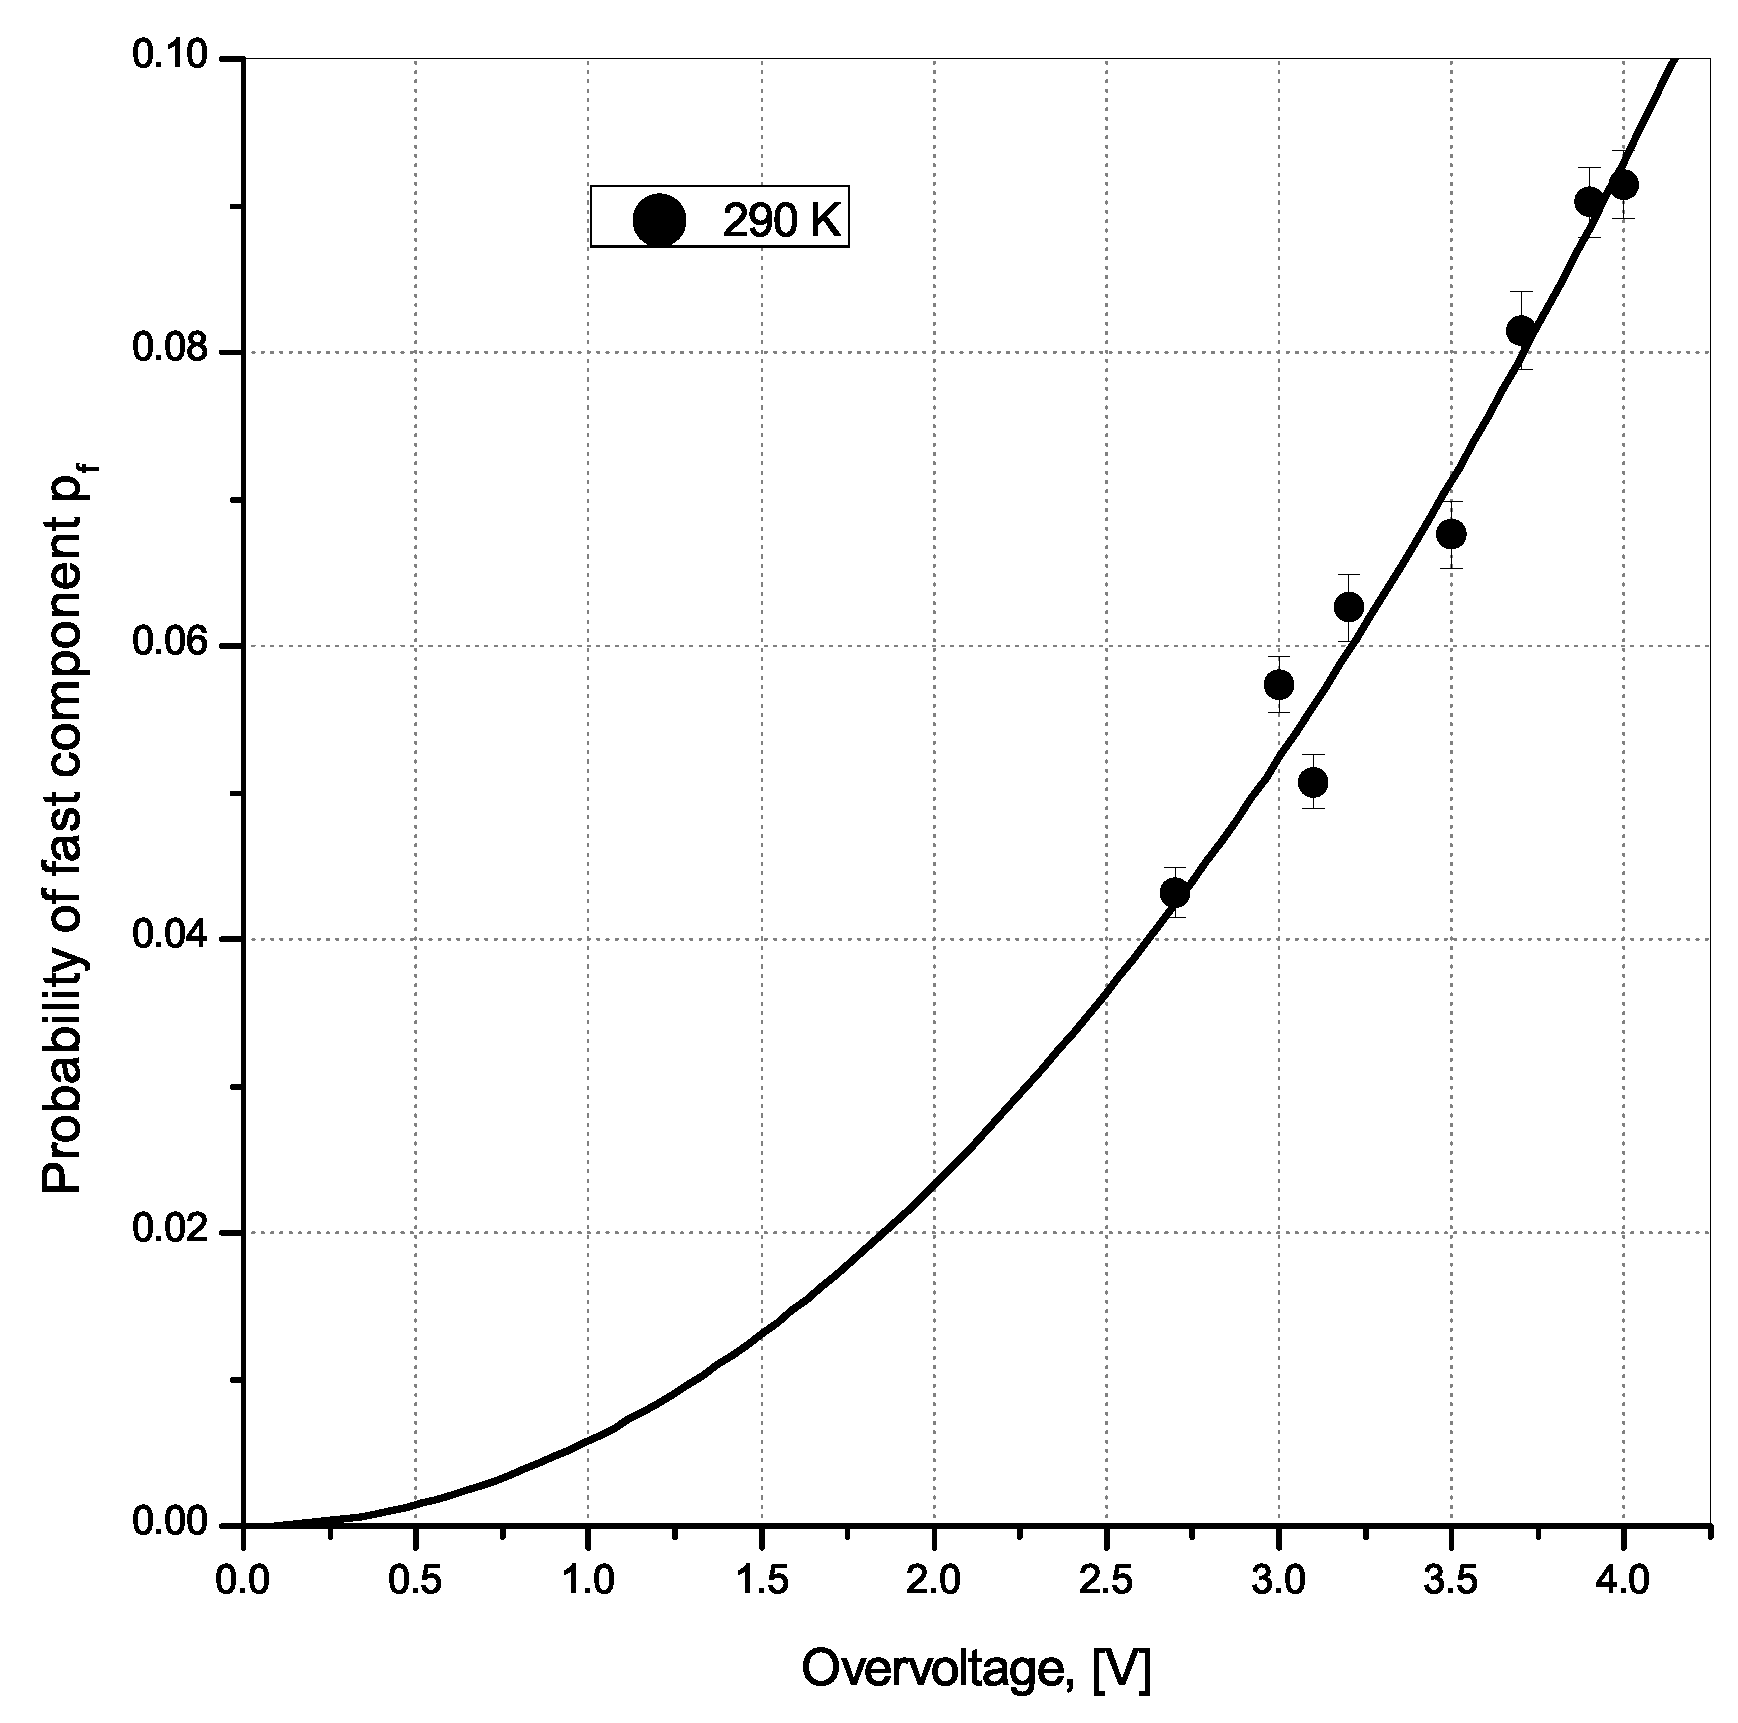
\includegraphics[width=0.47\textwidth]{KETEK_PM1125NS_SB0_p_f_vs_V_eng}
\hfill
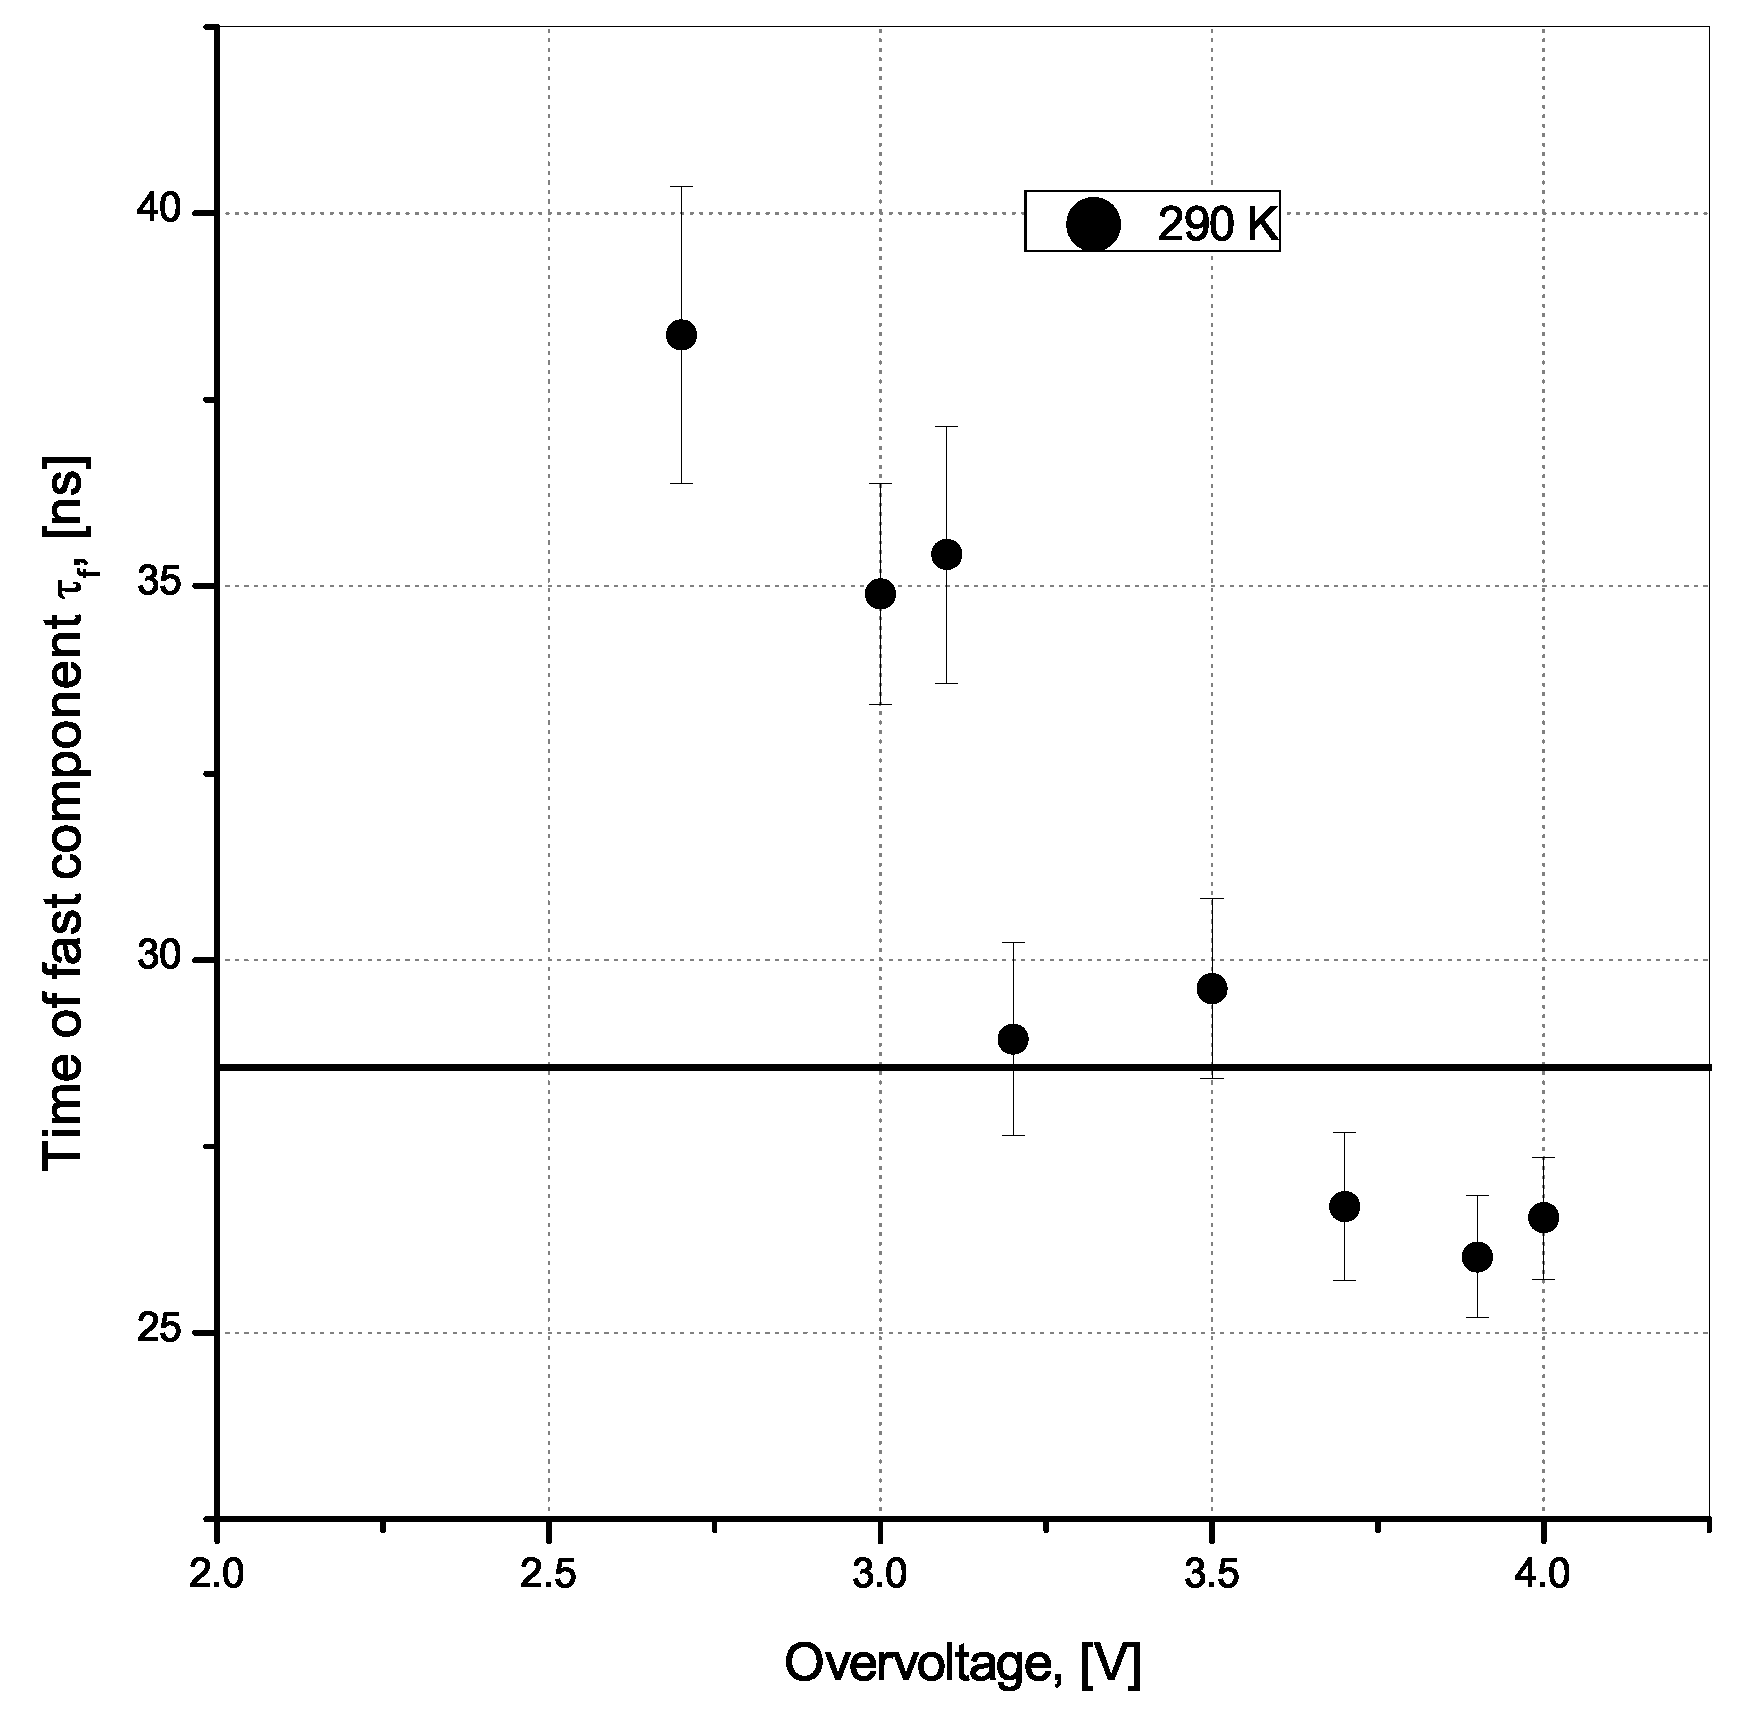
\includegraphics[width=0.47\textwidth]{KETEK_PM1125NS_SB0_tau_f_vs_V_eng}
\\
\parbox[t]{0.47\textwidth}{\caption{The dependence of the fast component probability $p_{f}$ for after-pulse on the overvoltage at fixed temperature for
KETEK PM1125NS-SB0. The data were approximated by a quadratic function.}
\label{image:KETEK_PM1125NS_SB0_p_f_vs_V_rus}}
\hfill
\parbox[t]{0.47\textwidth}{\caption{The dependence of the fast time constant $\tau_{f}$ for after-pulse on the overvoltage at fixed temperature for
KETEK PM1125NS-SB0.}
\label{image:KETEK_PM1125NS_SB0_tau_f_vs_V_rus}}
\end{figure}

The after-pulse probabilities $p_{s}$ and $p_{f}$ at the current accuracy of the measurement are independent of temperature.
At the same time, this probabilities has to have a quadratic dependence on the overvoltage:
\begin{eqnarray}\label{eq:p_f_s_vs_T_V}
p_{i}(\Delta V, T) = k_{i}^{p} \cdot \Delta V^2
\end{eqnarray}

The time constants $\tau_{s}$ and $\tau_{f}$ at a given measurement accuracy are independent on overvoltage.

\section{Conclusions}
In the work were described the algorithms for measurement the breakdown voltage, the dark noise, the probabilities for cross-talk and after-pulsing and after-pulsing time constants for three SiPMs types: KETEK PM1125NS-SB0, Hamamatsu S10362-11-100C and Hamamatsu S13360-3050CS.

Offline signal processing was performed by the pulse approximation with reconstruction of the amplitudes and start time to find these parameters.
Besides the algorithm used, there are three methods.
The first - the measurement of the pulse rate depending on the amplitude threshold.
The second - the integration a signal at a certain time interval and finding a number of events in the peaks.
The third -   signal deconvolution and an approximation the pulse interval spectrum.
The first two methods are rather simple and can be used in online analysis
but they have a serious drawback - after-pulsing probability and after-pulsing time constants can't be be found.
The third method, and the method used in this study require large computing power, however, allow us to find after-pulses parameters.

At achieved measurement accuracy in the temperature range from $0$ to $20 C^{\circ}$ cross-talk probability, after-pulsing probability and after-pulsing time constant are independent on temperature.
SiPMs were checked for compliance with the four neighbors model.
All three types of SiPMs have model discrepancy less than 10\%.

Cross-talk probability for Hamamatsu S10362-11-100C at an operating overvoltage (1 V) is about 12\%, for Hamamatsu S13360-3050CS and KETEK PM1125NS-SB0 (an operating overvoltage is 4 V) is about 6\%. After-pulsing probability for Hamamatsu S10362-11-100C at an operating overvoltage is about 10\% (fast component) � 15\% (slow component).
For Hamamatsu S13360-3050CS and KETEK PM1125NS-SB0 because of the small statistics was studied only the fast component, which is about 10\%.
After-pulsing time constants for Hamamatsu S10362-11-100C are about 35 ns (fast component) and 170 ns (slow component), for Hamamatsu S13360-3050CS - 9 ns, ��� KETEK PM1125NS-SB0 - 28 ns.
Dark noise rate for Hamamatsu S10362-11-100C at an operating overvoltage and $20  \;  ^{\circ}C$ temperature is about $300  \;  kHz / mm^2$, for Hamamatsu S13360-3050CS - $30 \; kHz / mm^2$, for KETEK PM1125NS-SB0 - $80 \; kHz / mm^2$.

Thus, on the basis of the experiments we can conclude that the best candidate for use in counting detectors among the studied SiPMs is Hamamatsu S13360-3050CS which ceteris paribus has a lower dark noise rate and the least after-pulsing time constants.

